\documentclass{article}
\usepackage[utf8]{inputenc}
\usepackage{amsmath}
\usepackage{graphicx}
\usepackage{amsfonts}
\usepackage{algorithm}
%\usepackage{algorithmic}
\usepackage{adjustbox}
\usepackage{listings}
\usepackage{color}
\usepackage{algpseudocode}
\usepackage[backend=biber, style=verbose]{biblatex}
\addbibresource{/home/Documents/PycharmProjects/NEA/references.bib}
\graphicspath{{/home/soham/Desktop/images}}
\definecolor{dkgreen}{rgb}{0,0.6,0}
\definecolor{gray}{rgb}{0.5,0.5,0.5
\definecolor{mauve}{rgb}{0.58,0,0.82}

\lstset{frame=tb,
  language=Python,
  aboveskip=3mm,
  belowskip=3mm,
  showstringspaces=false,
  columns=flexible,
  basicstyle={\small\ttfamily},
  numbers=none,
  numberstyle=\tiny\color{gray},
  keywordstyle=\color{blue},
  commentstyle=\color{dkgreen},
  stringstyle=\color{mauve},
  breaklines=true,
  breakatwhitespace=true,
  tabsize=3
}
\title{Deep Stock Prediction}

\author{Soham Deshpande}
\date{April 2022}

\begin{document}

\maketitle
\subsection*{A Technical Indicator for  liquid asset valuation forecasts using  machine learning techniques }



\clearpage
\tableofcontents

\clearpage

\section {Introduction to the Stock Market}
\subsection{Abstract}
\normalsize{In recent years the fast-growing financial markets opened new horizons for\\ investors and at the same time brought new challenges for financial analysts in their efforts to make effective decisions and reduce investment risks.
The stock market is a highly dynamic and complex system where factors affecting the price are not limited to the economic world, rather in recent years the political climate and social media playing a bigger role. This has resulted in a highly stochastic, chaotic market. As with the other industries, the amount of data being created every day can be overwhelming and often hard to understand and decipher for someone with limited experience. This problem can be seen as one for computer science and mathematics.
In the past decades, effective prediction models, both linear and machine learning tools have been explored. In recent years the research into deep learning has rapidly accelerated the progress made in prediction software. The motivation behind this paper is to describe and show an implementation of a deep learning model to help predict the price of stocks.
\\
Keywords:
Stock market prediction, deep learning, transformers, attention, feedforward neural network, temporal fusion transformers
}

\section{Introduction}
The model I will be exploring is a transformer-based deep learning architecture that takes advantage of attention, more specifically multi-head attention in my implementation.
Many models use ARIMA(Auto-Regressive Integrated Moving Average) but I am proposing using transformers with multi-head attention, something that I will talk about later on, to help the model ‘learn’ about the stock rather than just trying to fit a curve on it based on the last few data points. The benefits of learning allow the model to consider previous experience instead of just looking at a few, previous data points. This technique will hopefully result in a higher accuracy compared to ARIMA. Other implementations have managed an accuracy of 94\%(Zolkepli and Divino, n.d.) so I will be aiming to stay within 5\%. The reduced target comes down to a few factors such as limited access hardware, not enough time to optimise my program for the hardware as well as a few other factors.
\clearpage
\section{Client Requirements}

Q\&A
\\\\
What factors would you consider essential to be considered when evaluating the performance of a stock?\\
When I buy a stock I firstly look at what sector the company makes most of its profit from, taking BP as an example, I would look at how stocks in the oil industry are performing. This includes ETFs such as Brent Oil(BNO) or Wisdom Tree. After that, I would normally look at the previous performance of the stock I am interested in. This includes patterns in dips and highs at times such as Christmas. I would also look at the previous month to give a general indication. The next thing I consider is the volume traded. This shows the popularity of the stock. After that, I often search for any news articles related to the stock or the sector. Here I am looking for any expected announcements such as the incoming of a new CEO, an increase in dividends or new projects.
\\\\
What would help build your confidence in the system?
\\
I would like a probability associated with all the predicted prices, similar to a confidence level. This would allow me to make an independent decision on whether the prediction is likely or not. Similarly, I would like the software to alert when a change in a price is expected given that the confidence level is high. Personally, confidence level presented as a percentage is what I would like.
\\\\
What would help the software be more “intelligent” and useful?\\
Along with the prediction and confidence level, I would like the system to make a suggestion on whether I should buy, short or sell the stock. An explanation for this decision is not necessary. The program should also be able to track all of the items in my portfolio and, again, give alerts specific to the stocks I am currently holding.
\\\\
How far into the future do you want the predictions to be?\\
I think there’s a balance to be found. A prediction should not be just for a day as this requires me to have the same commitment as a day trader. At the same time, a prediction should not be too far into the future like in 6 months time. For my trading style, a prediction of 1 week to 3 months gives me a good indication of what to expect. A day trader might want a prediction of 1 hour to 1 week so I think having the option to choose how far into the future I want the predictions to be is a feature I would really appreciate.
\\\\
Questions from the client:\\
\\
Will you be handling real-time data?\\
This is a feature I will consider near the end of my project due to the complexities involved. This will help my program to be more useful in the real world but is very hard to do with the limited resources I have access to.



\section{Analysis}
\subsection{Stock prediction techniques}
Stock prediction is a problem that requires time series analysis. Time series analysis is the technique of analysing sequential data.
In the current market, a couple of techniques are used to analyse and predict the price. In this section, I will discuss a few multivariate time series models.

\subsection{ARIMA}
Autoregressive integrated moving average is a common method used to perform time series analysis.
(Hyndman and Athanasopoulos, 2018)
In a regression model, we forecast the variable of interest using a linear combination of predictors. Autoregression focuses on using a linear combination of past values and the variable itself to predict the variable of interest. The term autoregression indicates that it is a regression of the variable against itself.

\begin{equation}
    y_t = c + \phi_1 y_{t-1} + \phi_2 {t-2} + ... + \phi_p y_{t-p} + \epsilon_t
\end{equation}

These models are very good at handling different time series patterns. Changing the parameters, $\phi$ result in different patterns. $\epsilon$ is the error term; changing this will change the scale of the series. This model is very effective when it comes to stock prediction and so will therefore provide a baseline when it comes to the accuracy of the model.
\begin{figure}[h]
    \centering
    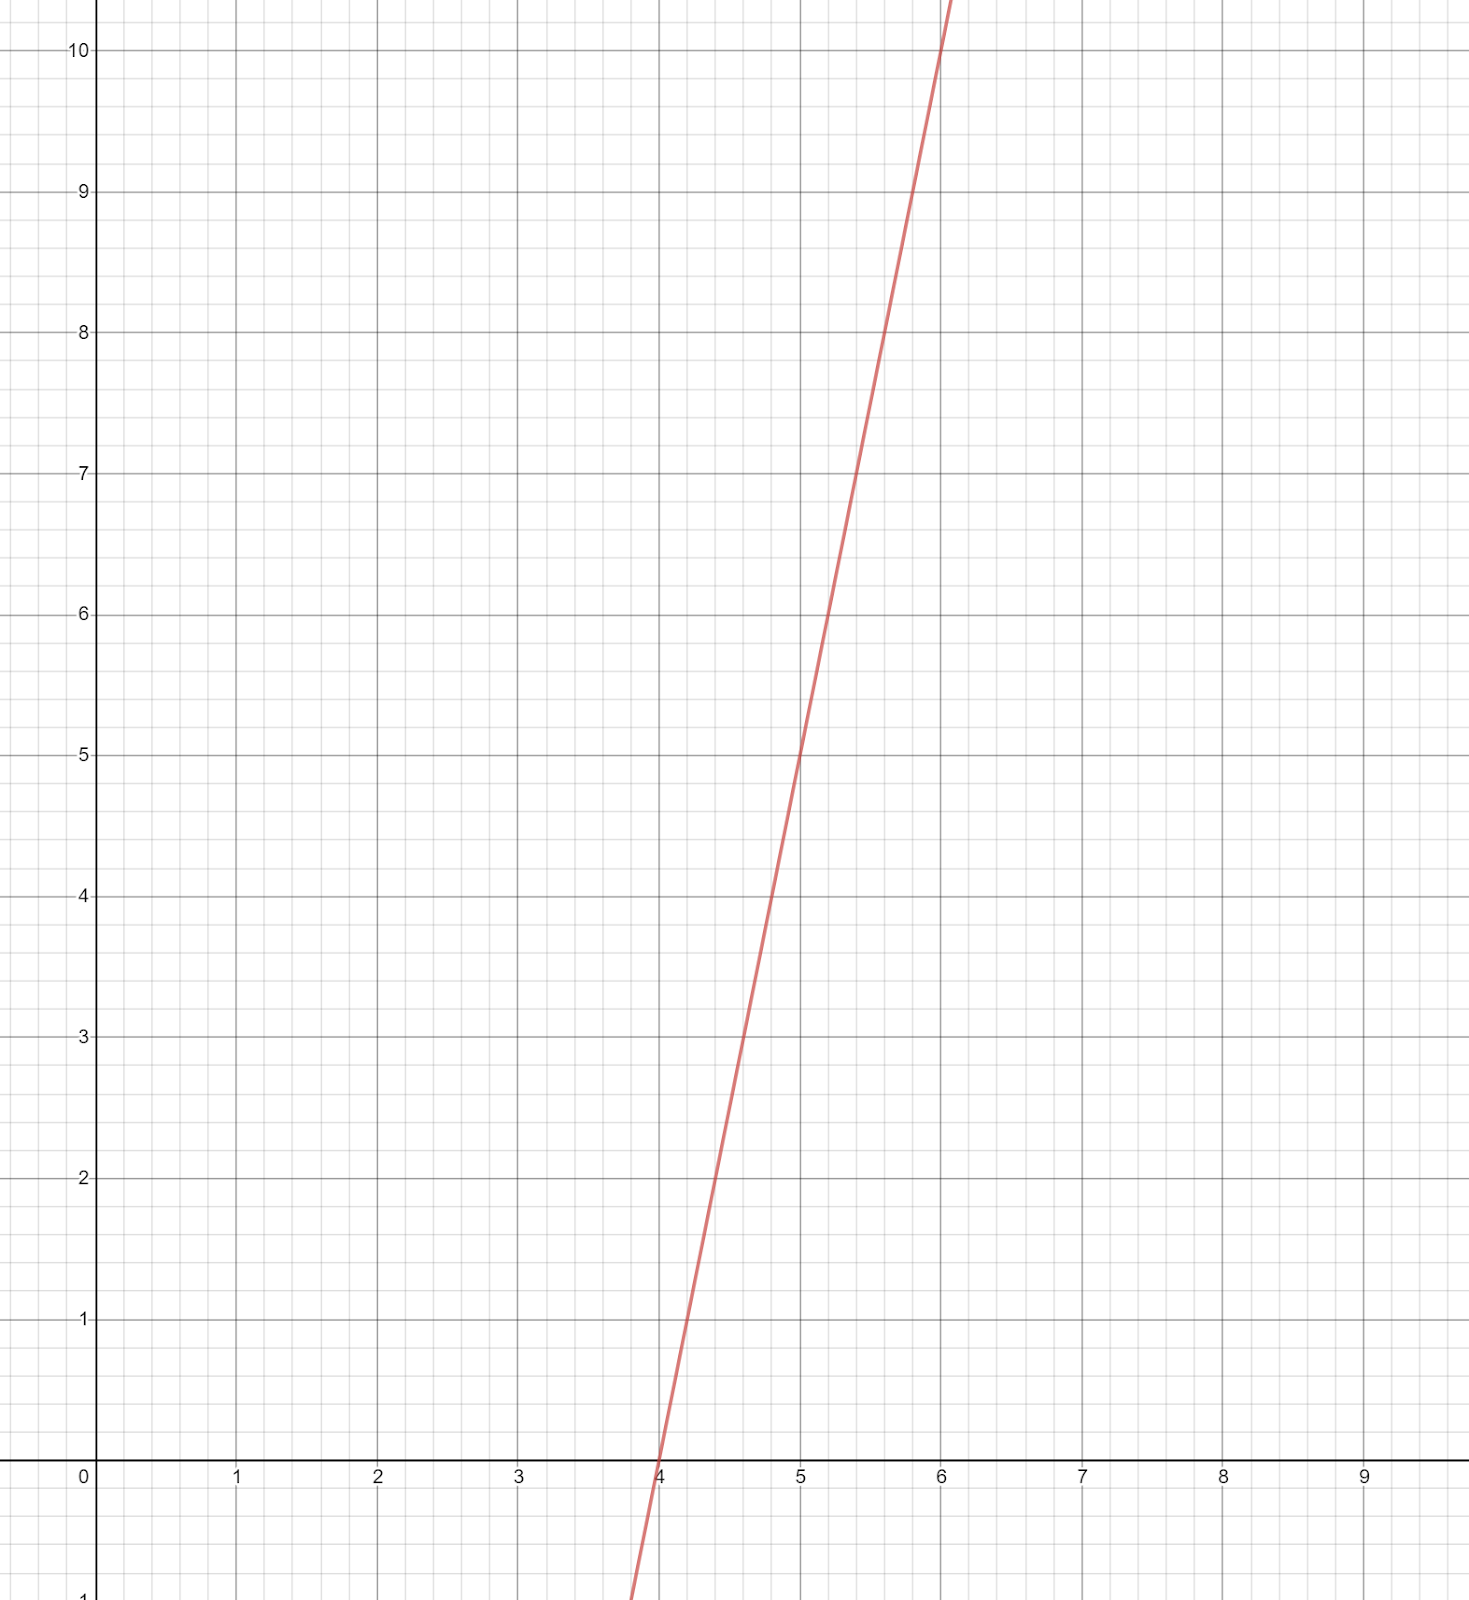
\includegraphics[scale=0.1]{arima1}
    \caption{Plotting the data }
\end{figure}
The image above shows an implementation of auto regression on FTSE 100 data from 2010 to 2020. Green dots represent the predicted values while the red dots represent the actual values.
\clearpage
\begin{figure}[h]
    \centering
    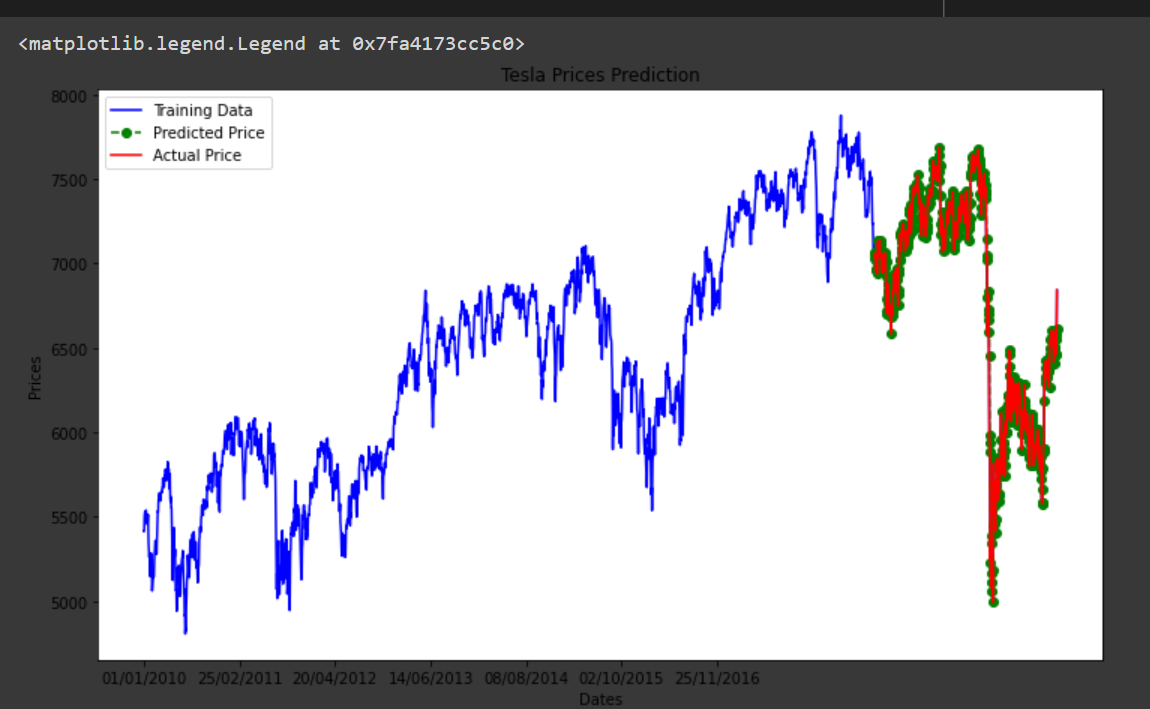
\includegraphics[scale=0.21]{arima2}
    \caption{Using ARIMA on test data }
\end{figure}
Figure 3 shows the accuracy of the model at a respectable 89.21\% when using MSE as the loss function.
\begin{figure}[h]
    \centering
    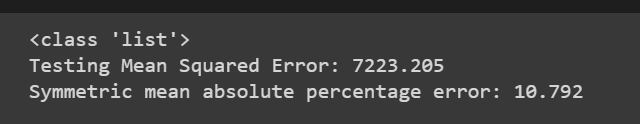
\includegraphics[scale=0.35]{arima3}
    \caption{MSE Loss using ARIMA }
\end{figure}

\subsection{Neural Networks}
The research done in the 1990s have helped set up the foundations for a mathematical model that is today known as machine learning. This mathematical process aims to replicate the brain through the use of several functions and calculus. This replication comes in the form of neurons in a neural network. In the following paragraphs I will proceed to explain a type of neural network known as a ‘Convoluted neural network’ before proceeding to describe an evolution, the ‘Recurrent neural network’.


\subsection{CNN}
The neural network is heavily dependent on the maths surrounding gradients, in particular differentiation. The main components of a neural network include: an activation function, layers, a loss function and an optimiser.
\\
Similar to the human brain, a neural network is made up of many neurons. These neurons are information processing units that are fundamental to the operation of a neural network. The structure of a neuron is shown in figure 11 but is represented by a subscript k.  A basic neural network consists of 3 main parts: a set of connecting links between neurons, an adder and an activation function.
\\
The set of links each have a weight assigned to them. They work by taking input signals, often as vectors, and then multiply these by the weights they are assigned. This process is shown in figure 11. After that each vector is added together before a fixed bias is applied. To simulate the process of a neuron turning on and off, an activation function is used. These are mathematical functions and are described in the following paragraphs.

\subsection{Activation Functions}
To summarise the behaviour of an activation function, it can be compared to a transistor; it only activates at a certain threshold.  These try to replicate how the neurons behave in our brain.
The most common activation functions are shown below along with their equation.

\begin{itemize}
    \item Binary step function
    \begin{itemize}
        \item \begin{align*}
            u(x) = 	1 \mbox{ if }  x \geq 0 \mbox{ or } 0 \mbox{ if } x <  0
        \end{align*}


     \begin{align*}
            Y = u(x-3)
        \end{align*}
        \begin{figure}[h!]
            \centering
            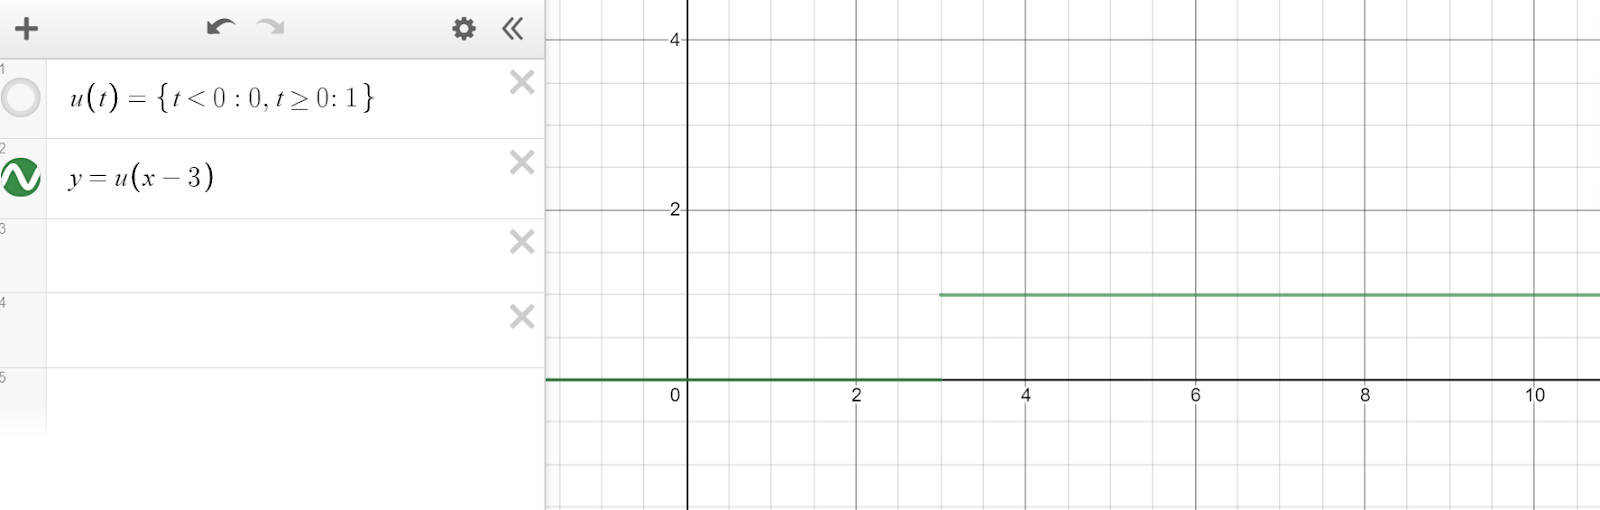
\includegraphics[scale=0.15]{binarystep}
            \caption{Binary step function}
        \end{figure}
    \end{itemize}


    \item Linear Function
        \begin{itemize}
            \item \begin{equation*}
            f(x) = mx
        \end{equation*}
        \end{itemize}

\clearpage
    \item Sigmoid
        \begin{itemize}
            \item
        %Values range from 0 to 1\\
        %\begin{align*}
            $$\sigma(x)  =\:\frac{1}{\:1+e^{-x}}$$
            $$\frac{d}{dx} =$$
            $$f  = 1 \quad f' = 0$$
            $$g  = 1 + e^{-x} \quad g' = -e^{-x}$$
            Using the quotient rule:
            $$= \frac{e^{-x}}{{(1+e^{-x})}^2}$$
        %\end{align*}
            This can also be written as:
            $$\sigma'(x) = \sigma(x)(1-\sigma(x))$$

        \end{itemize}


    \item Tanh
        \begin{itemize}
        \item $tanh(x) = 2\sigma(2x)-1$
        \item Values range from -1 to 1
        \end{itemize}
        \begin{figure}[h!]
            \centering
            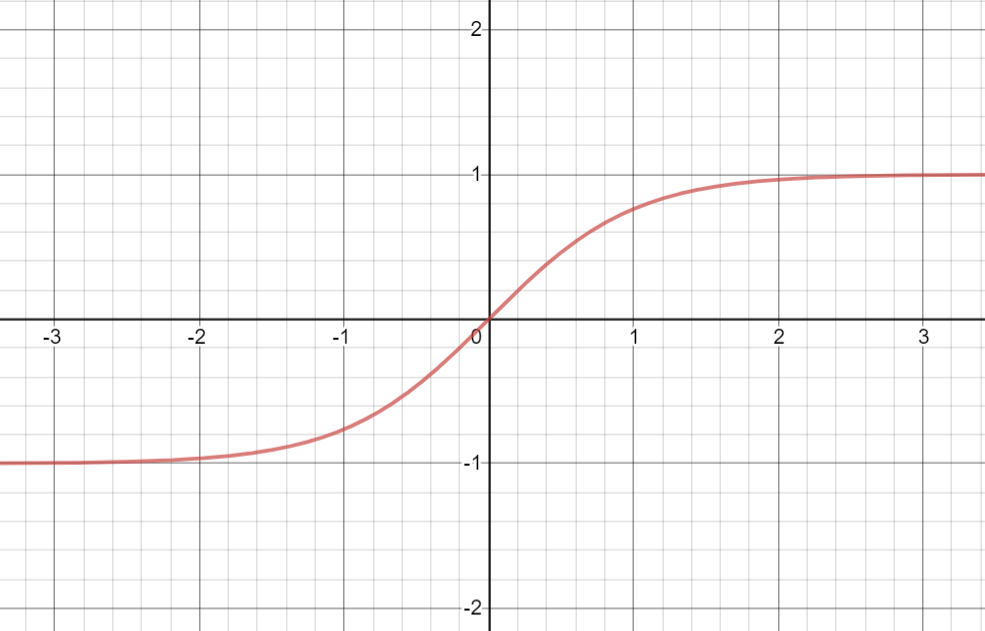
\includegraphics[scale=0.15]{tanh}
            \caption{Tanh function}
        \end{figure}


    \item ReLU(Rectified Linear Unit)
        \begin{itemize}
            \item Neurons will only deactivate if the output of the linear transformations less that 0\\
            Also a leaky version of ReLU present
        \end{itemize}
        \begin{figure}[H]
            \centering
            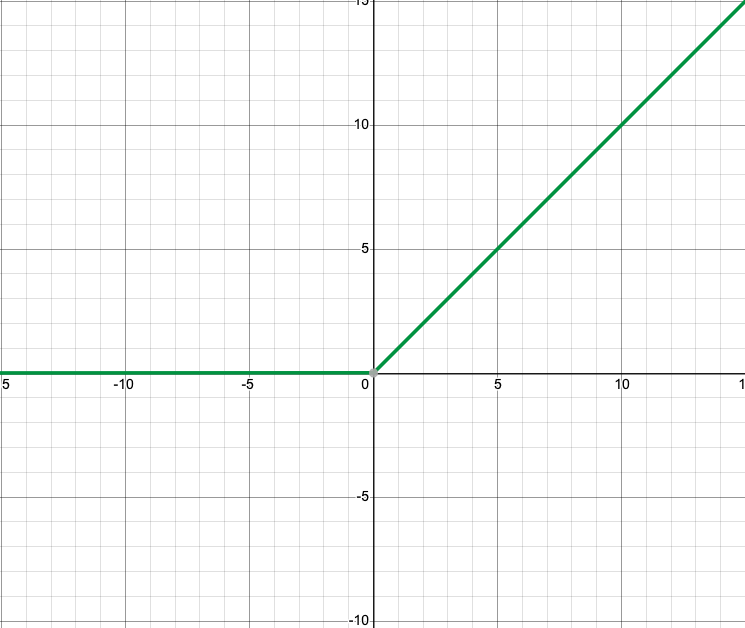
\includegraphics[scale=0.15]{relu}
            \caption{ReLU function}
        \end{figure}

    \item Softmax
        \begin{itemize}
            \item Returns the probability for a data point belonging to each individual class
            $$\sigma(\hat{z})_i = \frac{e^{zi}}{\sum_{j=1}^{k}e^{z_j}}$$
            Below is a description of the softmax function: (Versloot, 2020)\\

This can be described as the following: for each value in our input vector, the Softmax value is the exponent of the individual input divided by a sum of the exponents of all the inputs.
\\
This ensures that multiple things happen:
\\
Negative inputs will be converted into nonnegative values, thanks to the exponential function.\\
Each input will be in the interval (0,1)
As the denominator in each Softmax computation is the same, the values become proportional to each other, which makes sure that together they sum to 1.\\
\\
These properties allow us to interpret them as probabilities.
\\
To make sure these values are actually valid probabilities, it can be checked against Kolomogorov’s probability axioms.
\begin{itemize}
    \item Each probability must be a nonzero real number. This is true for our outcomes: each is real-valued, and nonzero.
    \item The sum of probabilities must be 1. This is also true for our outcomes: the sum of cut off values is$\approx$ 1, due to the nature of real-valued numbers. The true sum is 1.
\end{itemize}
Here is an example of the function
\begin{figure}[H]
            \centering
            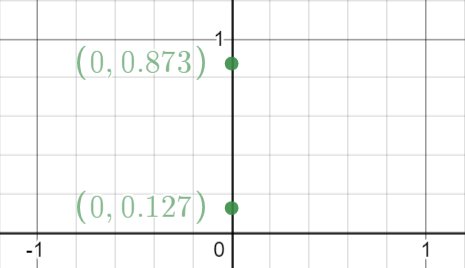
\includegraphics[scale=0.25]{softmax}
            \caption{Where a = 6.638 and b = 4.71}
        \end{figure}
        \end{itemize}
        In the equation above, $\hat{z}$ is the input vector to the softmax function, made up of ($z_0, ... z_k$)\\
        $z_i$ are All the $Z_i$ values are the elements of the input vector to the softmax function, and they can take any real value, positive, zero or negative. For example a neural network could have output a vector such as (-0.62, 8.12, 2.53), which is not a valid probability distribution, hence why the softmax would be necessary.\\
        $e^{z_ii}$ is the  standard exponential function is applied to each element of the input vector. This gives a positive value above 0, which will be very small if the input was negative, and very large if the input was large. However, it is still not fixed in the range (0, 1) which is what is required of a probability.\\
$\sum_{j=1}^{k}{e^{z_j}}$ is the term on the bottom of the formula is the normalization term. It ensures that all the output values of the function will sum to 1 and each be in the range (0, 1), thus constituting a valid probability distribution.\\
        $k$ is the number of classes in the multi-class classifier.
\end{itemize}
\begin{itemize}
\item ELU(Exponential linear unit)\\

\end{itemize}
The exponential linear unit was designed to fix some of the problems with ReLUs. This function has a parameter that is picked; a common value is between 0.1 and 0.3.
\begin{equation*}
            ELU(x) = 	x \mbox{ if }  x > 0 \mbox{ or } \alpha(e^{x}-1)  \mbox{ if } x <  0
        \end{equation*}
This  equation tells us that if the input, x, is greater than 0 then the output is the same as a RELU, y=x. If the input drops below 0, the value becomes slightly smaller than 0. This value will be modelled using (ex-1)where we choose a value for . The exponential operation makes this function more computationally expensive than a vanilla ReLU. The exponential function helps fix the vanishing gradient problem often associated with ReLUs. An advantage is that the ELU produces negative values which allows them to push mean unit activation close to zero, a bit like batch normalisation but with lower computational complexity. Mean shifts towards zero help speed up learning.
\begin{figure}[H]
            \centering
            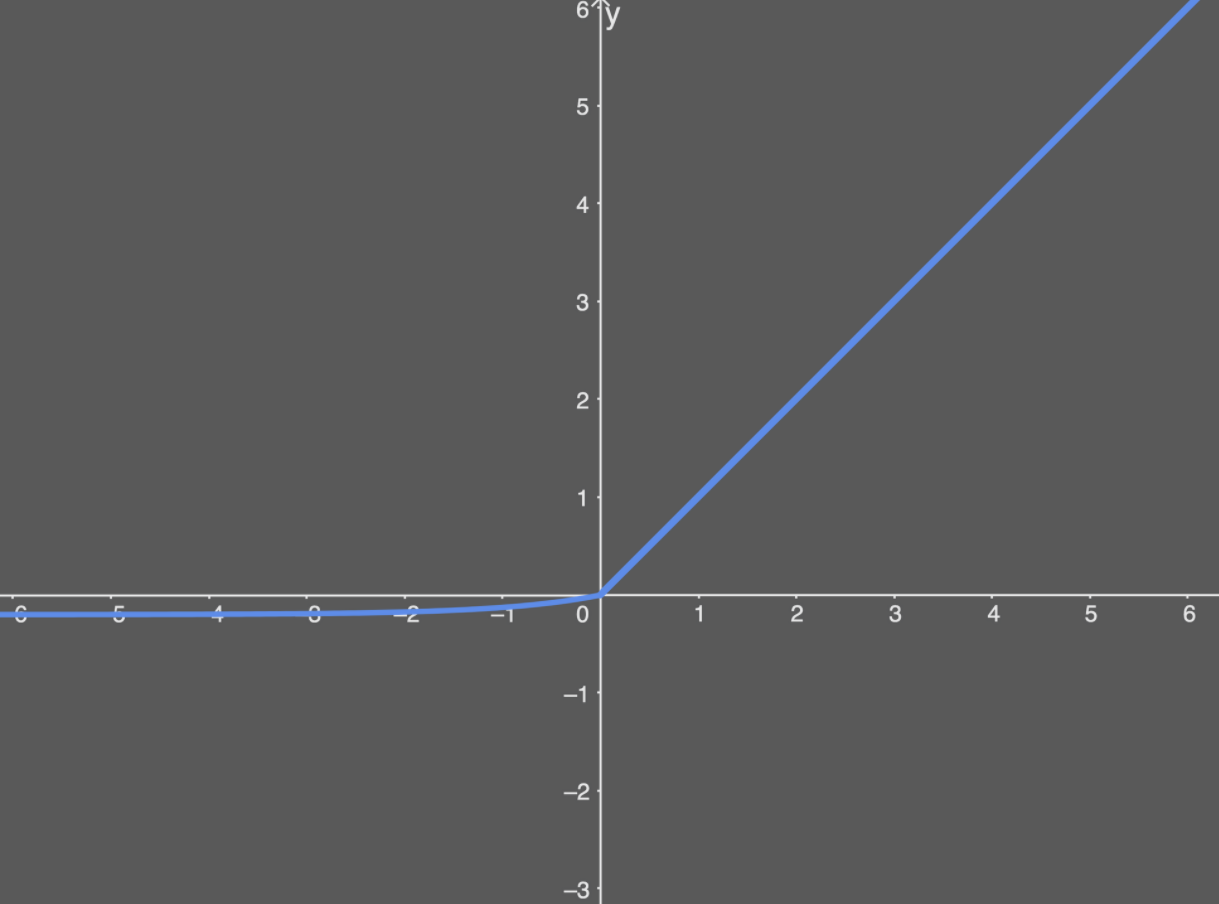
\includegraphics[scale=0.15]{elu1}
            \caption{ELU function}
        \end{figure}
The derivative can be written as\\
\begin{equation*}
            ELU'(x) = 	1 \mbox{ if }  x > 0 \mbox{ or } \alpha(e^{x})  \mbox{ if } x <  0
       \end{equation*}
The exponential function helps make this function differentiable at all points.  Below is the graph for the derivative:
\begin{figure}[H]
            \centering
            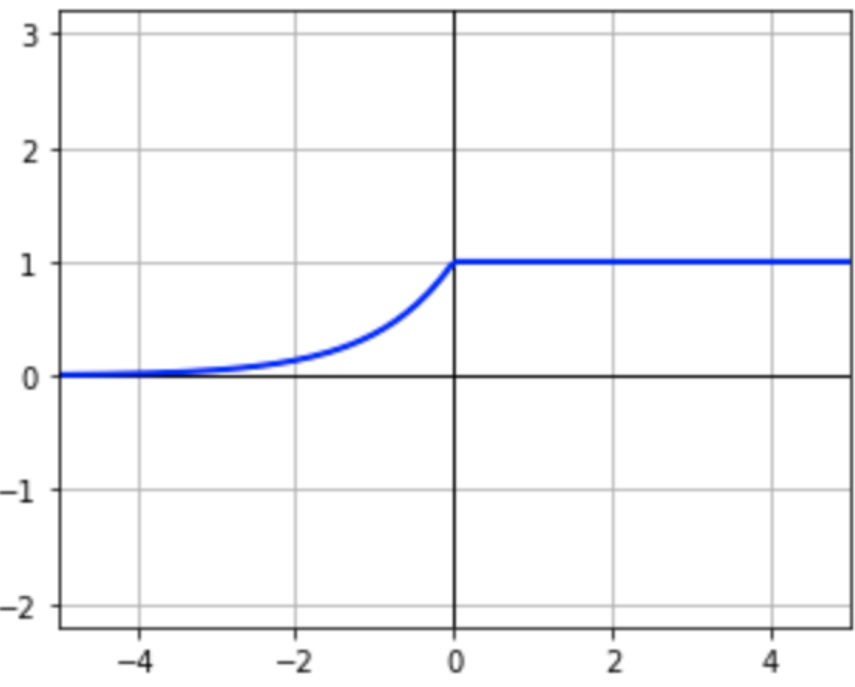
\includegraphics[scale=0.15]{eluderiv}
            \caption{ELU derivative function}
        \end{figure}

\end{itemize}

\subsection{Layers}

As shown in the figure below, in between the input and output layers there are hidden layers.  These layers contain many neurons. The equation that is used to model these neurons is shown in the second image, I have used the sigmoid function as an example of the calculation that may happen at a neuron. The summation of the weights multiplied by the input activity. A bias is then applied before the activation function, a sigmoid in my example, is applied to the result to determine whether the neuron should turn on or not.
\begin{figure*}[h!]
            \centering
            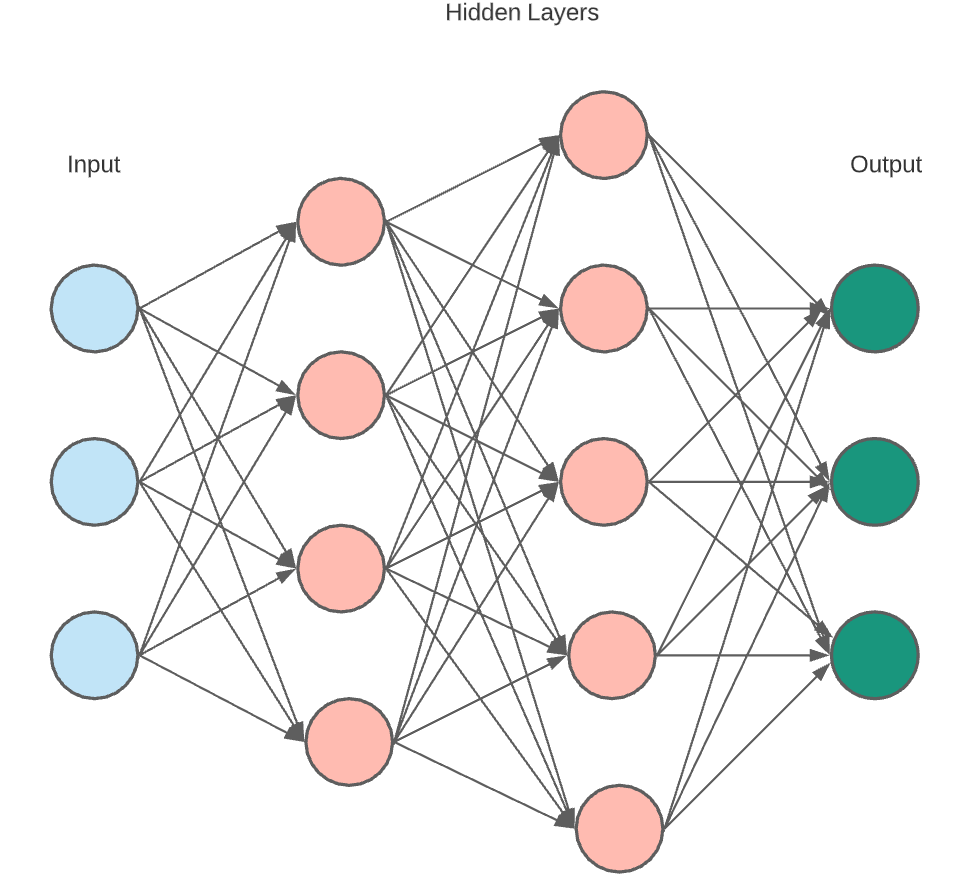
\includegraphics[scale=0.15]{layers1}
            \caption{Layers shown in a neural network}
        \end{figure*}
\begin{figure}[h!]
            \centering
            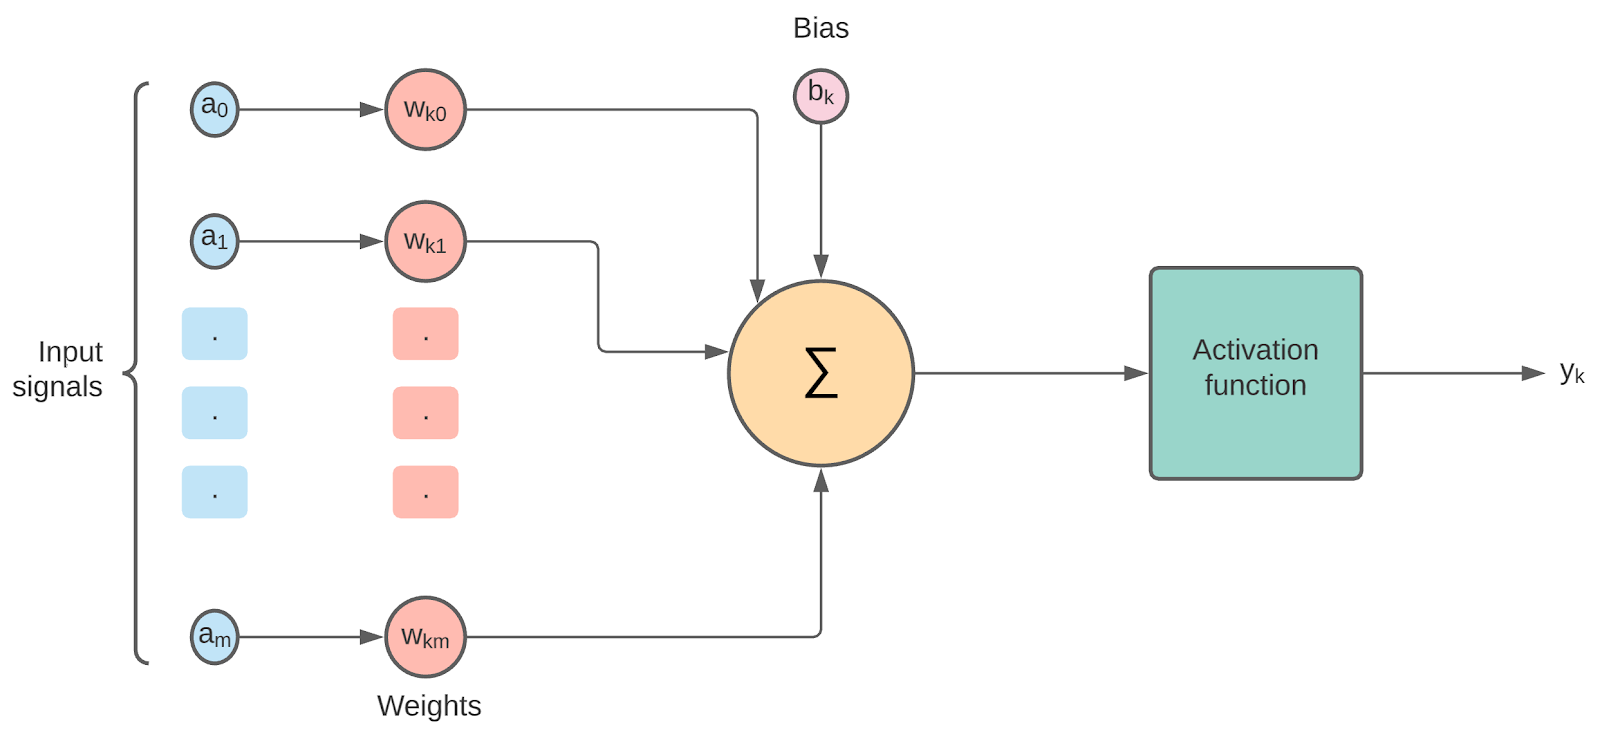
\includegraphics[scale=0.15]{layers2}
            \caption{Neuron represented mathematically}
        \end{figure}

\subsection{Neurons and Equations}
The neurons can be modelled using the equations given below in the equation $$a = \sigma(w \times a + b)$$
Here $a$ is the activity, the activity of the neuron, $\sigma$ is the activation function, $w$ is the weight and $b$ is the bias.
The equation shows that the activity is modelled by multiplying the previous activity by a weight that is changed during the whole learning process, before a constant bias is applied. The equation below shows a more general equation where the letter L represents a neuron in current time and so L-1 is the activity of the previous neuron.
$$a^{L} = \sigma(w^{L}\times a^{L-1} + b^{L})$$
Another way to write this is:\\
$$\sigma((\sum_{j=0}^{n}w_j\cdot a_j)+b)$$

\subsection{Loss Functions}

A loss function is what ultimately gives the neural network its intelligence. At its core it’s a method evaluating how well the algorithm models the data. If the predictions are off by a high margin then a high loss will be calculated. If the margin of error is lower, a lower number will be calculated showing that your predictions are quite close. This loss is also commonly referred to as the accuracy. The goal is to get your loss as low as possible or can be referred to as achieving a high accuracy.  There are many functions that can be used to determine the loss but the most common are root mean squared error, absolute error loss and binary cross entropy loss. Lots of neural networks have custom loss functions that are dependent on the purpose they are serving. A very strict loss function that amplifies the loss is more typical in places where the loss must be kept at a minimum such as stock prediction.

\subsection{Feed Forward and Back propagation}
For the neural network to truly learn, it must go through a process called back propagation. This is an algorithm that is used in supervised learning and uses a concept called gradient descent.
One way to think about a loss function is to imagine it being a black box that works out an equation, say y =  to get you from the domain to the range. Now this equation can be plotted, figure 2 and we can see that there are a few things to observe about this graph. Calculus tells us that the turning points happen when the gradient of a curve, that can be worked out using differentiation, is 0. The second step is to work out the second derivative and that will  tell us whether the point is a maxima or minima. Where $\frac{d^{2}y}{dx^{2}} > 0$, the point can be described as a minimum and when $\frac{d^{2}y}{dx^{2}} < 0$, the point can be described as a maximum. The minimum point that occurs when $\frac{dy}{dx}$ (the gradient)is 0, on the graph below it happens at the point (3,0).

\begin{figure}[H]
            \centering
            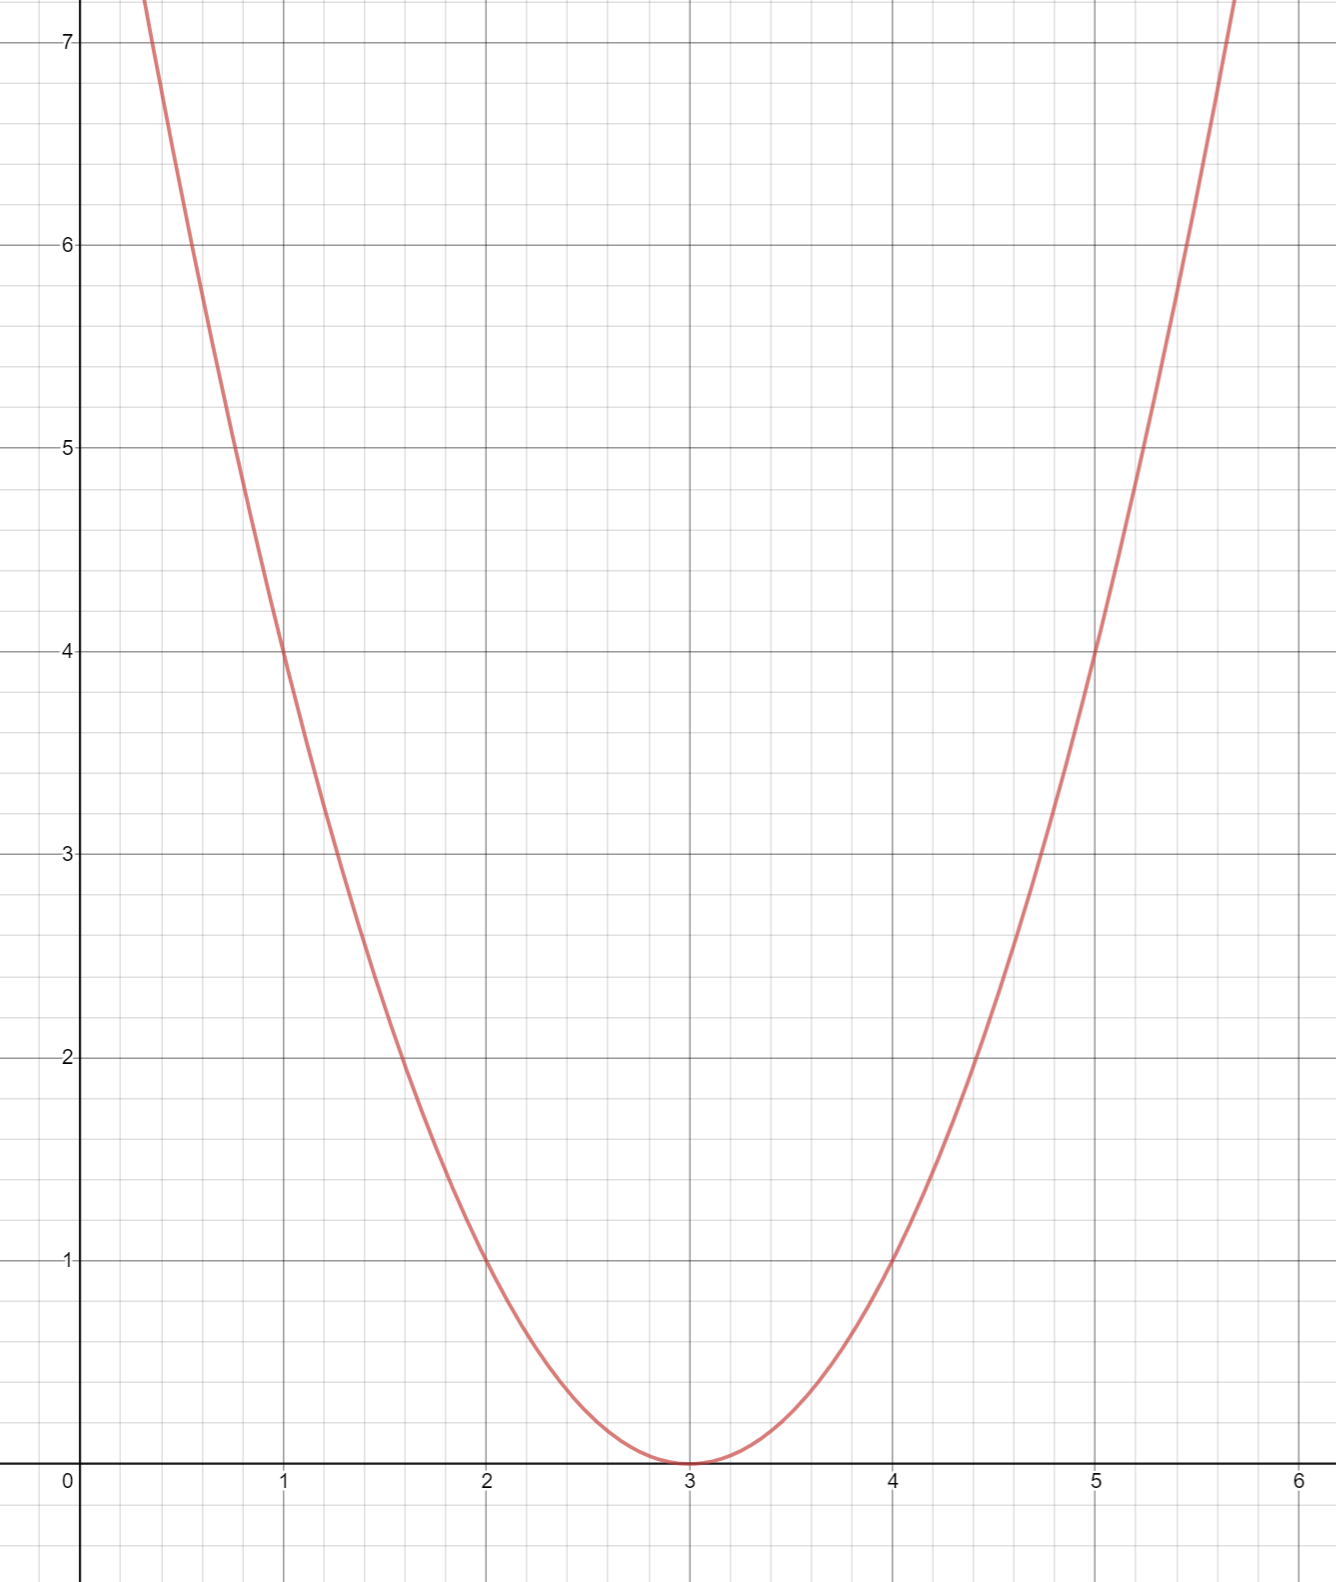
\includegraphics[scale=0.15]{ff1}
            \caption{}
        \end{figure}
Consider $w$ to be one of the weights discussed in the previous section.\\
If $w<3$, we have a positive loss function, but the derivative is negative, meaning that an increase of weight will decrease the loss function.\\
At $w=3$, the loss is 0 and the derivative is 0, we reached a perfect model, nothing is needed.\\
If $w>3$, the loss becomes positive again, but the derivative is as well positive, meaning that any more increase in the weight, will increase the losses even more.\\
To try and decrease this loss, at $w<3$ you should increase the weight and at $w>3$ you should decrease the weight.\\
\\
The equation for working out the new weight is shown below where $w_n$ is the weight, $C$ is the cost function and $\alpha$ is the learning rate(which is a constant). \\

$$new\hspace{3}w_n = (old\hspace{3} w_n) - \alpha \cdot \frac{\partial C}{\partial w_n}$$
%error above, not too sure why

\subsection{Backpropagation}
The goal of backpropagation is to minimise the error function by changing the weights of the individual neurons. The formulation of the complete backpropagation algorithm can be proven by induction to show that it works with differentiable activation functions at its nodes.
\\
For this proof, the assumption has been made that the neural network is one with a single input and single output. To simplify the proof, instead of carrying a bias term, let us assume that each layer $V^{(t)}$ contains a single neuron $v_o^{(t)}$ that always outputs a constant 1 thus the output of a neuron is given by $$\sigma(\sum w_{i,j}v_j^{t-1})$$ We next wish to compute the derivative $\nabla f_w$. Now suppose neuron $v_i^{t}$ computes:
$$v_i^t(x) = \sigma(u_i^t(x))$$
Then using the chain rule we can obtain that\\
$$\frac{\partial f}{\partial w_{i,j}} = \frac{\partial f}{\partial u_i^t}\cdot \frac{\partial u_i^t}{\partial f} = \frac{\partial f}{\partial u_i^t}v_i^{(t-1)}(x)$$\\

Thus to compute the partial derivative of a single weight, it is enough to compute $\frac{\partial f}{\partial u_i^t}$.
We can now focus on computing $\frac{f}{\partial u_i^t}$. Now suppose f is a function of $u_1^t, \cdots, u_m^t$, which we are in turn function of some variable $z$ then we have by chain rule:
$$\frac{\partial f}{\partial z} = \sum_{i=1}^{m}\frac{f}{\partial u_i^t}\cdot \frac{\partial u_i^t}{\partial z}$$
Now if $z = u_n^{t-1}$ is the output of some neuron in a previous layer: The calculation of $\frac{u_i^t}{\partial u_n^{t-1}}$ is easy for our choice of activation function
$$u_i^t = \sum w_{i,j}\sigma(u_j^{t-1}) \rightarrow \frac{u_i^t}{u_n^{t-1}} = w_{i,n}\sigma'(u_n^(t-1))$$
Using this equation for $f= u_i^t$ we can recursively calculate all the partial derivatives. This inductive approach can be used to calculate all the derivatives, giving us the backpropagation algorithm. In reality the algorithm calculates the derivatives through dynamic programming therefore reducing the complexity.\\
To summarise the process consider an input-output pair, (x,y). Use the current set of weights at
t=0 in the network to generate the output vector $g(x)$, whose individual values comprise of the $a_N$
values for each neuron in the output layer. Next compute the derivatives for each neuron in the
output layer and use those values to update the weights ,$w$, on the incoming edges on the graph
for those neurons using the update rule. Next, for the neurons in the last hidden layer, the layer
before the output layer, compute the derivatives then use them to update the incoming edges for
those neurons. Repeat this process for each neuron in the network. Eventually you will reach the
input layer where there are no incoming edges and hence no weights to update.
This process should be done for each input-output pair in the training data.\\
In testing a standard Seq-Seq CNN displayed an accuracy of 90.7\%.(Zolkepli and Divino, n.d.).
This is slightly higher than the ARIMA model but is still not satisfactory for use in the stock
market.
\subsection{RNN}
The traditional CNN started to become of great interest in the 2000s and started to evolve to fit
many purposes. One such evolution is into the recurrent neural network.\\
Recurrent neural networks were created because there were a few issues with the standard feed
forward CNN. The issues came about as the input started to change from just being a few
numbers to images represented as a matrix. The main issues were that it couldn’t handle
sequential data, only considered the current input and that it couldn't memorise previous inputs
An RNN works on the principle of saving the output of a particular layer and then feeding this
back to the input in order to predict the output of the layer. This gives them the ability to
remember their last input.\\
\begin{figure}[h!]
    \centering
    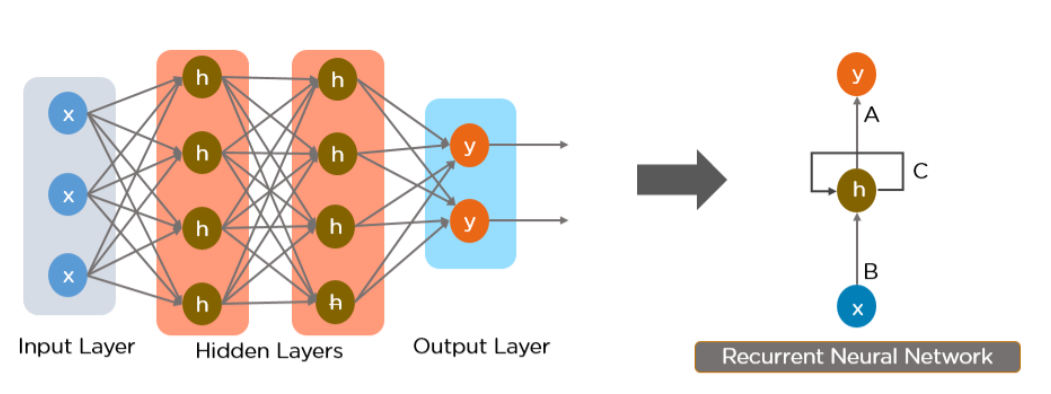
\includegraphics[scale=0.15]{rnn1}
    \caption{RNN visualised }
\end{figure}
\begin{figure}[h]
    \centering
    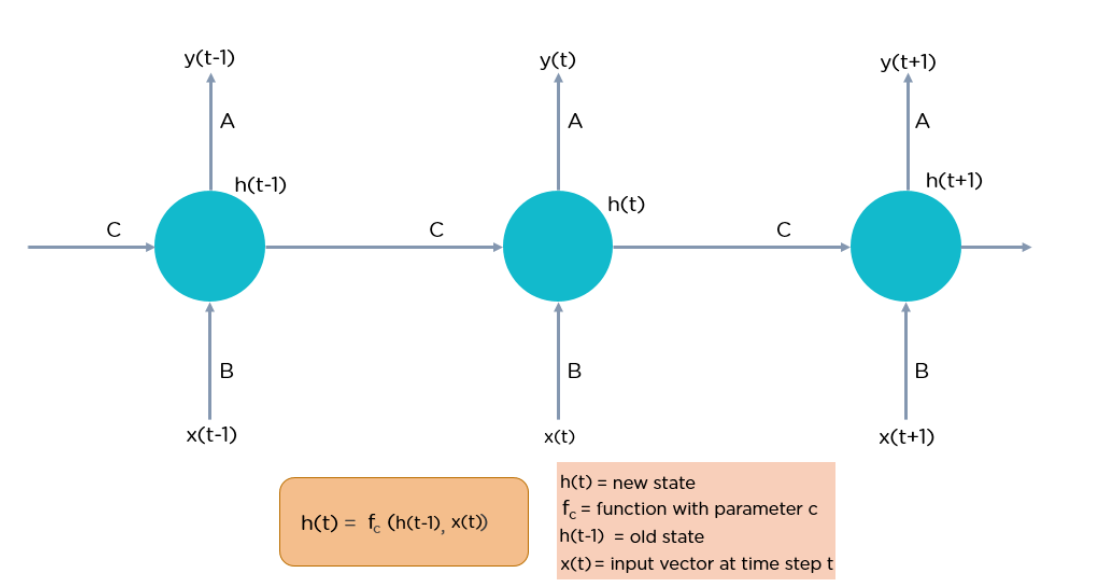
\includegraphics[scale=0.15]{rnn2}
    \caption{RNN broken down into individual components }
\end{figure}
\begin{figure}[h]
    \centering
    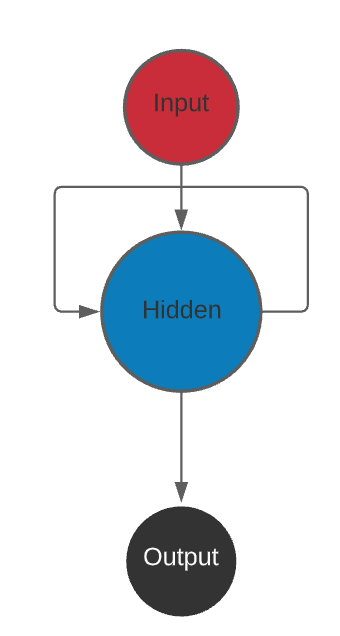
\includegraphics[scale=0.15]{rnn3}
    \caption{Individual block}
\end{figure}
\subsubsection{Problems with RNN}
The RNN has two big problems: a vanishing gradient problem and an exploding gradient
problem.\\
As previously mentioned, the gradient descent algorithm finds the minimum of a function to
find the optimal weights.\\
In RNNs, information first travels through time which means that information from previous
time points is used as the input for the next time points. Secondly the cost/error function is
calculated at each time point.\\
Essentially, every single neuron that participated in the calculation of the output, associated with
this cost function, should have its weight updated in order to minimize that error. And the thing
with RNNs is that it’s not just the neurons directly below this output layer that contributed but
all of the neurons far back in time. So, you have to propagate all the way back through time to
these neurons.\\
The problem relates to updating wrec (weight recurring) – the weight that is used to connect the
hidden layers to themselves in the unrolled temporal loop.\
For instance, to get from xt-3 to xt-2 we multiply xt-3 by wrec. Then, to get from xt-2 to xt-1 we
again multiply xt-2 by wrec. So, we multiply with the same exact weight multiple times, and this
is where the problem arises: when you multiply something by a small number, your value
decreases very quickly.\\
As we know, weights are assigned at the start of the neural network with the random values,
which are close to zero, and from there the network trains them up. But, when you start with
wrec close to zero and multiply xt, xt-1, xt-2, xt-3, … by this value, your gradient becomes less
and less with each multiplication.\\
(Biswal, 2021)

\subsection{LSTM}
All RNNs have feedback loops to help them maintain the information in the memory while
training but to resolve the problems mentioned above, the LSTM was created.
Long-short term memory networks are a type of RNN that introduces the use of gates such as
input and forget gates which allow for better control of the gradient flow hence allowing a
better preservation of long-range dependencies. These gates use functions that we have
mentioned before such as the tanh function, and the sigmoid function.
\begin{figure}[H]
    \centering
    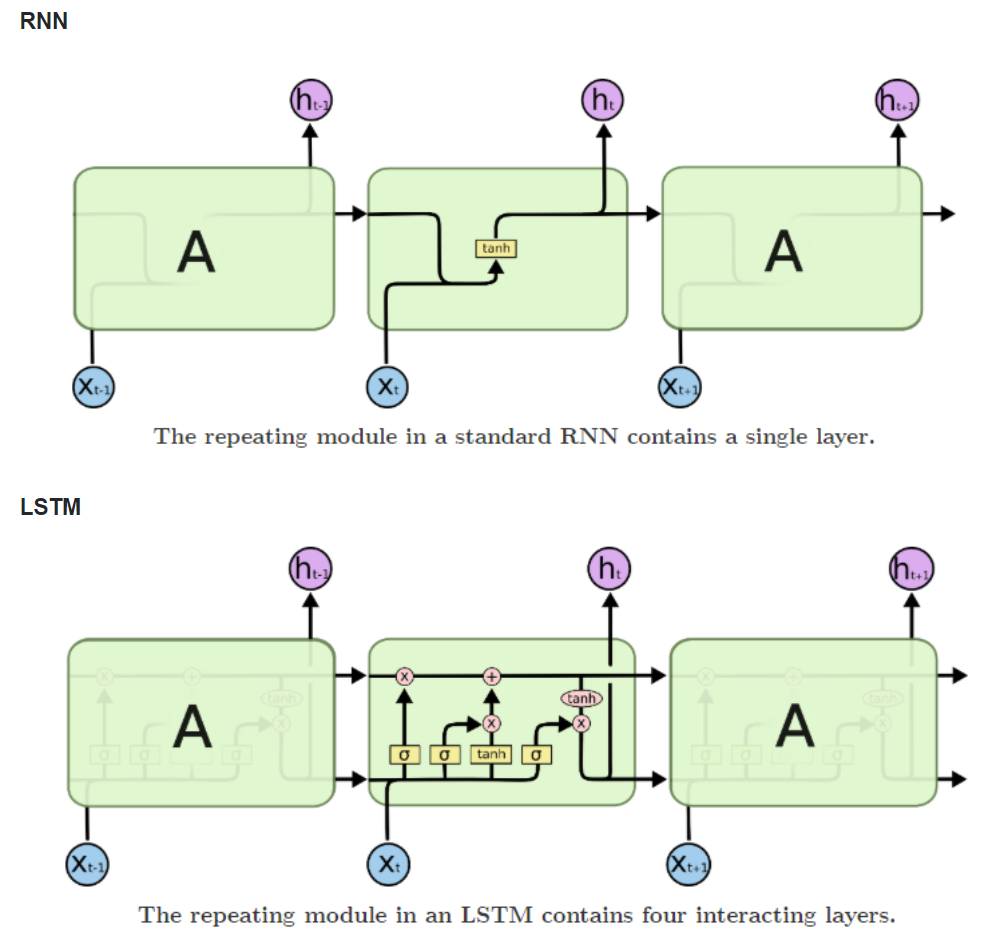
\includegraphics[scale=0.3]{lstm1}
    \caption{}
\end{figure}
(Olah,2015)
The LSTM has a block called the cell state, the middle block in the diagram above. The network
has the ability to remove or add information to the cell state so that it can be accessed at a later
time. This cell state is protected by the mathematical functions so that it doesn’t get cluttered
with useless information
\subsubsection{Problems with LSTM}
As you can see from the image above, there is a sequential path from the oldest past cells to the
current ones. This sequential path is now more complex with the addition of forget gates. This
makes them very resource intensive and so requires an immense amount of memory. This makes
them very inefficient and so unsuitable for small devices such as home devices like Amazon
Echo or Apple home pods.\\
LSTMs also get affected by different random weight initialisations and hence act just like a normal
feed forward neural network with extra steps making them nearly useless. They much prefer
small weight initialisations.\\
Along with these problems, LSTMs are prone to overfitting and are difficult to apply dropout
algorithms to resolve this issue. To add to this list is the fact that LSTMs struggle to retain
information when handling larger datasets. They can handle sequences of 100s but not 1000s or above. This makes them unsuitable for tasks like stock prediction or neural language processing.

\subsection{Transformers}
The Transformer is an evolution of the RNN and its main purpose was to solve the problem of
parallelisation. It only performs a small, constant number of steps. In each step it applies a
self-attention mechanism that helps it retain information for longer making it more suitable for
larger datasets. This model is typically used for neural language processing where keeping a
track of all the words used helps the machine to gain understanding about the context. A
common neural network would typically contain an encoder that would read the input sentence
and would generate a representation of it. A decoder would then generate the output sentence
while looking back to the representation the encoder created. The Transformer takes a different
approach; it starts by generating initial representations/embeddings for each word. A self
attention mechanism is then applied to the representation which generates a new representation
for the word by comparing it to previous words. This step of making a new representation is
repeated multiple times in parallel for all the words in the input sentence.\\
This parallelisation increases its computational performance and produces a high accuracy.
\begin{figure}[H]
    \centering
    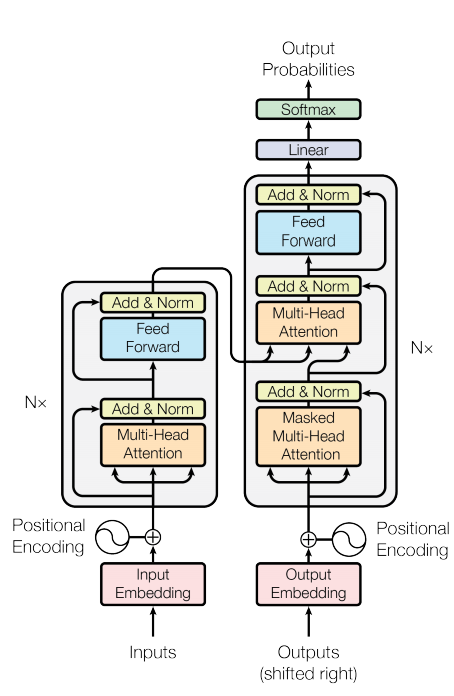
\includegraphics[scale=0.45]{transformer1}
    \caption{transformer model}
\end{figure}
(Vaswani et al., 2017)

\subsection{Attention}
(Lambda, 2019)
A critical and apparent disadvantage of this fixed-length context vector design is the incapability
of the system to remember longer sequences. Often it has forgotten the earlier parts of the
sequence once it has processed the entire sequence. The attention mechanism was born to resolve
this problem.\\
A neural network is considered to be an effort to mimic the brain in a simplified manner. The
attention mechanism can be described as an attempt to mimic the action of selectively
concentrating on a few relevant things instead of everything. There are two types of attention:
general attention and self-attention. General attention is between the input and output elements
and self-attention is within the input elements\\
The central idea behind attention is not to throw away any intermediate encoder states in LSTMs
and Transformers. Instead these states are used to construct the context vectors required by the
decoder to generate the output sequence.\\
A look into how self attention is calculated using vectors.\\
The first step in calculating self-attention is to create 3 vectors from each of the encoder’s input
vector, a query \boldsymbol{q}, a key \boldsymbol{k} and a value \boldsymbol{v}.\\
The second step is to calculate a score. The score determines how much focus to place on other
parts of the input as the input is encoded at a certain position.\\
The score is calculated by taking the dot product of the query vector with the key vector of the
respective value we are scoring. So if we are processing the self attention for the value in position
1 then the first score would be the dot product of $q_1$ and $k_1$. The second score would be the dot
product of $q_1$ and $k_2$.\\
The third step is to divide the scores by the square root of the dimension of the key vectors used.
This leads to having a more stable gradient.\\
This value will then be passed through the softmax function. This helps normalise the scores so
that they are all positive and add up to 1.\\
The fifth step is to multiply each value vector by the softmax score (in preparation to sum them
up). The intuition here is to keep intact the values of the word(s) we want to focus on, and
drown-out outliers (by multiplying them by tiny numbers like 0.001, for example).
The sixth step is to sum up the weighted value vectors. This produces the output of the
self-attention layer at this position for the first value.
\clearpage
\subsection{Temporal Fusion Transformers}
(Lim, 2020)
Attention is very useful for natural language processing but when handling time series data,
modifications have to be made. The temporal fusion transformer is the evolution made for this
type of data.
\begin{figure}[h!]
    \centering
    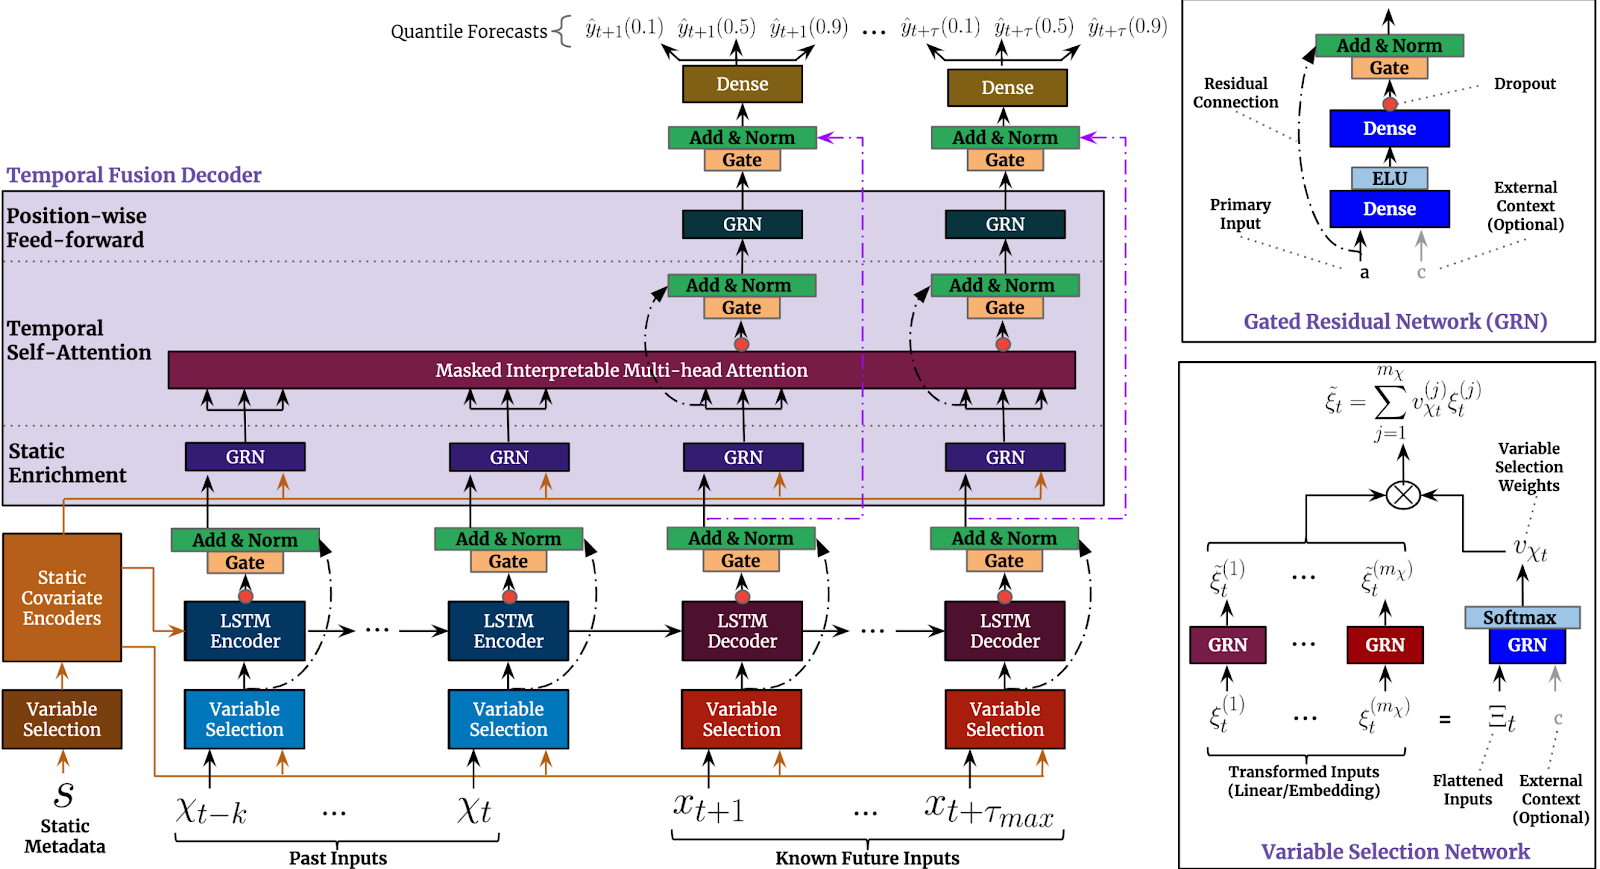
\includegraphics[scale=0.27]{tft}
    \caption{Temporal Fusion Transformer broken down into its components}
\end{figure}
The TFT has 5 main parts that get you from a dataset to a prediction. These allow the TFT to
efficiently predict future data points with a high performance.
\begin{enumerate}
\item Variable selection networks are used to select relevant input variables at each time step.
\item The gating mechanism to skip over any unused blocks and components of the architecture to allow for a dynamic model that adjusts itself to account for the dataset hence making it more time and memory efficient. This helps accommodate for larger datasets as well making the model more versatile.
\item The static covariate encoders are used to integrate start features into the network by encoding context vectors to condition temporal dynamics.
\item Temporal processing is used to learn both short and long term relationships between past and current inputs. Here a sequence to sequence layer with a multi-head attention block.
\item Prediction intervals via the forecasts to calculate the range of likely values at each step.
\end{enumerate}

\subsection{Tensors}
An $n$th-rank tensor in $m$ dimensional space is a mathematical object that has $n$ indices and $m^n$ components that obeys certain transformation rules

\subsubsection{Tensor Product}
For any two vector spaces $\vec{U}$,$\vec{V}$ over the same field $F$, we can construct a tensor product $\vec{U}\otimes\vec{V}$ which is also an F-vector space.\\
Example:
$$\vec{v}=\begin{pmatrix}1\\ 2\\ 3\end{pmatrix}\quad \vec{w}=\begin{pmatrix}4\\ 5\end{pmatrix}$$
V is a vector in $\mathbb{R}^{2}$. W is a vector in $\mathbb{R}^{3}$.
$$\vec{v}\otimes\vec{v} \rightarrow \begin{pmatrix}1\cdot 4\\ 1\cdot \:5\\ 2\cdot \:4\\ 2\cdot \:5\\ 3\cdot \:4\\ 3\cdot \:5\end{pmatrix}=\begin{pmatrix}4\\ 5\\ 8\\ 10\\ 12\\ 15\end{pmatrix}$$

\subsection{Gated Linear Units(GLU)}
GLUs can be defined by the following equation:
$$h(x)=(x\cdot W +b)\otimes \sigma(X\cdot V+c)$$
Given a tensor, two independent convolutions are done and we get two outputs. We further do an additional sigmoid activation for one for the output, and find the tensor product of the two outputs.


\subsection{Gated Residual Network(GRN)}
\begin{figure}[H]
    \centering
    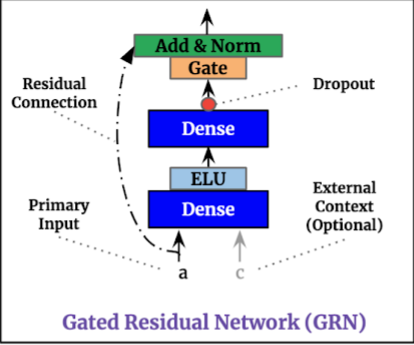
\includegraphics[scale=0.45]{grn}
    \caption{GRN visualised}
\end{figure}

The gated residual network, as shown in the image above,  consists of a dense block with an exponential linear unit as the activation function. This is then fed into another dense block before a GLU and normalised. There will be a connection between the input and output to allow for the attention mechanism to work. In my model, there will not be external context. The GRN can be modelled using the equations below:
$$GRN(\alpha) = LayerNorm(\alpha + GLU(\phi_1)) $$
$$\phi_1 = W_1, \phi_2+b_1$$
$$\phi_2 = ELU(W_2, \alpha + W_3) $$
$$\phi_1,\phi_2\in R $$

\subsection{Variable Selection Network}
\begin{figure}[h]
    \centering
    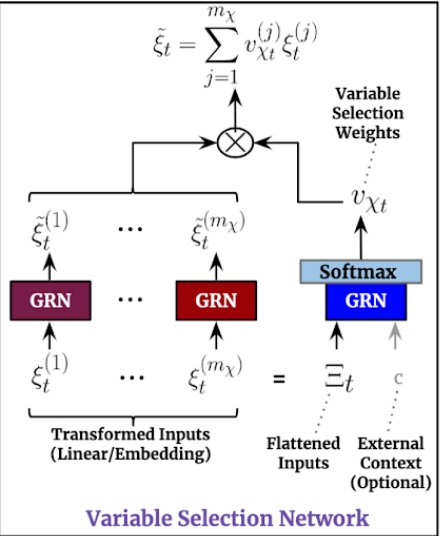
\includegraphics[scale=0.45]{vsn}
    \caption{Variable Selection Network visualised}
\end{figure}

The purpose of the variable selection network is to evaluate the relevance of the variables than can be fed back into the model. This helps tell us what variables are the most significant as well as removing any unnecessary, noisy inputs that could negatively impact the performance of the model. This is useful when dealing with real time data as there might not be enough time to make sure all the data is correct or useful. As shown in the image above, there will be three GRNs with one of them having a softmax as the activation function. The tensor product will then be calculated.

\subsection{Multi-head attention}
The TFT model uses a self-attention mechanism to learn long term relationships between the data points across the different time steps. The concept of attention has already been explained and how that is calculated has also been discussed. To fit the TFT, a few modifications have been made. The general self-attention relies on the head value being the same but in our case this is different. This means the attention mechanism would have to only rely on the attention weights which is not enough. This problem has been solved by modifying the multi-head attention to share values in each head and using additive aggregation of all the heads.

$$MultiHead(\vec{Q},\vec{K},\vec{V}) = [\vec{H_1},...,\vec{H_h}]\cdot\vec{W_h} $$
$$ \vec{H_h}= Attention(\vec{Q}\vec{W_Q},\vec{K}\vec{W_K},\vec{V}\vec{W_V})$$
$$InterpretableMultiHead(\vec{Q},\vec{K},\vec{V})=\vec{\tilde{H}}\cdot\vec{W_H}$$
$$ \vec{\tilde{H}}=\tilde{A}(\vec{Q},\vec{K]})\cdot\vec{V}\vec{W_V}$$
$$=\frac{1}{H}\sum _{h=1}^{M_h}Attention(\vec{Q}\vec{W_Q},\vec{K}\vec{W_K},\vec{V}\vec{W_V})$$
The first equation shows what the equation would be when multiple heads are added. Q,K and V are the query vectors, key vectors and value vectors. Wv are the value weights shared across all the heads.
The interpretable multi-head function is our modified equation. The last equation shows us how we have employed additive aggregation.

\subsection{Quantile Forecasts}
The TFT can generate prediction intervals as well as point forecasts. This is done by predicting various percentiles (10\%, 50\%, 90\%) at each time step. The quantile forecast is calculated using the outputs of the temporal fusion decoder as is written as this:
$$\tilde{\xi} = GRN(\xi)$$
$$\phi(t,n)=LayerNorm(\tilde{\xi}+ GLU(\phi(t,n)))$$
$$\psi(t,n)= LayerNorm(\phi(t,n)+GLU(\psi(t,n)))$$
$$\hat{y}(q,t,n)=\vec{W_q}\psi(t,n)+b_q$$
The equations above shows us what is being calculated to end up with the last equation which is our quantile forecast.


\subsection{Software}

\subsubsection{Coding Language}
I have chosen to use python to code my project due to a few reasons. The first reason is the flexibility of the language. I have the option to use OOP and functional programming as well as not having to recompile the code every time I want to run the code. Python can also be combined with other languages such as C which makes it more powerful when dealing with a lot of maths.
Another reason is that Python has a very big library for machine learning. This makes prototyping and implementing my own algorithm a lot easier as well as being able to visualise my code a lot easier with packages such as pyplot.
My other option was C/C++ where I would’ve had benefits such as more compact and faster runtime. Python does offer extensions or libraries that optimise the Python code. An example is Theano. Unlike C++ where specific optimisations need to be made, Python can run nearly any system without any time being wasted on specific configurations. Python also has access to libraries such as CUDA python. Libraries like that are made to help with parallelisation on GPUs. This exploits the tensor cores that are offered by the hardware manufacturers. The power to be able offload tasks to the GPU makes any performance advantage C++ had, instantly insignificant.
GIE is the NVIDIA GPU inference engine.
\begin{figure}
    \centering
    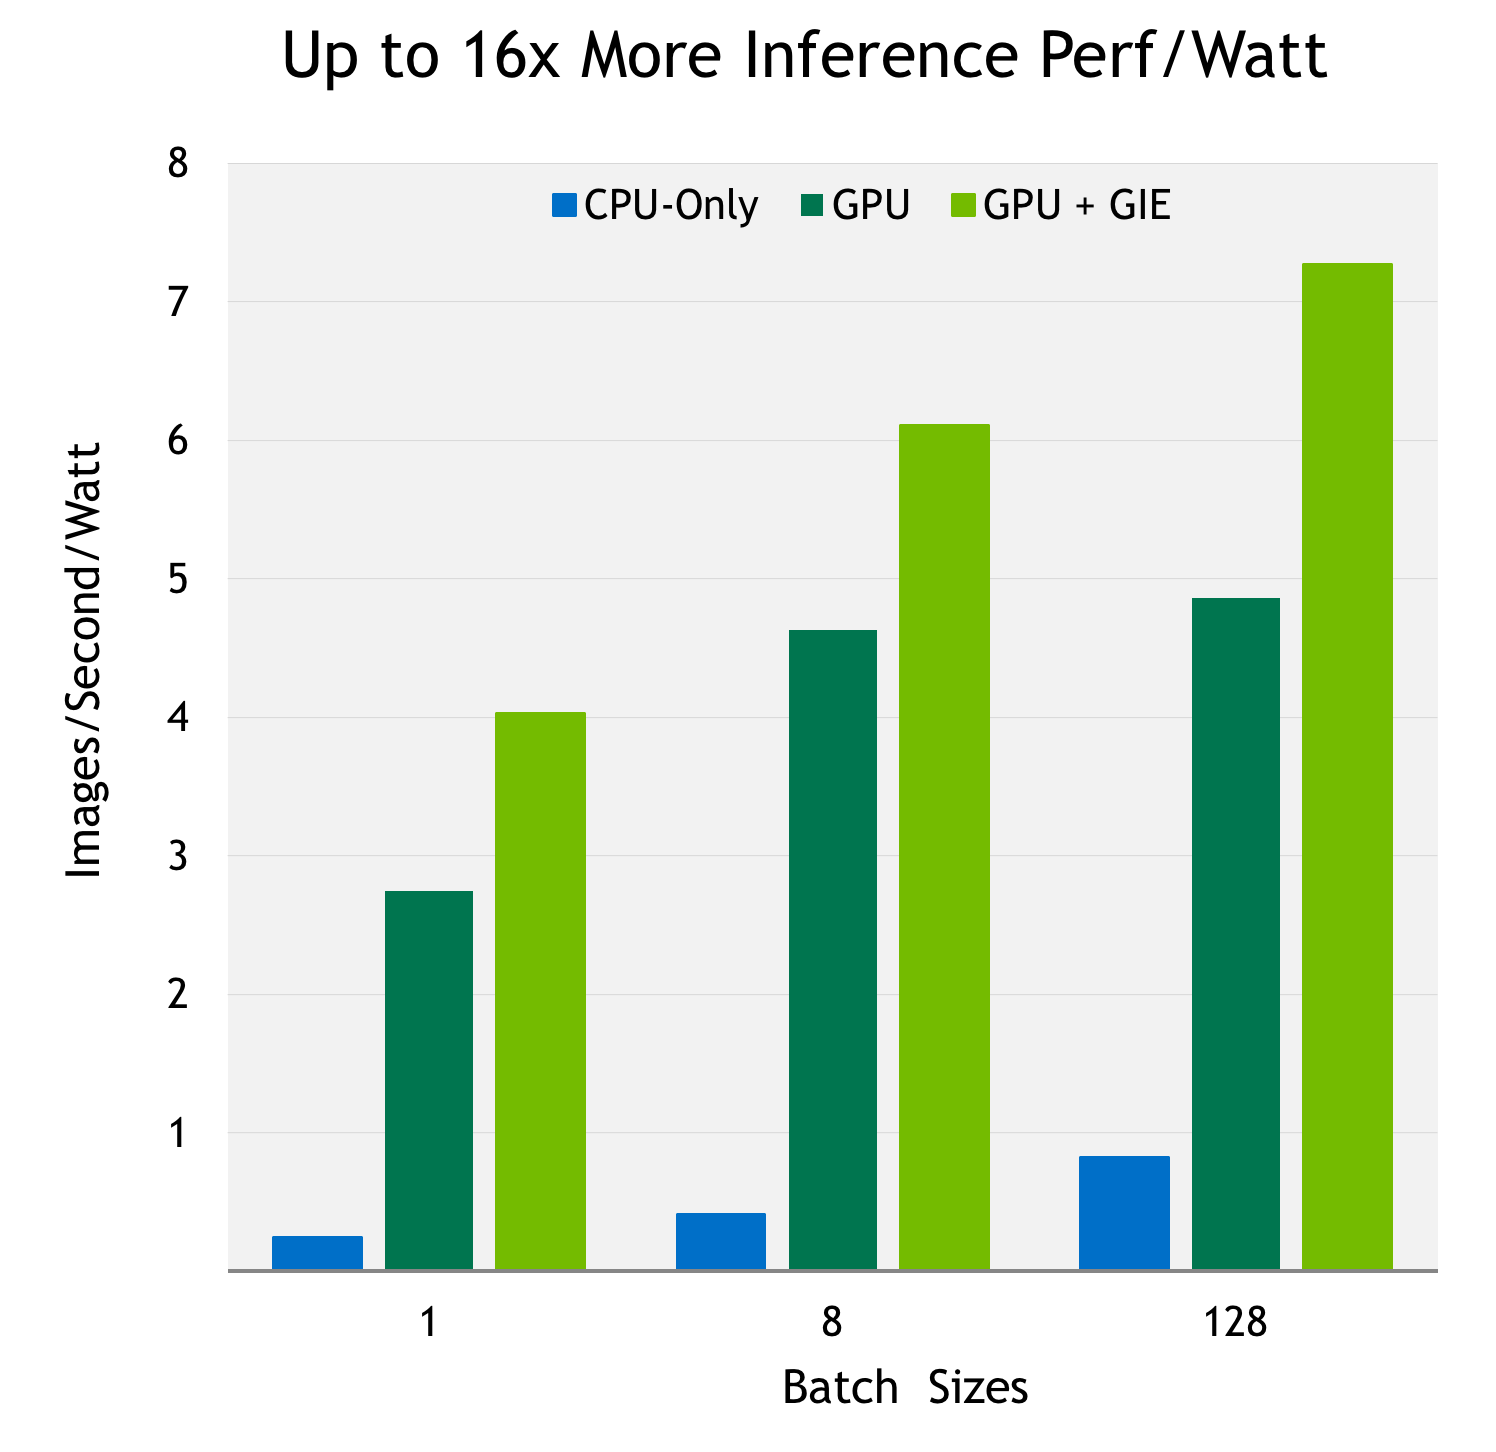
\includegraphics[scale = 0.15]{software1}
    \caption{}
\end{figure}
\begin{figure}
    \centering
    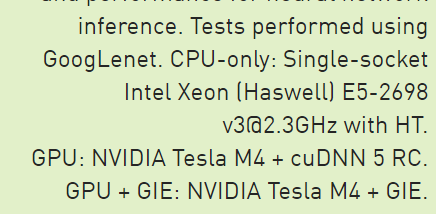
\includegraphics[scale = 0.15]{software2}
    \caption{}
\end{figure}
The graph shows the advantage GPUs provide for training deep learning models.

\subsubsection{Packages}
For my project I have considered using packages to aid the learning process such as Theano. Theano is a CPU and GPU mathematical compiler that outperforms other tools. Theano includes tools for manipulating and optimising graphs representing mathematical functions. An example is the sigmoid function that is used heavily in machine learning. Theano’s optimisation also includes the elimination of duplicates or unnecessary computations therefore increasing the numerical stability as well as increasing speed.  The graph representation allows the user to quickly prototype machine learning models as the differentiation of the function does not have to be calculated in algorithms such as backpropagation. This reduces the amount of code that has to be executed. Theano also uses CUDA to define a class of n-dimensional arrays located in GPU memory with Python bindings. This speeds up the number of operations that are performed per second. Theano can also leverage multi-core CPU architectures to allow for parallelisation on both the CPU and the GPU. Some disadvantages of using Theano include the speed of compiling is a lot larger with bigger models. The error messages are also difficult to understand which will make debugging harder. Theano is a quite low level so the learning curve is steeper.
Another package that I could use is Tensorflow. Tensorflow has a flexible architecture and can be deployed on more than one GPU or CPU. As well as this it shares all the features that Theano has. The reason I am not using it is because it is very high level and does not give you enough control at the base layer.

\subsection{Objectives}
The aim of this project is to be able to make predictions on the price of a stock given historic data of the stock.
\\
\subsubsection{General Objectives}
\\
Data processing
\begin{enumerate}
    \item Must be able to accept a CSV file as an input
    \item Must normalise the data set
\end{enumerate}

Prediction
\begin{enumerate}
    \item Must pass the data through a variable selection block
    \item Must pass the data through an LSTM encoder
    \item Must pass the data through a series of GRNs
    \item Must implement multi head attention
    \item Must return quantile forecasts
\end{enumerate}

Forecast processing
\begin{enumerate}
    \item  Extra - decide whether to recommend a sell, short or buy
    \item  Extra - calculate the confidence level of the forecast
\end{enumerate}

User interface
\begin{enumerate}
    \item Extra - display the forecast along with a confidence level
    \item Extra - give recommendations for buying, shorting or selling
    \item Consider giving alerts to help the user
\end{enumerate}

\subsubsection{Specific objectives}

Gated Residual network
\begin{enumerate}
    \item Must have a dense network
    \item Must have an exponential linear unit
    \item Must have layer normalisation
    \item Must have a residual connection between the input and output
\end{enumerate}
Variable Selection block
\begin{enumerate}
    \item Must have three GRNs
    \item Must have a GRN with a softmax function
    \item Must calculate the tensor product of the three GRNs
\end{enumerate}
LSTM encoder-decoder
\begin{enumerate}
    \item Must have an encoder model
    \item Must have a decoder model
    \item Must have a dense block
\end{enumerate}
Multi-head attention
\begin{enumerate}
    \item Must take the embedding size, the query size and attention heads as an input
    \item Must have input embedding and position encoding layers to produce a matrix of shape
    \item The matrix must be fed to the query, key and value of the first encoder in the stack
    \item The input must be passed through linear layers to produce the Q, K and V matrices
    \item The data must get split across the attention heads
    \item The Q, K and V matrices must be reshaped
    \item An attention score must be computed for each head
    \item The attention scores must be merged together
\end{enumerate}

\subsubsection{Extension Objectives}
Real-time Data
\begin{enumerate}
    \item Ingestion layer
    \item Managing message buses and streams using Azure Service Bus
    \item Processing layer using Apache Storm
    \item Stream querying using Azure Stream analytics
    \item Decision engine using stateless engines such as Gandalf
\end{enumerate}


\clearpage
\section{Documented Design}
\subsection{Hierarchy Diagrams}
The project can be split into 3 main sections: data pre-processing, the temporal fusion transformer model and the quantile forecasts.
\begin{figure}[H]
    \centering
    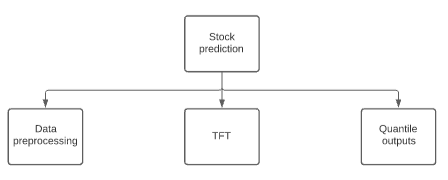
\includegraphics[scale = 0.4]{hd1}
    \caption{}
\end{figure}
Data processing can also be split into 3 parts: Processing, normalisation and adding time embeddings.
\begin{figure}[H]
    \centering
    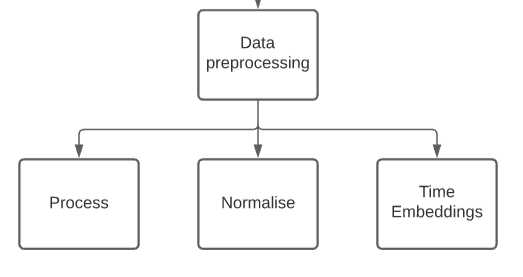
\includegraphics[scale = 0.4]{hd2}
    \caption{}
\end{figure}
Below is a structure diagram of the Temporal Fusion Transformer. It is split into 4 sections: Gated Blocks, LSTM, Variable Selection Network and Multi-head Attention. Each of those sections are further subdivided into the different types of that object.
\begin{figure}[H]
    \centering
    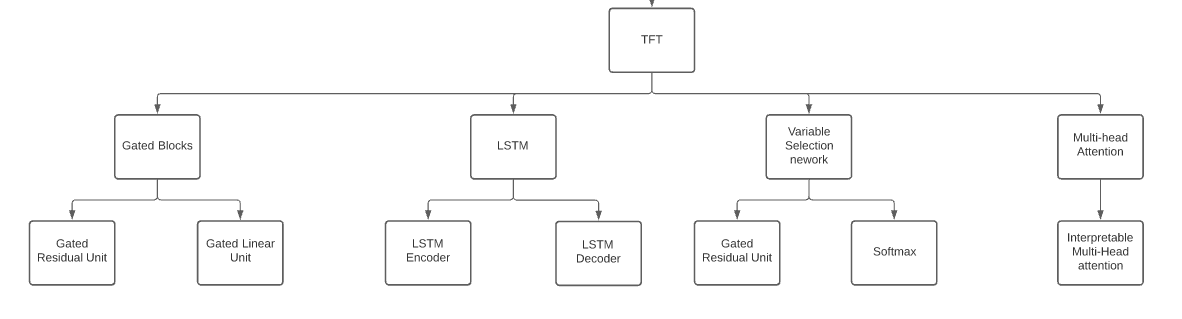
\includegraphics[scale = 0.35]{hd3}
    \caption{}
\end{figure}
The Quantile outputs are split into functions that are used in the main TFT model, layer normalisation, GRU and GLU. These together will form the forecasts at the end.
\begin{figure}[H]
    \centering
    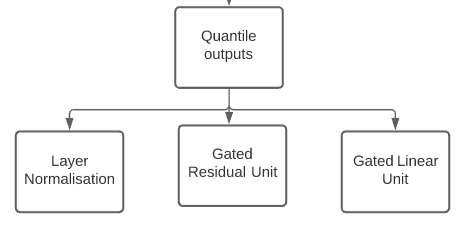
\includegraphics[scale = 0.4]{hd4}
    \caption{}
\end{figure}
The Gated Residual unit can be broken up into 3 parts: the dense network, the exponential unit and the addition and normalisation layer.
\begin{figure}[H]
    \centering
    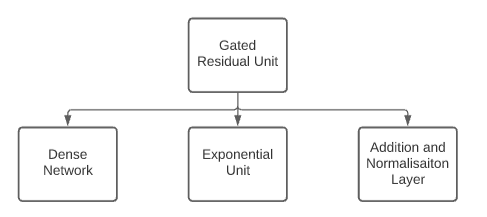
\includegraphics[scale = 0.4]{hd5}
    \caption{}
\end{figure}

\clearpage
\begin{figure}[H]
    \centering
    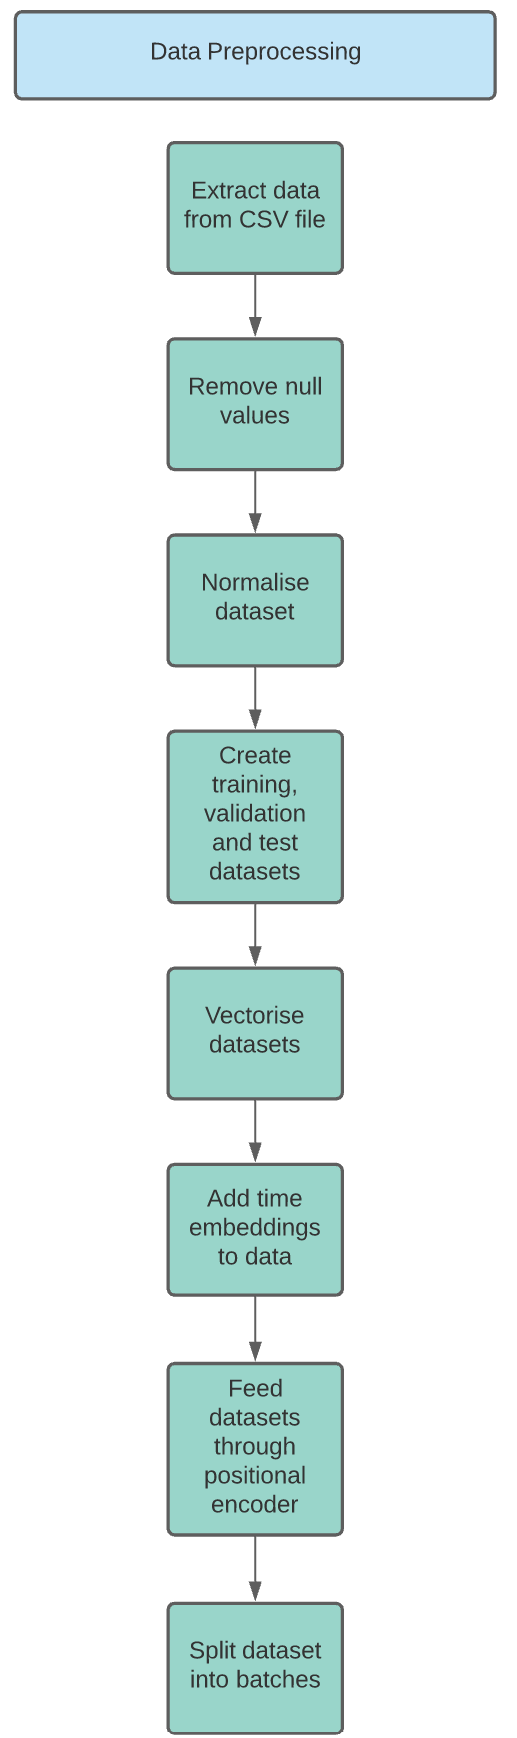
\includegraphics[scale = 0.5]{hd6}
    \caption{}
\end{figure}
This figure shows an overview of the Data Pre-processing. This part of the program will ensure that all the data is fit to be fed to the model and will convert the values into a form that is best for the machine learning module(TFT). This process includes removing all null values, creating the appropriate datasets, vectorising them, adding time embeddings and then finally splitting the datasets into batches.
Removing null values will ensure that sudden spikes in the data do not add a bias to the model. A spike will have a big derivative and might cause the wrong neurons to be activated.
Normalising a dataset will ensure that all the data lies within 0n1. It is required as my data have different ranges. Having all values between the same range is needed to make sure larger values in a dataset don't have a greater importance/bias. This will help speed up the model as the calculations and multiplication will be done with smaller numbers. Rounding is acceptable as we are dealing with a machine learning model and not a statistical learning model. Rounding will not have a significant impact on the overall accuracy.
The dataset has to be split into 3 parts: the training dataset, the validation dataset and the testing dataset. The split will be roughly 80:5:15. It is important to make sure that the training data is not used when testing as this will give us an hyperinflated accuracy, making the model seem a lot better than it actually is.
The datasets then have to be vectorised as the model will only take in vectors, matrices or tensors.
Time embeddings are added to the data. This is to help the attention part of the model. Attention works by referring back to the previous data points and so each data point has to be given a time stamp/embedding.
The positional encoder will assign data points a value to determine their position in the dataset. This is also used to help make sure the attention module works,
The dataset will finally be split up into batches. This is so that I can conduct batch training. This helps the model focus on small sections of the data instead of trying to consider all the data at once. This helps the code be more memory efficient and will lead to a higher accuracy score.

\begin{figure}[H]
    \centering
    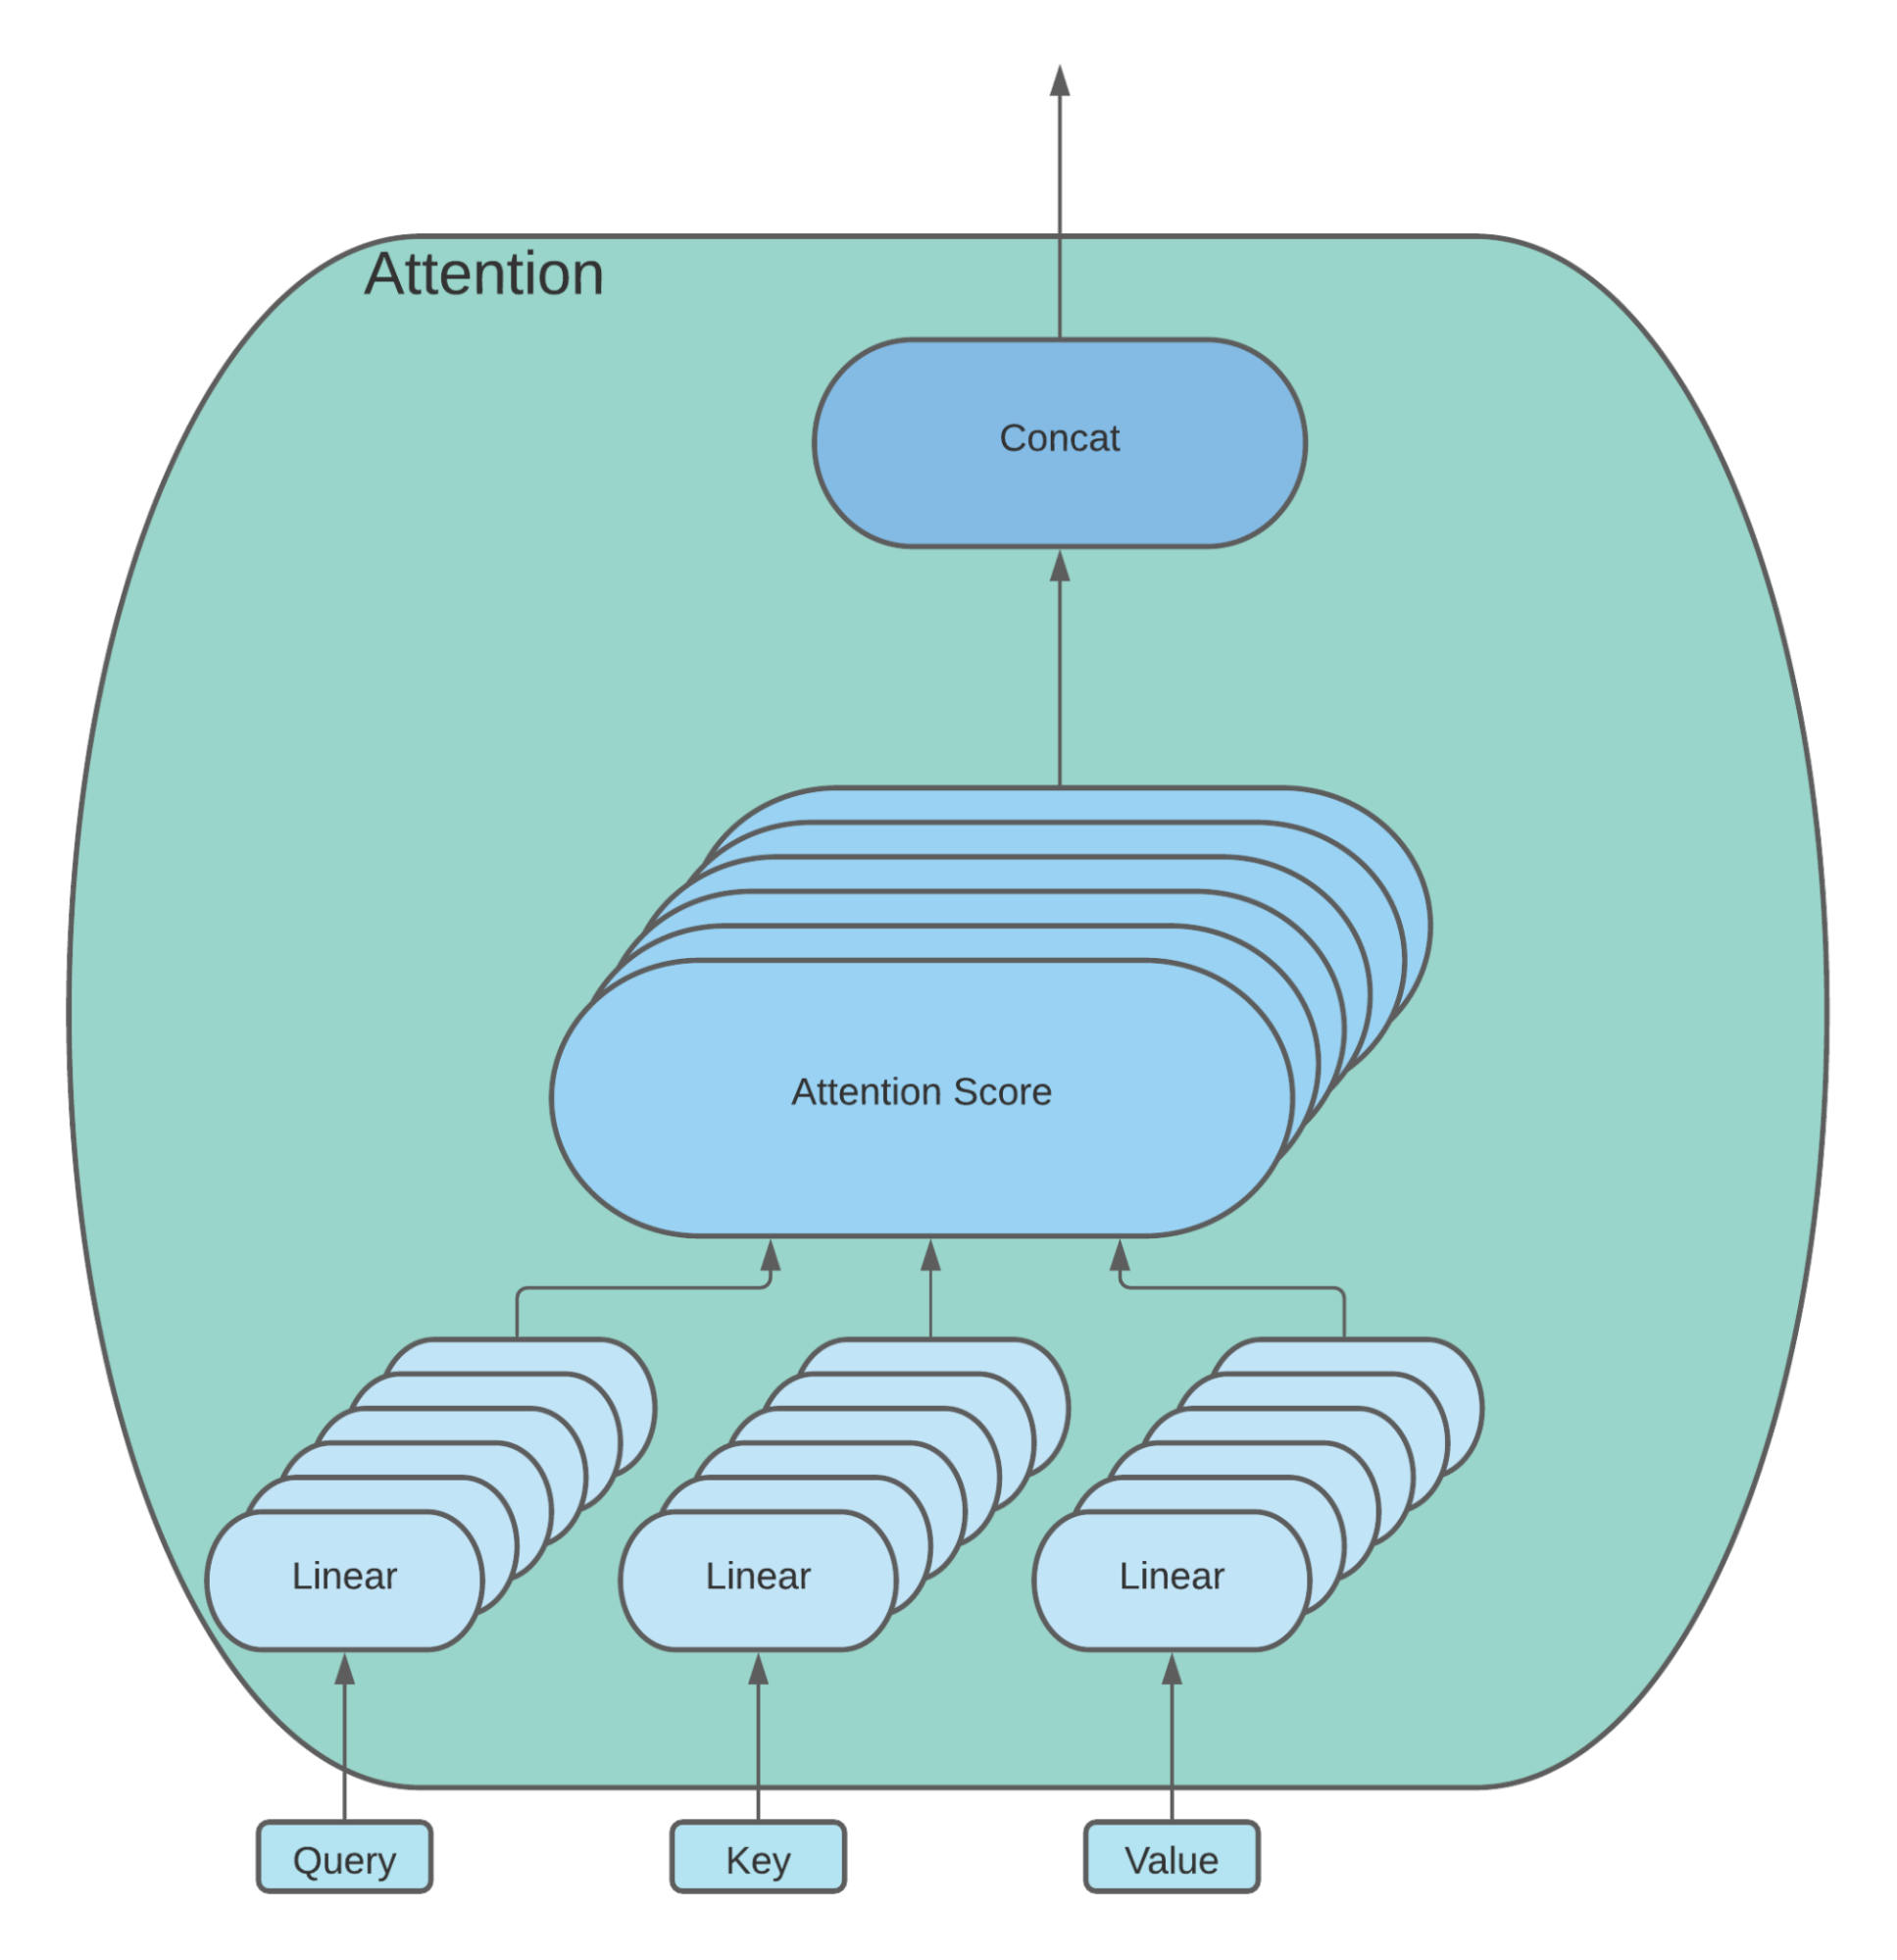
\includegraphics[scale = 0.15]{attention1}
    \caption{}
\end{figure}
The figure above shows how the attention mechanism works. The module takes in 3 input vectors: Query, Key and Value. These are fed into the attention block and an Attention score is calculated using the equation detailed in the analysis section. The multiple linear and attention score blocks represent the number of heads in the attention block.


\begin{figure}[H]
    \centering
    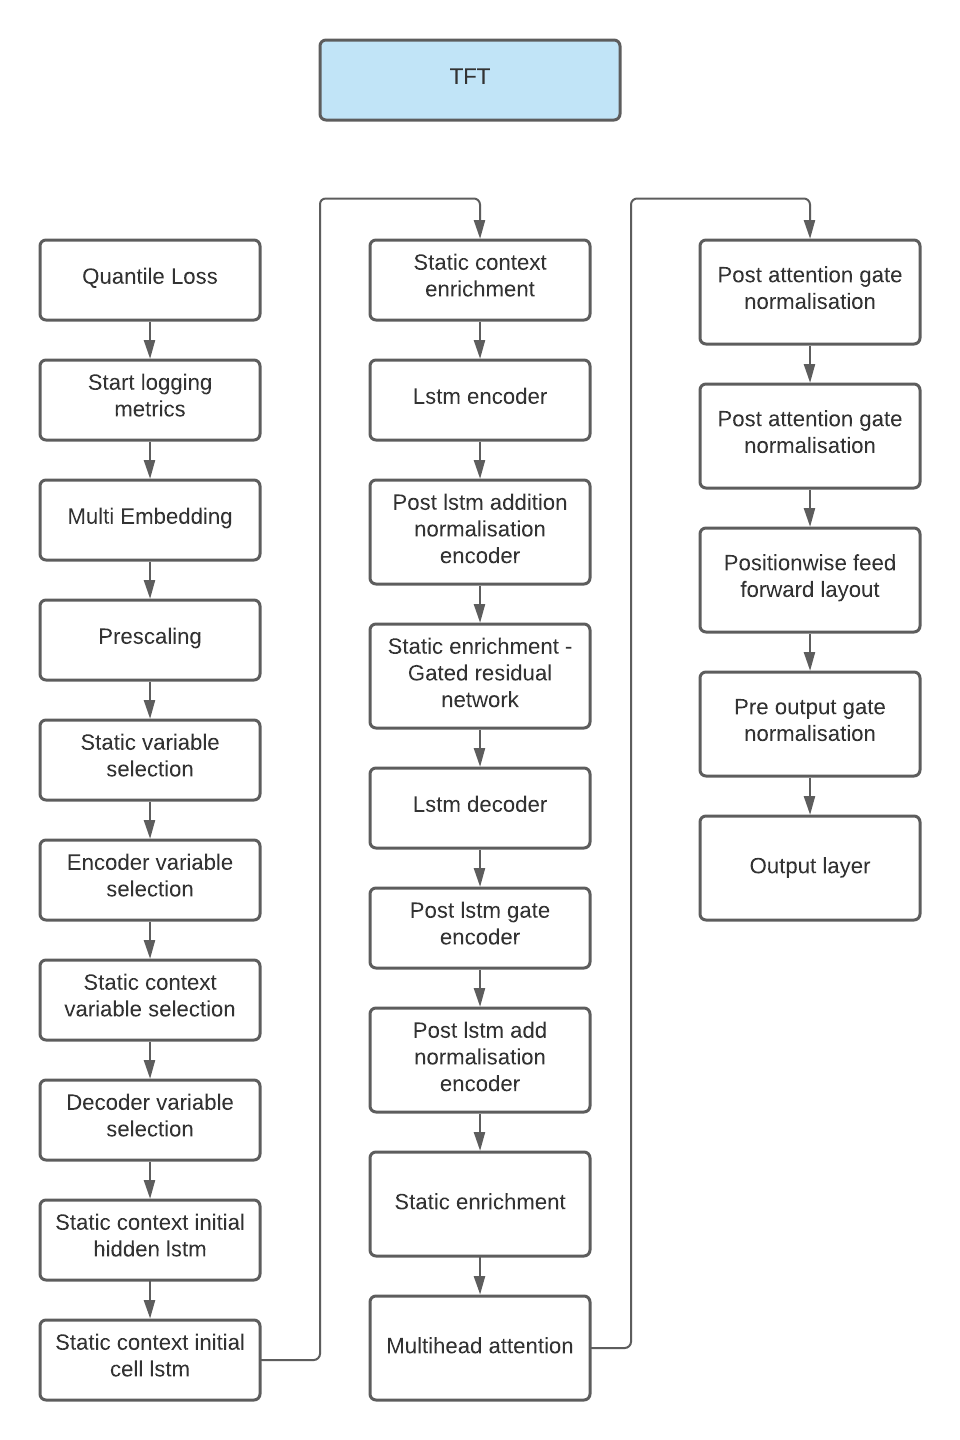
\includegraphics[scale = 0.4]{tft2}
    \caption{}
\end{figure}

Above is a flowchart to show the travel of data in my program. The TFT module starts off with the quantile loss and ends with the output layer.
The logging metric is going to be in the form of a tensorboard. This tracks important data such as the change in loss as the number of epochs increases. I can track and see the change in weights through the neural network. This helps me evaluate the performance of certain blocks in the TFT. The tensorboard will also allow me to compare different initialisation techniques such as truncated and xavier. The most important reason is to find out when to stop training the model. The graph of loss vs epoch can be thought of as a 1x graph for 0x. As the graph starts to level off, the net effect of each epoch decreases. Training a machine learning algorithm is time, space and cost intensive so any effort to reduce the number of epochs has to be taken. Analysing the graph provided by the tensorboard will allow this.
The main part of the machine learning model(TFT) aims to pass the data through many blocks that will analyse the overall trend in the data while observing patterns in the data. The use of LSTMs and Gated Residual Units contain memory blocks that help the neural network consider context. At the start there are encoders and so therefore later on decoders are required. Multihead attention is used later on to use attention to provide further context to the model.

\begin{figure}[H]
    \centering
    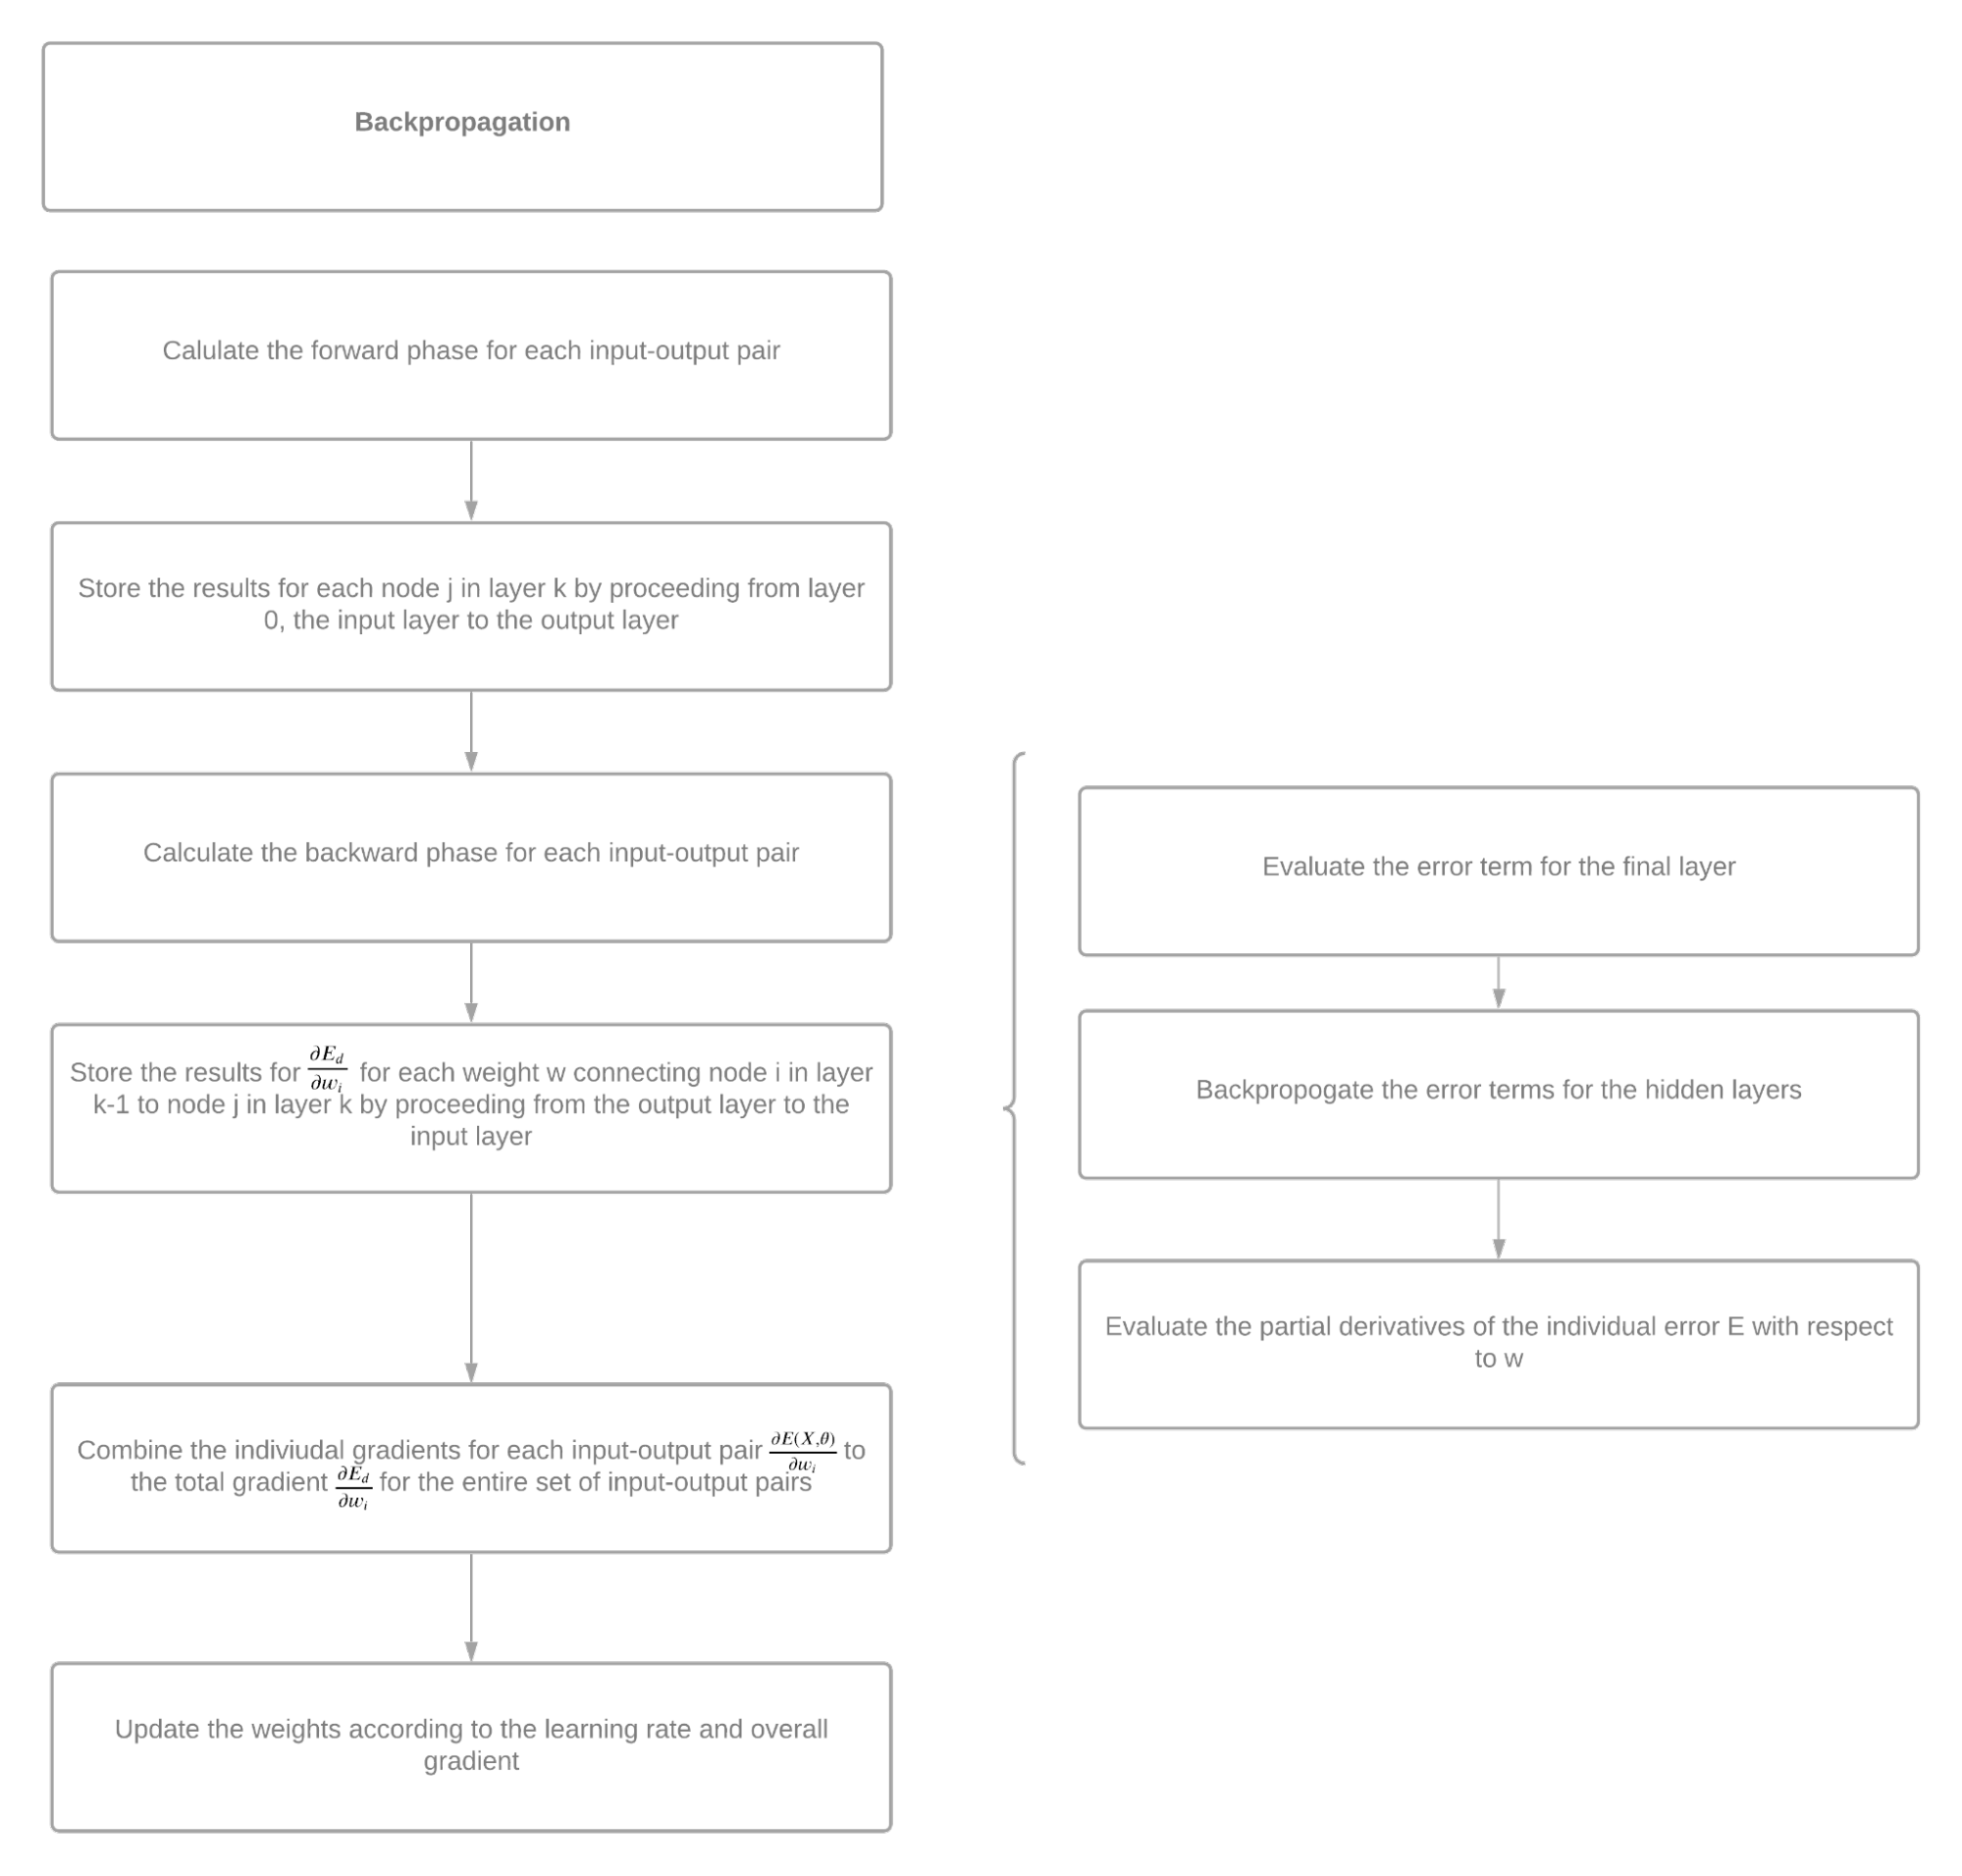
\includegraphics[scale = 0.24]{backprop1}
    \caption{}
\end{figure}

This figure illustrates how backpropagation will work. This is for a standard dense network, backpropagation is similar in LSTMs and other blocks but may not be the exact same.
The figure below shows the different modules.
\begin{figure}[H]
    \centering
    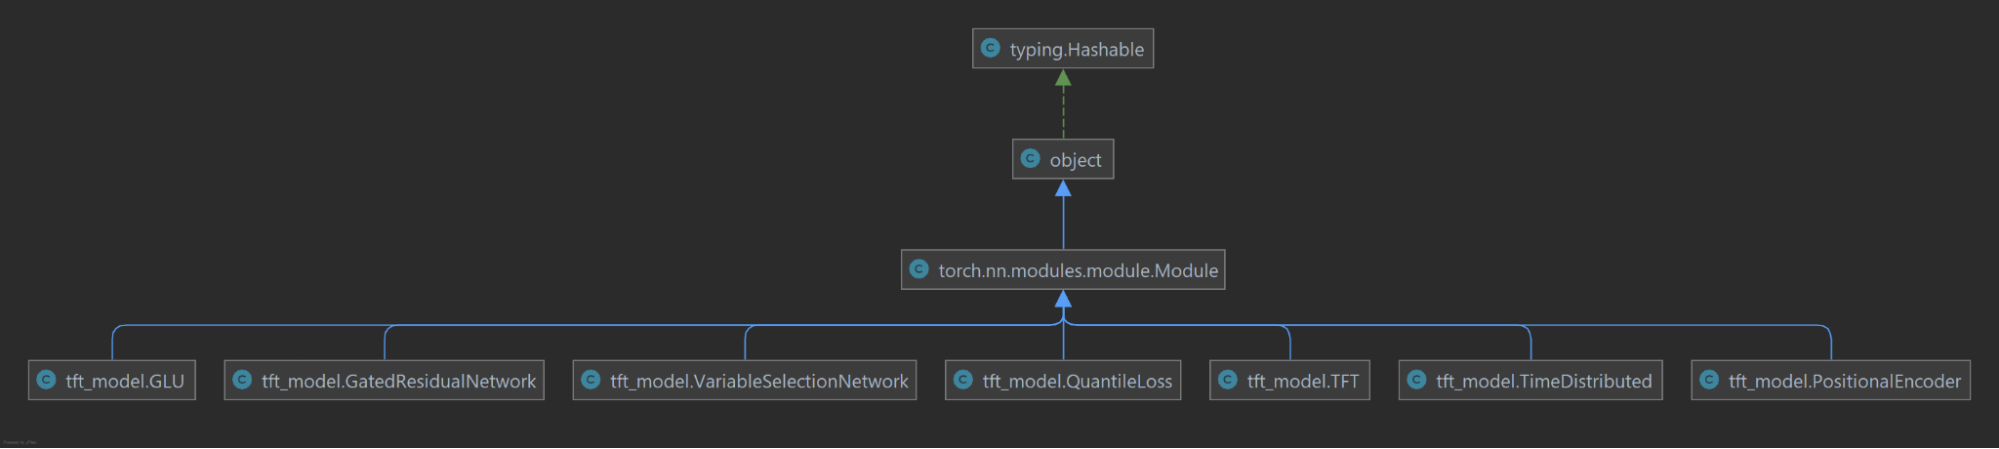
\includegraphics[scale = 0.45]{hd7}
    \caption{Hierarchy Diagram}
\end{figure}
\clearpage
\subsection{Class Diagrams}
Below are the class diagrams for the most complex classes. The letter m in red shows the methods and the f in yellow represents the functions.\\
In my implementation, attributes are inherited from the nn.Module class. This module contains basic functions and attributes that are needed to pass
layers and create specific modules. I have incorporated dynamic polymorphism as well as static polymorphism. This is most clear in the activation functions
class.
\subsubsection{Gated Linear Unit}
\begin{figure}[H]
    \centering
    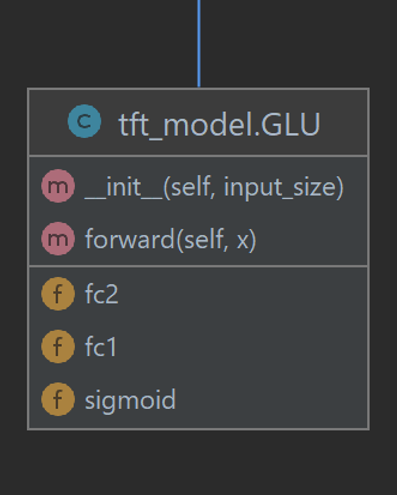
\includegraphics[scale = 0.6]{hd8}
    \caption{GLU}
\end{figure}
\subsubsection{Gated Residual Network}
\begin{figure}[H]
    \centering
    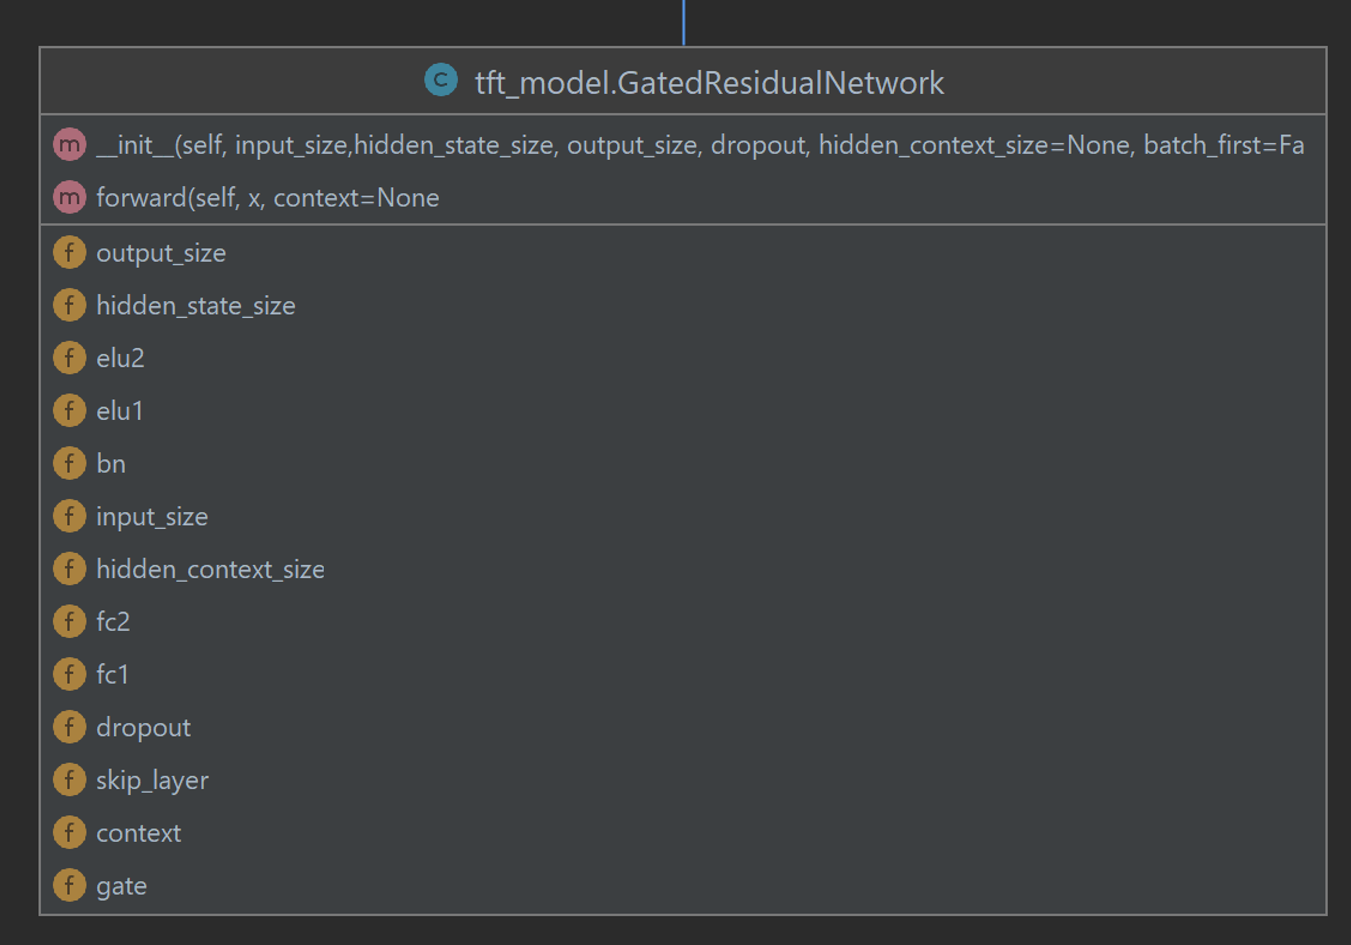
\includegraphics[scale = 0.315]{hd9}
    \caption{GRU}
\end{figure}
\subsubsection{Variable Selection Network}
\begin{figure}[H]
    \centering
    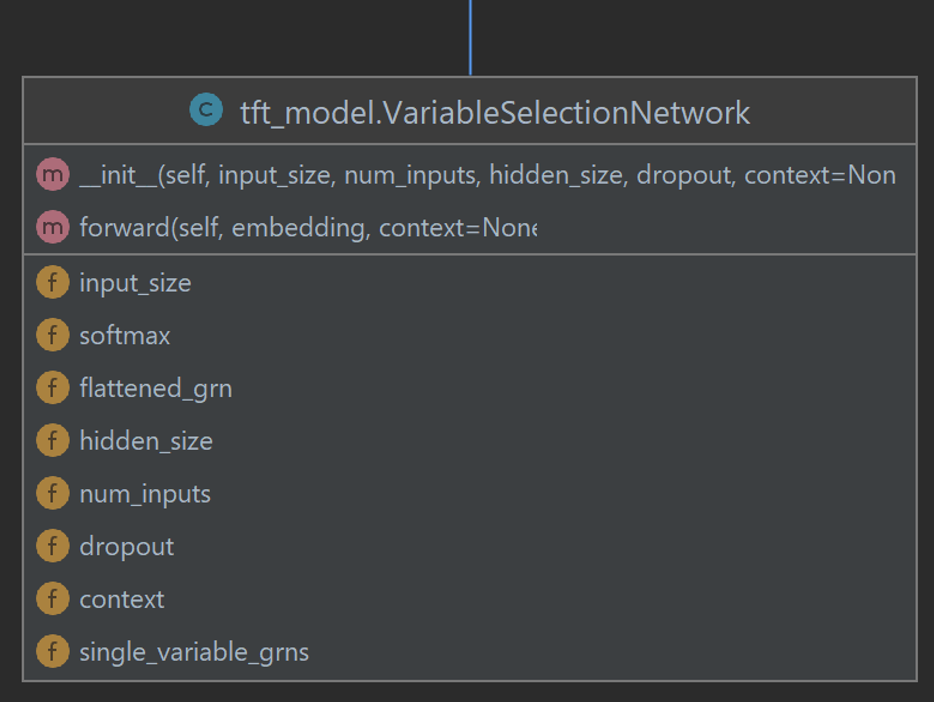
\includegraphics[scale = 0.5]{hd10}
    \caption{VSN}
\end{figure}
\subsubsection{Quantile Loss}
\begin{figure}[H]
    \centering
    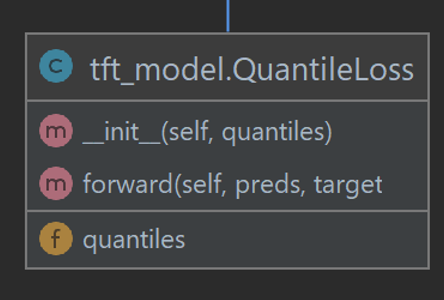
\includegraphics[scale = 0.5]{hd11}
    \caption{Quantile Loss}
\end{figure}
\subsubsection{Temporal Fusion Transformer}
\begin{figure}[H]
    \centering
    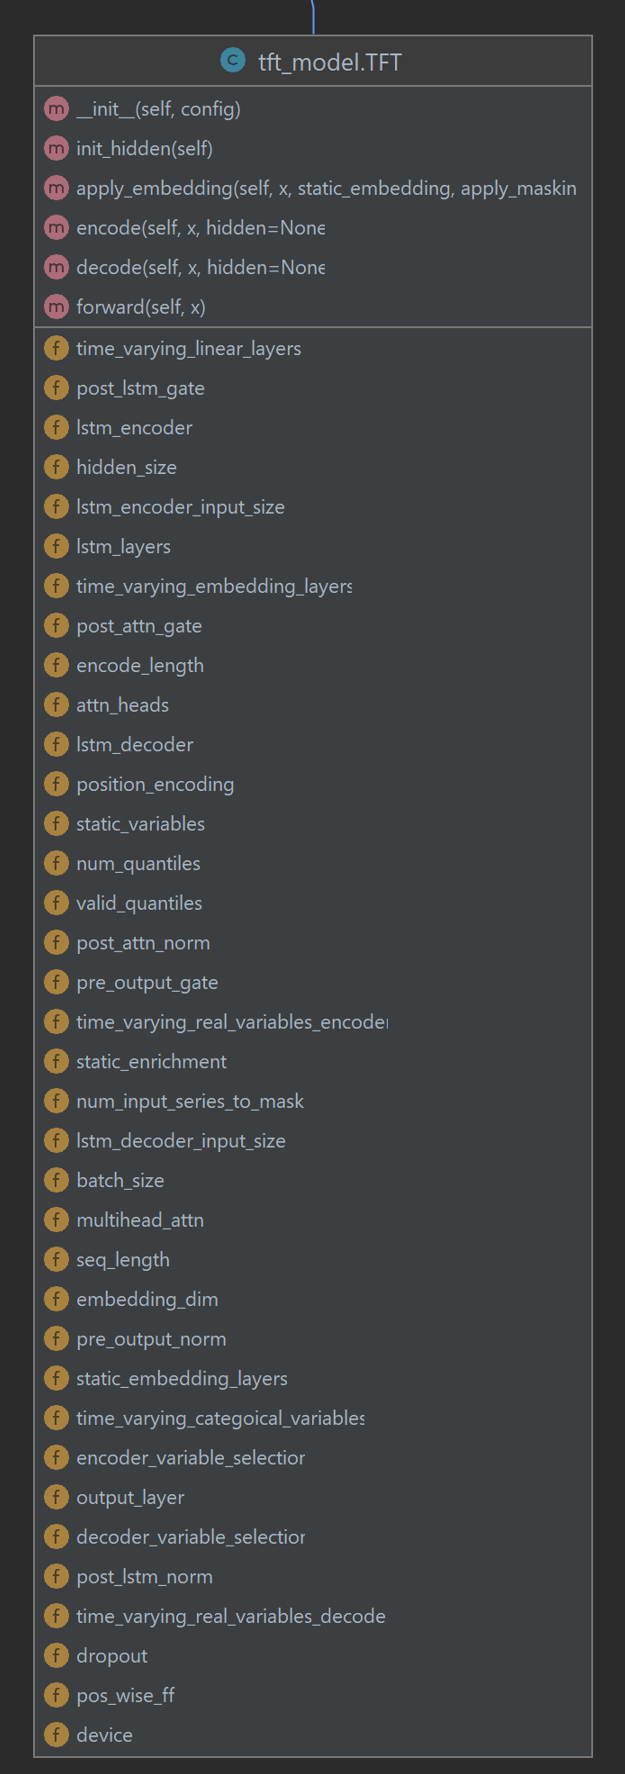
\includegraphics[scale = 0.5]{hd12}
    \caption{TFT}
\end{figure}
\clearpage
\subsubsection{Positional Encoder}
\begin{figure}[H]
    \centering
    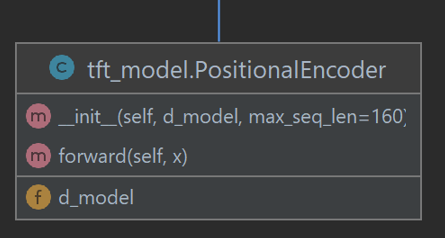
\includegraphics[scale = 0.8]{hd14}
    \caption{Positional Encoder}
\end{figure}
\subsubsection{Time Distributed}
\begin{figure}[H]
    \centering
    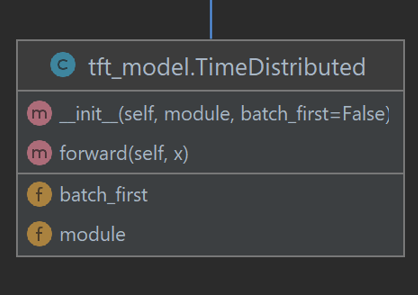
\includegraphics[scale = 0.8]{hd13}
    \caption{Time Distributed}
\end{figure}
\subsubsection{Activation Functions}
\begin{figure}[H]
    \centering
    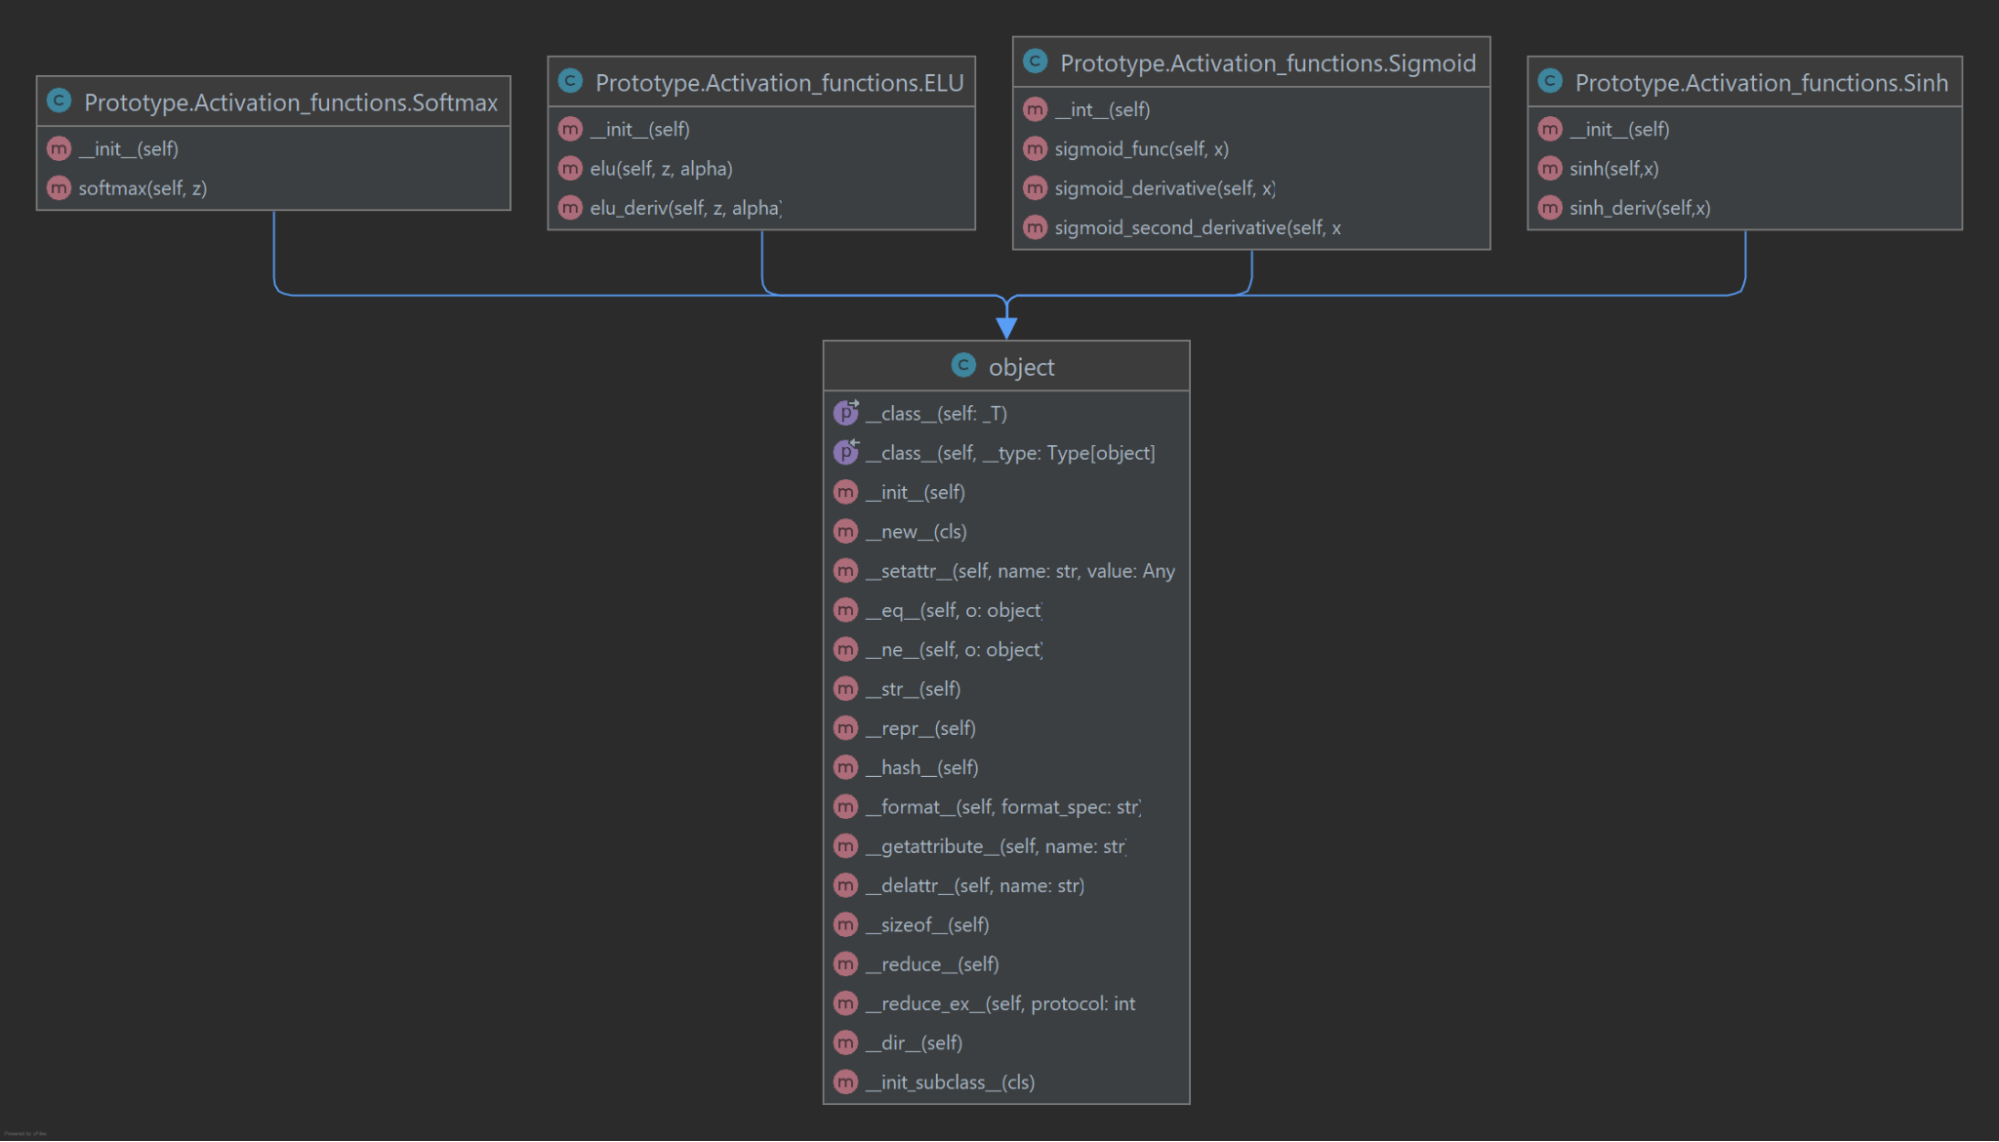
\includegraphics[scale = 0.2]{hd15}
    \caption{Activation Functions}
\end{figure}






\clearpage
\subsubsection{Model Layout}

The TFT can be modelled using the structure below. This shows the flow of data through one epoch of the network.  Each module has the dimensions, input features, output features, activation functions and learning rate specified.
These parameters are likely to be changed in the implementation but offer a great place to start as they are not too computationally intensive.
\\
Any Python code listed below in this section is used as part of my designing and prototyping.
\begin{lstlisting}
TemporalFusionTransformer(
  (loss): QuantileLoss()
  (logging_metrics): ModuleList(
    (0): SMAPE()
    (1): MAE()
    (2): RMSE()
    (3): MAPE()
  )
  (input_embeddings): MultiEmbedding(
    (embeddings): ModuleDict()
  )
  (prescalers): ModuleDict()
  (static_variable_selection): VariableSelectionNetwork(
    (single_variable_grns): ModuleDict()
    (prescalers): ModuleDict()
    (softmax): Softmax(dim=-1)
  )
  (encoder_variable_selection): VariableSelectionNetwork(
    (single_variable_grns): ModuleDict()
    (prescalers): ModuleDict()
    (softmax): Softmax(dim=-1)
  )
  (decoder_variable_selection): VariableSelectionNetwork(
    (single_variable_grns): ModuleDict()
    (prescalers): ModuleDict()
    (softmax): Softmax(dim=-1)
  )
  (static_context_variable_selection): GatedResidualNetwork(
    (fc1): Linear(in_features=16, out_features=16, bias=True)
    (elu): ELU(alpha=1.0)
    (fc2): Linear(in_features=16, out_features=16, bias=True)
    (gate_norm): GateAddNorm(
      (glu): GatedLinearUnit(
        (dropout): Dropout(p=0.1, inplace=False)
        (fc): Linear(in_features=16, out_features=32, bias=True)
      )
      (add_norm): AddNorm(
        (norm): LayerNorm((16,), eps=1e-05, elementwise_affine=True)
      )
    )
  )
  (static_context_initial_hidden_lstm): GatedResidualNetwork(
    (fc1): Linear(in_features=16, out_features=16, bias=True)
    (elu): ELU(alpha=1.0)
    (fc2): Linear(in_features=16, out_features=16, bias=True)
    (gate_norm): GateAddNorm(
      (glu): GatedLinearUnit(
        (dropout): Dropout(p=0.1, inplace=False)
        (fc): Linear(in_features=16, out_features=32, bias=True)
      )
      (add_norm): AddNorm(
        (norm): LayerNorm((16,), eps=1e-05, elementwise_affine=True)
      )
    )
  )
  (static_context_initial_cell_lstm): GatedResidualNetwork(
    (fc1): Linear(in_features=16, out_features=16, bias=True)
    (elu): ELU(alpha=1.0)
    (fc2): Linear(in_features=16, out_features=16, bias=True)
    (gate_norm): GateAddNorm(
      (glu): GatedLinearUnit(
        (dropout): Dropout(p=0.1, inplace=False)
        (fc): Linear(in_features=16, out_features=32, bias=True)
      )
      (add_norm): AddNorm(
        (norm): LayerNorm((16,), eps=1e-05, elementwise_affine=True)
      )
    )
  )
  (static_context_enrichment): GatedResidualNetwork(
    (fc1): Linear(in_features=16, out_features=16, bias=True)
    (elu): ELU(alpha=1.0)
    (fc2): Linear(in_features=16, out_features=16, bias=True)
    (gate_norm): GateAddNorm(
      (glu): GatedLinearUnit(
        (dropout): Dropout(p=0.1, inplace=False)
        (fc): Linear(in_features=16, out_features=32, bias=True)
      )
      (add_norm): AddNorm(
        (norm): LayerNorm((16,), eps=1e-05, elementwise_affine=True)
      )
    )
  )
  (lstm_encoder): LSTM(16, 16, batch_first=True)
  (lstm_decoder): LSTM(16, 16, batch_first=True)
  (post_lstm_gate_encoder): GatedLinearUnit(
    (dropout): Dropout(p=0.1, inplace=False)
    (fc): Linear(in_features=16, out_features=32, bias=True)
  )
  (post_lstm_gate_decoder): GatedLinearUnit(
    (dropout): Dropout(p=0.1, inplace=False)
    (fc): Linear(in_features=16, out_features=32, bias=True)
  )
  (post_lstm_add_norm_encoder): AddNorm(
    (norm): LayerNorm((16,), eps=1e-05, elementwise_affine=True)
  )
  (post_lstm_add_norm_decoder): AddNorm(
    (norm): LayerNorm((16,), eps=1e-05, elementwise_affine=True)
  )
  (static_enrichment): GatedResidualNetwork(
    (fc1): Linear(in_features=16, out_features=16, bias=True)
    (elu): ELU(alpha=1.0)
    (context): Linear(in_features=16, out_features=16, bias=False)
    (fc2): Linear(in_features=16, out_features=16, bias=True)
    (gate_norm): GateAddNorm(
      (glu): GatedLinearUnit(
        (dropout): Dropout(p=0.1, inplace=False)
        (fc): Linear(in_features=16, out_features=32, bias=True)
      )
      (add_norm): AddNorm(
        (norm): LayerNorm((16,), eps=1e-05, elementwise_affine=True)
      )
    )
  )
  (multihead_attn): InterpretableMultiHeadAttention(
    (dropout): Dropout(p=0.1, inplace=False)
    (v_layer): Linear(in_features=1, out_features=4, bias=True)
    (q_layers): ModuleList(
      (0): Linear(in_features=16, out_features=4, bias=True)
      (1): Linear(in_features=16, out_features=4, bias=True)
      (2): Linear(in_features=16, out_features=4, bias=True)
      (3): Linear(in_features=16, out_features=4, bias=True)
    )
    (k_layers): ModuleList(
      (0): Linear(in_features=16, out_features=4, bias=True)
      (1): Linear(in_features=16, out_features=4, bias=True)
      (2): Linear(in_features=16, out_features=4, bias=True)
      (3): Linear(in_features=16, out_features=4, bias=True)
    )
    (attention): ScaledDotProductAttention(
      (softmax): Softmax(dim=2)
    )
    (w_h): Linear(in_features=4, out_features=16, bias=False)
  )
  (post_attn_gate_norm): GateAddNorm(
    (glu): GatedLinearUnit(
      (dropout): Dropout(p=0.1, inplace=False)
      (fc): Linear(in_features=16, out_features=32, bias=True)
    )
    (add_norm): AddNorm(
      (norm): LayerNorm((16,), eps=1e-05, elementwise_affine=True)
    )
  )
  (pos_wise_ff): GatedResidualNetwork(
    (fc1): Linear(in_features=16, out_features=16, bias=True)
    (elu): ELU(alpha=1.0)
    (fc2): Linear(in_features=16, out_features=16, bias=True)
    (gate_norm): GateAddNorm(
      (glu): GatedLinearUnit(
        (dropout): Dropout(p=0.1, inplace=False)
        (fc): Linear(in_features=16, out_features=32, bias=True)
      )
      (add_norm): AddNorm(
        (norm): LayerNorm((16,), eps=1e-05, elementwise_affine=True)
      )
    )
  )
  (pre_output_gate_norm): GateAddNorm(
    (glu): GatedLinearUnit(
      (fc): Linear(in_features=16, out_features=32, bias=True)
    )
    (add_norm): AddNorm(
      (norm): LayerNorm((16,), eps=1e-05, elementwise_affine=True)
    )
  )
  (output_layer): Linear(in_features=16, out_features=7, bias=True)
)


\end{lstlisting}



\clearpage
\subsection{Explaining nn.module}
Below is the pseudocode for the module followed by the python code.
\begin{algorithm}
\caption{Linear Neural Network}
\begin{algorithmic}[1]
\For{Layer in network}
    \State {Convolution1 $\leftarrow$ ConvertTo2d(x,y,z)}
    \State {Convolution2 $\leftarrow$ ConvertTo2d(u,v,w)}
    \State {y $\leftarrow$ Wx + b}
    \State {fc1 $\leftarrow$ LinearTranformation()}
    \Comment{Apply a linear transformation}}
    \State {fc2 $\leftarrow$ LinearTranformation()}
    \State {fc3 $\leftarrow$ LinearTranformation()}
    \State {x $\leftarrow$ Apply2DPool(RELU(Convolution1(x)), (2, 2))}
    \State {x $\leftarrow$ Apply2DPool(RELU(Convolution1(x)),2 )}
    \State {RELU(fc1(x))}
    \State {RELU(fc2(x))}
    \State \Return{ $x$}
\EndFor{}
\end{algorithmic}
\end{algorithm}


\begin{lstlisting}
import math
import numpy as np

#Vanilla Neural Network from scratch
class Layer_Dense:
    def __init__(self, n_inputs, n_neurons):
        self.weights = 0.10 * np.random.randn(n_inputs, n_neurons)
        self.biases = np.zeros((1, n_neurons))

   def forward(self, inputs):
        self.output = np.dot(inputs, self.weights) + self.biases


#Activation Functions
class Activation_ReLU:
    def forward(self, inputs):
        self.output = np.maximum(0, inputs)

class Activation_sigmoid:
    def forward(self, inputs):
        self.output = np.exp()

layer1 = Layer_Dense(2,5)
activation1 = Activation_ReLU()
layer2 = Layer_Dense(2,5)
activation2 = Activation_sigmoid()
layer1.forward(X)
print(layer1.forward(x))


#using nn.module
class Net(nn.Module):

    def __init__(self):
        super(Net, self).__init__()
        # 1 input image channel, 6 output channels, 5x5 square convolution kernel
        self.conv1 = nn.Conv2d(1, 6, 5)
        self.conv2 = nn.Conv2d(6, 16, 5)

        # an affine operation: y = Wx + b
        self.fc1 = nn.Linear(16 * 5 * 5, 120)
        self.fc2 = nn.Linear(120, 84)
        self.fc3 = nn.Linear(84, 10)

    def forward(self, x):
        # Max pooling over a (2, 2) window
        x = F.max_pool2d(F.relu(self.conv1(x)), (2, 2))

        # 2 is ame as (2, 2)
        x = F.max_pool2d(F.relu(self.conv2(x)), 2)

        x = x.view(-1, self.num_flat_features(x))
        x = F.relu(self.fc1(x))
        x = F.relu(self.fc2(x))
        x = self.fc3(x)

        return x

    def num_flat_features(self, x):
        size = x.size()[1:]  # all dimensions except the batch dimension
        num_features = 1
        for s in size:       # Get the products
            num_features *= s
        return num_features
\end{lstlisting}

\clearpage

\subsection{Positional Encoding}
One of the reasons for using sine and cosine functions is that they are periodic and so whether the model is learning on a sequence of length 5, or of length 500, the encodings will always have the same range ([-1, 1]).  Positional embeddings are added to the original embeddings to retain all the positional information. Each vector will be parametrized and the stack row-wise to form a learnable positional embedding table.

%\begin{equation}
$PE_{pos+k}$ is some matrix which depends on k times  $PE_{pos}$
$$PE_{pos+k, 2i} = sin(\frac{pos}{a}+\frac{k}{a})$$
$$ =sin(\frac{pos}{a})cos(\frac{k}{a})+sin(\frac{k}{a})cos(\frac{pos}{a})$$
$$ =(PE_{pos,2i+1})U+(PE_{pos,2i})V$$
$$ =(PE_{pos,2i},PE_{pos,2i+1})(V,U)$$
%\end{equation}

\begin{algorithm}
\caption{Positional Encoder}
\begin{algorithmic}[1]
\For{pos in  0 $\leftarrow$ maximum sequence length}
    \State{compute V$\times$PE(pos,2i)}
    \State{compute W$\times$PE(pos,2i)}
    \State{compute V$\times$PE(pos,2i+1)}
    \State{compute W$\times$PE(pos,2i+1)}
\EndFor
\end{algorithmic}
\end{algorithm}


\\Python code:


\begin{lstlisting}
#positional encoding
import torch
import math


class PositionalEncoder(torch.nn.Module):
    def __init__(self, d_model, max_len=5000):
        self.d_model = d_model # the size of the embedding vectors
        self.max_len = max_len
        # Compute the positional encodings once in log space complexity
        pe = torch.zeros(max_len, d_model)
        position = torch.arange(0, max_len).unsqueeze(1)
        div_term = torch.exp(torch.arange(0, d_model, 2) *
                             -(math.log(10000.0) / d_model))
        pe[:, 0::2] = torch.sin(position * div_term)
        pe[:, 1::2] = torch.cos(position * div_term)
        pe = pe.unsqueeze(0)
        self.register_buffer('pe', pe)

    def forward(self, x):
        x = x + self.pe[:, :x.size(1)]
        return x

    def get_embedding(self, x):
        x = x + self.pe[:, :x.size(1)]
        return x

    def get_embedding_layer(self):
        return torch.nn.Embedding(self.max_len, self.d_model)

\end{lstlisting}
\clearpage
\subsection{Backpropagation}
The formula for the backpropagation algorithm has been proven earlier in the analysis. Below is a reminder of the mathematical definition along with a flowchart and pseudocode.

Partial derivatives:
$$\frac{\partial{E_d}}{\partial{w_j^k}} = \delta_j^k o_i^{k-1}$$
Final layer's error term:
$$\delta_1^m = g_o'(a_1^m)(\hat{y_d-y_d})$$
Hidden layers' error terms:
$$\delta_j^k = g''(a_j^k)\sum_{L=1}^{r^{k+1}}w^{k+1}_jL\delta_l^{k+1}$$
Computing the partial derivatives for each input-output pair:
    $$\frac{\partial{E(X,\theta)}}{\partial{w_ij^k}}= \frac{1}{N}\sum_{d=1}^{N}\frac{\delta}{\delta w_ij^k}(\frac{1}{2}(\hat{y_d}-y_d)^2)$$
    $$ = \frac{1}{N}\sum_{d=1}^{N}\frac{\partial{E_d}}{\partial{w_ij^k}}$$
Updating weights:
$$ \Delta w_ij^k = -\alpha \frac{\partial{E(X,\theta)}}{\partial{w_ij^k}}$$
\begin{algorithm}
\caption{Backpropagation}
\begin{algorithmic}[1]
\Function{Backpropagation}{inputs, expected, output}
    \State {deltas $\leftarrow$delta inputs}
    \Repeat{ Layers}
    \For{i in deltas}
        \State{error $\leftarrow$ expected[i] - output
        deltas[i]$\leftarrow$ error$\times$sigmoid}
    \For{j in hidden layers}
        \For{k in hidden weights}
           \State{delta weights$\leftarrow$ weight[j] $\times$ outputdeltas[k]}
            \State{deltaweights$\times$ learning rate}
            \EndFor
            \EndFor
\EndFunction
\end{algorithmic}
\end{algorithm}
\clearpage
\begin{lstlisting}
# backpropagate() takes as input, the patterns entered, the target values and the obtained values.
# Based on these values, it adjusts the weights so as to balance out the error.
# Also, now we have M, N for momentum and learning factors respectively.
def backpropagate(self, inputs, expected, output, N=0.5, M=0.1):
	# We introduce a new matrix called the deltas (error) for the two layers output and hidden layer respectively.
	output_deltas = [0.0]*self.no
	for k in range(self.no):
		# Error is equal to (Target value - Output value)
		error = expected[k] - output[k]
		output_deltas[k]=error*dsigmoid(self.ao[k])

	# Change weights of hidden to output layer accordingly.
	for j in range(self.nh):
		for k in range(self.no):
			delta_weight = self.ah[j] * output_deltas[k]
			self.who[j][k]+= M*self.cho[j][k] + N*delta_weight
			self.cho[j][k]=delta_weight

	# Now for the hidden layer.
	hidden_deltas = [0.0]*self.nh
	for j in range(self.nh):
		# Error as given by formule is equal to the sum of (Weight from each node in hidden layer times output delta of output node)
		# Hence delta for hidden layer = sum (self.who[j][k]*output_deltas[k])
		error=0.0
		for k in range(self.no):
			error+=self.who[j][k] * output_deltas[k]
		# now, change in node weight is given by dsigmoid() of activation of each hidden node times the error.
		hidden_deltas[j]= error * dsigmoid(self.ah[j])

	for i in range(self.ni):
		for j in range(self.nh):
			delta_weight = hidden_deltas[j] * self.ai[i]
			self.wih[i][j]+= M*self.cih[i][j] + N*delta_weight
			self.cih[i][j]=delta_weight
\end{lstlisting}
\clearpage
\subsection{Dense Network}
This is the fundamental block, similar to the nn.module. This is another vanilla
neural network.

\begin{lstlisting}
class Dense_Network:
    def __init__(self, input_shape, output_shape, activation, weights, biases):
        self.input_shape = input_shape
        self.output_shape = output_shape
        self.activation = activation
        self.weights = weights
        self.biases = biases
        self.output = None
        self.input = None

    def forward_pass(self, input):
        self.input = input
        self.output = np.dot(self.input, self.weights) + self.biases
        self.output = self.activation(self.output)
        return self.output

    def backward_pass(self, error):
        self.error = error
        self.error = self.error * self.activation(self.output, derivative=True)
        self.weights_error = np.dot(self.input.T, self.error)
        self.biases_error = np.sum(self.error, axis=0)
        return self.error

    def update_weights(self, learning_rate):
        self.weights = self.weights - learning_rate * self.weights_error
        self.biases = self.biases - learning_rate * self.biases_error

    def get_weights(self):
        return self.weights


\end{lstlisting}

\clearpage


\subsection{Weight Initialisation}
\subsubsection{Theory}
Weight initialisation is essential when training a neural network. This process prevents
activation functions from exploding or vanishing when executing a forward pass. If the weights are too large, the variance of the input data tends to increase rapidly with each pass, eventually
getting to a point where the derivative tends to 0. This is why it is important to initialise the network with the right weights. The range in which the it is initialised will be governed using a technique called Xavier initialisation.\\
Xavier works by assigning the weights from a Gaussian distribution
Consider a distribution with mean 0 and some finite variance as well as a linear neuron: $$y = w_1x_1 + w_2x_2 + ... + b$$
With each forward pass we would like the variance to remain the same.
Let's first compute the variance of y:
$$var(y) = var(w_1x_1 + w_2x_2 + ...+w_nx_n + b)$$
Let's computer the variance of the terms inside the brackets as well. Considering the general term would give us:
$$var(w_ix_i) = E(x_i)^2var(w_i) + E(w_i)^2var(x_i) + var(w_i)var(x_i)$$
Where E() represents the expectation of a given variable. The assumption that the inputs and weights are generated from a Gaussian distrubtion with a mean 0 allows us to ignore the
expectation, giving us:
$$var(w_ix_i) = var(w_i)var(x_i) $$
Substituting this value back into our original equation gives us:
$$var(y) = var(w_1)var(x_1)+ ... + var(w_n)var(x_n)$$
As these are distributed identically, they can be written as:
$$var(y) = N \times var(w_i) \times var(x_i)$$
If we want the variance of y to be the same as x, we should set $N\times var(w_i) = 1$, giving us:
$var(w_i) = \frac{1}{N}$
\\This leaves us with the final formula:
$$var(w_i) = \frac{1}{N_{avg}}$$
where $$N_{avg} = \frac{(N_{in} + N_{out})}{2}$$
The average helps preserve the backpropagated signal but is more computationally complex to implement.



\begin{algorithm}
\caption{Using Xaviar}
\begin{algorithmic}[1]
\State{Initialise weights using Xavier}
\While{not Stop-Criterion}
    \For{all i, j}
    \State{$w_{i,j}$ = $w_{i,j}$ - $\alpha$*$\frac{\partial{Error}}{\partial{w_{i,j}}}$}
    \EndFor{}
\EndWhile{}
\end{algorithmic}
\end{algorithm}

\subsection{Layer Normalisation}

\subsubsection{The need for normalisation}
The main issue that normalisation works to solve is the problem of internal
covariate shift. These shifts occur during each epoch/round of training due to weights
being updated and different data being processed. This means that each input to a
neuron is slightly different each time. The input distribution of the inputs starts
to deform.
These small changes would have an insignificant impact on smaller architectures
such as a single lstm or a vanilla RNN but when dealing with bigger models such as Transformers
or TFTs small changes in the input distribution can amplify and have a catastrophic
impact on the deep learning.
Normalisation also tackles the vanishing gradient issue. This is where the activation
function saturates. The functions approach a limit as the inputs tend to large values.
This limit is where the gradient starts to shrink to a point where the function becomes
unusable. As discussed in the activation functions section, different activation functions
can be used to mitigate this problem as well as normalising the inputs.

\subsubsection{Layer Normalisation}


Given inputs $x$ over a batch size $m$, $B = {x_1,x_2, ..., x_m}$, each sample $x_i$ contains $K$ elements by applying transformations of the inputs using learned parameters
$\gamma$ and $\beta$, the outputs could be expressed as $B' = {y_1,y_2,...,y_m}$ where
$y_i=LN_{\gamma,\beta}(x_i)$. \\
We first start of by calculating the mean and variance of each sample from the batch.
For sample $x$, we have the mean, $\mu_i$, and the variance, $\sigma_i^2$
$$\mu_i = \frac{1}{K}\sum^K_{k=1}x_{i,k}$$
$$\sigma_i^2 = \frac{1}{K}\sum^K_{k=1}(x_{i,k}-\mu_i)^2$$
Each sample is then normalised around a zero mean and unit variance. $\epsilon$ has been used for numerical stability in case the denominator becomes zero.
$$\hat{x_i},k= \frac{x_{i,k}-\mu_i}{\sqrt{\sigma_i^2+\epsilon}}$$
Scaling and shifting is then finally done using $\gamma$ and $\beta$ which are learnable parameters.
$$ey_i = \gamma \hat{x_i}+\beta \equiv LN_{\gamma,\beta}(x_i)$$
The maths above shows how this normalisation technique has no dependancy on other samples in the batch.
\subsubsection{Batch normalisation vs layer normalisation}
Batch normalisation has a few issues that are key to training a TFT. One of which is that
it is hard to parallelise batch-normalised models. The dependancy between all the elements
 means that there is a need for synchronisation across all devices being used to train the model. Transformer models such as a TFT require a large scale setup to combat the
 mathematical complexity and intensities. Layer normalisation provides some degree of
 normalisation while not needing a dependancy on other elements making it more suitable
 for my model.
\subsubsection{Code}
\begin{lstlisting}
def ln(input, s, b, epsilon = 1e-5, max = 1000):
    """ Layer normalizes a 2D tensor along its second axis, which corresponds to batch """
    m, v = tf.nn.moments(input, [1], keep_dims=True)
    normalised_input = (input - m) / tf.sqrt(v + epsilon)
    return normalised_input * s + b
\end{lstlisting}
\clearpage





\subsection{Time Distributed}
Time Distributed

\begin{lstlisting}
class TimeDistributed(nn.Module):
    def __init__(self, module, batch_first=False):
        super(TimeDistributed, self).__init__()
        self.module = module
        self.batch_first = batch_first

    def forward(self, x):
        if len(x.size()) <= 2:
            return self.module(x)
        # Squash samples and timesteps into a single axis
        x_reshape = x.contiguous().view(-1, x.size(-1))  # (samples * timesteps, input_size)
        y = self.module(x_reshape)
        # We have to reshape Y
        if self.batch_first:
            y = y.contiguous().view(x.size(0), -1, y.size(-1))  # (samples, timesteps, output_size)
        else:
            y = y.view(-1, x.size(1), y.size(-1))  # (timesteps, samples, output_size)

        return y
\end{lstlisting}


\subsection{Activation Functions}
The use of activation functions has been explained in the analysis. This section
aims to provide a further understanding of how the functions are being coded and
optimisation techniques I have uncovered in the process.
\subsubsection{Sigmoid}
\begin{lstlisting}
class Sigmoid:
    def __int__(self):
        super().__init__()

    def sigmoid_func(self, x):
        return 1 / (1 + np.exp(-x))  # Calculates the sigmoid r

    def sigmoid_derivative(self, x):
        func_x = self.sigmoid_func(x)

        return func_x * (1 - func_x)

    def sigmoid_second_derivative(self, x):
        fn_x = self.fn(x)
        return fn_x * (1 - fn_x) * (1 - 2 * fn_x)

\end{lstlisting}
\subsubsection{Softmax}
The softmax function


\begin{lstlisting}
class Softmax():
    def __int__(self):
        super().__init__()

    def softmax(self, z):
        assert len(z.shape) == 2
        s = np.max(z, axis=1)
        s = s[:, np.newaxis]  # necessary step to do broadcasting
        e_x = np.exp(z - s)
        div = np.sum(e_x, axis=1)
        div = div[:, np.newaxis] # dito
        return e_x / div
\end{lstlisting}


\subsubsection{Tanh}
Here I am able to use the sinh definition to generate the first and second
derivatives. I can also use these definitions to form the tanh function.


\begin{lstlisting}
class Sinh:
    def __init__(self):
        super().__init__()

    def sinh(self,x):
        #doublesinh = np.exp(x) – np.exp(-x)
        comp1 = np.exp(x)
        comp2 = np.exp(-x)
        comp3 = 0.5 * (comp1-comp2)
        return comp3

    def sinh_deriv(self,x):
        # doublesinh = np.exp(x) – np.exp(-x)
        comp1 = np.exp(x)
        comp2 = np.exp(-x)
        final = 0.5 * (comp1 + comp2)
        return final

x = Sinh()
const = 1
tanh = (x.sinh(const))/(x.sinh_deriv(const))
\end{lstlisting}


\subsubsection{ELU}
\begin{lstlisting}
class ELU:
    def __init__(self):
        super().__init__()

    def elu(self, z, alpha):
        return z if z >= 0 else alpha * (np.exp(z) - 1)

    def elu_deriv(self, z, alpha):
        return 1 if z > 0 else alpha * np.exp(z)
\end{lstlisting}


\subsection{Attention}
\subsubsection{Multi-head attention}
Multihead attention is done by passing the output tensord through a series of functions.
The first step is to split the tensor into its neurons. The query and key is multiplied.
A mask is then used before it is passed through the softmax function. Though, as
previously discussed, the softmax is a very inefficient function, I have not been
able to source a more efficient algorithm that also produced probabilistic outputs.
The query vector is the masked before it is multiplied to the attention vector.
This is then split and normalised before returned back to the network.
Multihead attention is a parallel task with all heads running at the same time. Bigger
models may require 8-12 heads but for my data, 4 should be appropriate for me. This
is because multihead attention is a polynomial space complex algorithm so each head
will increase the memory needed polynomially. With the hardware I am operating with,
4 will push the system but not cause problems. Larger number of heads are required when
dealing with natural language processing. The nature of my data, time series data, means I can get away with a smaller number of heads.


\begin{algorithm}
    \caption{Attention}
    \begin{algorithmic}[1]
        \For{Indexed item in network}
    \State{x = Sqrt(key)}
    \State  \Return{ softmax(num / denum) $\cdot$ V}
    \EndFor{}
    \end{algorithmic}
\end{algorithm}
\clearpage
Below is the MultiHead attention algorithm

\begin{algorithm}
    \caption{MultiHead Attention}
    \begin{algorithmic}[1]
    \For {head in heads}
        \For{Indexed item in network}
            \State x = Sqrt(key)
            \State head_i =  softmax(num / denum) $\cdot$ V
        \EndFor{}
       \State $Concat(head_{i-1},head_i)$
    \EndFor{}
    \State \Return{Query $\times$ Concat(head_0 ... , head_i)}

    \end{algorithmic}
\end{algorithm}
Python Testing Code:
\begin{lstlisting}
    def MultiHeadAttention(self,
                Q, K, V):
        num_heads = self.num_heads
        N = Q.size()[0]
        # Linear projections
        Q_l = nn.ReLU()(self.linear_Q(Q))
        K_l = nn.ReLU()(self.linear_K(K))
        V_l = nn.ReLU()(self.linear_V(V))
        # Split and concat
        Q_split = Q_l.split(split_size=self.hidden_dim // num_heads, dim=2)
        K_split = K_l.split(split_size=self.hidden_dim // num_heads, dim=2)
        V_split = V_l.split(split_size=self.hidden_dim // num_heads, dim=2)
        Q_ = torch.cat(Q_split, dim=0)  # (h*N, T_q, C/h)
        K_ = torch.cat(K_split, dim=0)  # (h*N, T_k, C/h)
        V_ = torch.cat(V_split, dim=0)  # (h*N, T_v, C/h)
        # Multiplication
        outputs = torch.bmm(Q_, K_.transpose(2, 1))
        # Scale
        outputs = outputs / (K_.size()[-1] ** 0.5)
        # Key Masking
        key_masks = torch.sign(torch.abs(K).sum(dim=-1))  # (N, T_k)
        key_masks = key_masks.repeat(num_heads, 1)  # (h*N, T_k)
        key_masks = key_masks.unsqueeze(1).repeat(1, Q.size()[1], 1)  # (h*N, T_q, T_k)
        paddings = torch.ones_like(key_masks) * (-2 ** 32 + 1)
        outputs = torch.where(torch.eq(key_masks, 0), paddings, outputs)  # (h*N, T_q, T_k)
        # Activation
        outputs = nn.Softmax(dim=2)(outputs)  # (h*N, T_q, T_k)
        # Query Masking
        query_masks = torch.sign(torch.abs(Q).sum(dim=-1))  # (N, T_q)
        query_masks = query_masks.repeat(num_heads, 1)  # (h*N, T_q)
        query_masks = query_masks.unsqueeze(-1).repeat(1, 1, K.size()[1])  # (h*N, T_q, T_k)
        outputs = outputs * query_masks  # broadcasting. (h*N, T_q, T_k)
        # Dropouts
        outputs = self.dropout(outputs)
        # Weighted sum
        outputs = torch.bmm(outputs, V_)  # ( h*N, T_q, C/h)
        # Restore shape
        outputs = outputs.split(N, dim=0)  # (N, T_q, C)
        outputs = torch.cat(outputs, dim=2)
        # Residual connection
        outputs = outputs + Q_l
        # Normalize
        outputs = self.norm(outputs)  # (N, T_q, C)
        return outputs

\end{lstlisting}
\clearpage

\subsection{Loss Functions}

\subsubsection{Quantile Loss}
The loss function I have opted to go for is quantile loss. This produces outputs
at different quantiles. This function is useful when dealing with uncertainties.
Specifically for my project, I want to indicate to the user what the lower and
upper boundaries might be to give an indication of performance of the stock.

Given a prediction $y_p$ and outcome $y_i$, the regression loss for a quantile
loss $q$ is:
$$QuantileLoss(y_p,y_i) = max[q(y_i -y_p),(q-1)(y_i - y_p)]$$

Quantile of a random variable:

Let $Y$ be a real valued random variable with cumulative distribution function
$ F_Y(y) = P(Y<y)=$. The $\tau$th quantile of $Y$ is given by:
$$q_Y(\tau) = F^{-1}_Y(\tau) = inf(y:F_y(Y)\geq \tau ) $$
The loss function can be defined as $$\rho_{\tau}(y) = y(\tau - \mathbb{I})$$
A specific quantile can be found by minimising the expected loss of $Y$ with
respect to u:
$$q_Y(\tau) arg min E(\rho_{\tau}(Y - u)) = arg min {(\tau -1) \int _{\infty \:}^{\:u}\left(y-u\right)dF_Y\left(y\right)+\tau \int _{\infty \:}^{\:u}\left(y-u\right)dF_Y\left(y\right)+\tau } $$


This can also be shown by computing the derivative of the expected loss via
the Leibniz integral rule, setting it to 0 and letting $q_{\tau}$ be the solution
of

$$0 = \left(1-\tau \right)\int _{-\infty }^{q_{\tau }}dF_Y\left(y\right)\:-\:\tau \int _{q_{\tau }}^{\infty \:}dF_Y\left(y\right)\:\: $$

This then can be reduced to:
$$F_Yq(q_{\tau}) = \tau$$

This function has asymptotic properties. When $\tau$ is 0 or 1, the calculation
is slightly different but can be ignored for the context I am working within.


\begin{algorithm}
    \caption{Quantile Loss}
    \begin{algorithmic}[1]
    \For{i, quantile in quantiles}
        \State error = target - prediction
        \State x = (q-1)$\times$errors$\times$
        \State y = q$\times$errors
        \State loss = max(x,y)
    \EndFor
    \State \Return loss

    \end{algorithmic}
\end{algorithm}




\clearpage


\subsubsection{Poisson Loss}
Note that the Poisson loss is not actively used but is a useful function to know
of in this area of machine learning/statistical learning. \\
The model assumes that the variable Y has a Poisson distrubtion and that the log
of its expected value can be modelled by a linear combination of unknown
parameters.\\
The Poisson distribution is defined as: $$\frac{\lambda^y e^{-\lambda}}{y!}$$
This makes the probability mass function to be defined as:
$$\frac{e^{y\theta'x}e^{-e^{\theta'x}}}{y!}$$
By the method of maximum likelihood, we can find a set of parameters that maximises
the function. To do that the equation must first be written in terms of $\theta$ for a particular set of data:
$$\prod _{i=1}^{m}\frac{e^{y_i\theta'x_i}e^{-e^{\theta'x_i}}}{y_i!}$$

To make the equation easier to manipulate, it can be written as:
$$\sum_{i=1}^m (y_i\theta'x_i - e^{\theta'x_i} - log(y_i!))$$

Theta only appears in the first 2 terms so the $y!$ can be ignored to give just:
$$\sum_{i=1}^m (y_i\theta'x_i - e^{\theta'x_i})$$

To find a maximum, the differential must be taken and set to 0. This equation
unfortunately does not have any solutions as the functions is convex. This is where
techniques such as gradient descent must be applied to find an optimal value for
$\theta$. This algorithm is described earlier in the paper.

\clearpage
\subsection{Data Structures}
The data is initially stored in a CSV file. The data is then converted into a 2x1 matrix before it is turned into a 2x2 matrix. These are implemented using lists in python. The data, as it goes through the model, gets converted into tensors.
The attention module is modelled using dictionaries.
My weights will also be stored in tensors.
Derivatives will be stored in a Jacobian matrix.
\clearpage








\subsection{File Structure}
Data
\begin{itemize}
\item Training
\item Stock data
\item Validation
\item Pre-training alternate dataset
\end{itemize}
Modules
\begin{itemize}
\item Data Pre-processing
\item Activation Functions
\item Attention module
\item Data loaders
\item Dense Network
\item Gated Linear Unit
\item Layer Normalisation
\item LSTM
\item Positional Encoder
\item Time Distributed layer
\item Variable Selection Network
\item Loss Functions
\item Batch Normalisation
\item OZE Loss
\item Dense Block
\item MutiHead Attention
\item Main TFT
\item Quantile Forecasts
\item Model Tuning
\end{itemize}






\section{Coding Process}

After setting up a smaller TFT on a reduced dataset, errors started to reveal
themselves. One big issue was dying neurons. Using a biological metaphor,
it can be described as brain damage. This issue may be caused by having a
model that is too big for the data or could be as intricate as vanishing gradient
occurring in the activation functions.\\
I am runnning a learning rate of 0.0005, this is based of a hyper parameter
estimation algorithm provided by pytorch. I have a hidden size of 128 but this
may change later on to gain a higher accuracy. The attention head size is 2 with
a dropout of 0.1. I am using quantile loss on the model. The prediction length
is 5 as I do not have enough ram to accommodate more. I also aimed to run
the program for 150 epochs/loops with each epoch taking roughly 11 minutes.
I have faced issues with being dimensionally consistent throughout my code.
Some tensors have been bigger than others which create errors when performing
complex matrix operations. This was solved by reshaping the tensor using
pytorch’s tools.\\
There were also problems related to the encoder and decoder lengths. This was
resolved by looking at the data and working out what input size gave the most
reliable results. This meant that the program is now specific to the dataset and
lots of variables would have to be tweaked to accommodate a different dataset.
I was also having errors with converting lists into tensors that allow only floats
and Tensors that only allow doubles. Lots of functions created tensors that were
doubles and would not be accepted by the next block as they were the wrong
type.\\
Attribute errors were also common where I had called on functions that had
not been inherited properly. This only became clear near the end of the project
when I was assembling the model. This was because data was not being passed
through the forward pass function properly.\\
Assertion errors were quite common where I had asserted statements that did
not follow the logic.\\
Index errors were common where I was trying to access data in Tensors. This
was resolved quickly once I started using the Pytorch tensors.\\
IsADirectoryErrors cropped up quite a bit due to accessing parts of the model
that were not present. I also came across this issue when trying to access the
saved model.\\
Saving and loading the model was a big problem that I decided not to spend
more time on. This means that the user will have to load the dataset they wish
to use and then run the model to gain access to the predictions.\\
Understanding the dataset and what model size should be applied to it proved
to be more difficult than initially existed. The parameters that were finally used
came about using trial and error. This is shown in my parameter testing. There
might be better ways to go about it but I did not pursue them.\\
I was not able to get all the modules to flow into each other by scratch but
the model did work when I assembled it using Pytorch. This will be further
explained in the Evaluation section.\\
The plan was to originally to store the data in a database but this proved to be
inefficient and a waste of my client's resources. CSV files were more appropriate
for this use case. The code for the database is present as well as the database itself.
This will be listed in DBtoPY.\\
Initially I had considered using OZE loss but this later turned into Quantile loss
once I realised the benefits.
\subsection{Autograd}
To differentiate Tensors I had to use tools such as Autograd. This is because
partial differentiation of tensors proved to be harder than anticipated. Writing
a module to do this would have taken a lot of time and would be hugely inefficient.
Autograd is an automatic differentiation package that is used on floating point
tensors.
\clearpage
\section{Modular Testing}


\subsection{Parameter Testing}

\begin{figure}[H]
    \centering
    \includegraphics[scale=0.6]{Tests/ParamTest}
\end{figure}

\begin{figure}[H]
    \centering
    \includegraphics[scale=0.6]{Tests/ParamTest2}
\end{figure}

\subsubsection{Issues}
Trying to find the best parameters proved to be more difficult than anticipated.
Testing each parameter took roughly 10 minutes and sometimes the program crashed
due to needing more resources than needed.

\subsection{GRN.py}

\begin{figure}[H]
    \centering
    \includegraphics[scale=0.4]{Tests/GRN1}
\end{figure}

\begin{figure}[H]
    \centering
    \includegraphics[scale=0.4]{Tests/GRN2}
\end{figure}

\subsubsection{Issues}
Trying to feed a layer forward was the most difficult part. I also had to use
the temporal layer class so that I could implement attention. This was also
quite difficult. This was where I had to research the
np.shape() function. Attribute errors were also common.

\subsection{ActivationFunctions.py}

\begin{figure}[H]
    \centering
    \includegraphics[scale=0.6]{Tests/AF1}
\end{figure}

\begin{figure}[H]
    \centering
    \includegraphics[scale=0.6]{Tests/AF2}
\end{figure}

\begin{figure}[H]
    \centering
    \includegraphics[scale=0.6]{Tests/AF3}
\end{figure}

\subsubsection{Issues}
There weren't many issues encountered as this file focussed on defining
mathematical objects using numpy. The hardest part was setting out the acceptance
and rejection states. I also had to make sure I was using the right type of tensors,
Pytorch tensors instead of numpy tensors. This was related to passing layers through.

\subsection{LossFunctions.py}

\begin{figure}[H]
    \centering
    \includegraphics[scale=0.6]{Tests/Loss}
\end{figure}

\subsubsection{Issues}
The hardest part here was extracting the values and performing the
calculations in the forward() function. This is where I was introduced to the axis
parameter that could be change. This is where I was introduced to the axis
parameter that could be changed to access the columns that were required.

\subsection{GLU.py}

\begin{figure}[H]
    \centering
    \includegraphics[scale=0.6]{Tests/GLU1}
\end{figure}


\begin{figure}[H]
    \centering
    \includegraphics[scale=0.6]{Tests/GLU2}
\end{figure}

\subsubsection{Issues}
I didn't encounter many problems here as all that was required was a multiplication
between matrices with the use the Sigmoid activation function.
\subsection{DenseNetwork.py}

\begin{figure}[H]
    \centering
    \includegraphics[scale=0.75]{Tests/Dense1}
\end{figure}

\begin{figure}[H]
    \centering
    \includegraphics[scale=0.75]{Tests/Dense2}
\end{figure}
\subsubsection{Issues}
This was a relatively simple function where there was a standard initialisation
with a few parameters. The forward and back pass was straightforward as I was
just using the partial derivatives to compute the pass. This process has been
explained in the documented design.

\subsection{PositionalEncoder.py}
\begin{figure}[H]
    \centering
    \includegraphics[scale=0.8]{Tests/PE1}
\end{figure}
\begin{figure}[H]
    \centering
    \includegraphics[scale=0.8]{Tests/PE2}
\end{figure}
Below is the testing video:\\
https://youtu.be/Hb3bgGF47Do
\begin{figure}[H]
    \centering
    \includegraphics[scale=0.5]{Tests/QR4}
\end{figure}

\subsubsection{Issues}
The main issue here was understanding how the trignometric functions accepted
the data as an input.
\subsection{DataPreprocessing.py}

\begin{figure}[H]
    \centering
    \includegraphics[scale=0.6]{Tests/DP}
\end{figure}

\clearpage
\subsubsection{Issues}
This was an easier section where classes allowed for a neater solution. The biggest
issue here was the batch normalisation that required time to fully understand.

\subsection{PytorchForecasting.py}
\begin{figure}[H]
    \centering
    \includegraphics[scale=0.7]{Tests/PF1}
\end{figure}
\begin{figure}[H]
    \centering
    \includegraphics[scale=0.7]{Tests/PF2}
\end{figure}
Below is the testing video:
\\https://youtu.be/AM0zitft430
\begin{figure}[H]
    \centering
    \includegraphics[scale=0.5]{Tests/QR3}
\end{figure}
\subsubsection{Issues}
This module had me assemble the Pytorch model. The biggest challenge was understanding
how the encoder and decoder lengths worked. This is not well documented online
so research papers were required to try and understand it. This was eventually fixed
after I tested the parameter and monitored its behaviour.
\subsection{AttentionModule.py}

\begin{figure}[H]
    \centering
    \includegraphics[scale=0.7]{Tests/MH1}
\end{figure}
\begin{figure}[H]
    \centering
    \includegraphics[scale=0.7]{Tests/MH2}
\end{figure}
\subsubsection{Issues}
This module has been the most challenging to code. The actual formula and process
is well documented and designed but I was experiencing a lot of problems with
type of input. This module takes tensors as an input and then works out a score
for all the values based off a key, value and query. I was able to implement the
query, value and key calculations as well as combining scores when conducting
multihead attention. I was unfortunately not able to process the Tensor layers
manually but instead had to rely on Pytorch's tools to do it. I was getting
type errors that were very ambiguous and not easy to solve. Passing a tensor
straight into the function did resolve the problem which indicates there is
a more subtle issue in the code. This meant individually all the functions worked.

\subsection{LSTM.py}
\begin{figure}[H]
    \centering
    \includegraphics[scale=0.7]{Tests/LSTM1}
\end{figure}
Below is the testing video:
\\https://youtu.be/G5fJAKKu7QM
\begin{figure}[H]
    \centering
    \includegraphics[scale=0.5]{Tests/QR5}
\end{figure}
\subsubsection{Issues}
This section was relatively straight forward as I just had to set up initial
weights and biases before backpropagating through them. The flow chart listed in
the documented design made it easy to code in. The hardest part getting it to
work seamlessly with other functions. As with most of this project, the biggest
difficulty was allowing data to flow freely between all the modules, something I
was not able to do.

\subsection{Main.py}
Testing this module proved to be quite challenging as this could only work with
the actual dataset rather than artificial tensors.
\\
This function does not work correctly as I have an issue with the Variable Selection Network.
All the other modules do get initiated which shows that the rest of the modules get assembled.
This means this module can still pass the test if considered independently.
\\This file also runs the Pytorch version of the model as that is the model that
is being used to train the model.
\clearpage
\section{System Testing}

The whole system was tested using different parameters. The first QR code is a
video of a reduced system running with a hidden size of 4, encoder size of 2000
and a learning rate of 0.05.\\
The second QR code is a video of the same reduced system but with a hidden
size of 2.
\\https://youtu.be/fLJoFLTra78
\begin{figure}[H]
    \centering
    \includegraphics[scale=0.6]{Tests/QR1}
\end{figure}
The videos also demonstrate the difference the parameters make to the qual-
ity of the predictions. The graphs will be explained in the Results section.
\\https://youtu.be/jWCOhgnw-Vw
\begin{figure}[H]
    \centering
    \includegraphics[scale=0.6]{Tests/QR2}
\end{figure}

\clearpage

\section{Objective Testing}

\begin{figure}[H]
    \centering
    \includegraphics[scale=0.7]{Tests/O1}
\end{figure}
\begin{figure}[H]
    \centering
    \includegraphics[scale=0.7]{Tests/O2}
\end{figure}
\begin{figure}[H]
    \centering
    \includegraphics[scale=0.7]{Tests/O3}
\end{figure}
\begin{figure}[H]
    \centering
    \includegraphics[scale=0.7]{Tests/O4}
\end{figure}
\begin{figure}[H]
    \centering
    \includegraphics[scale=0.7]{Tests/O5}
\end{figure}
I was able to meet nearly all of my objectives. The only failed test was the
Variable Selection Network. This was expected and I didn't anticipate the model
that was built from scratch to work with 100\% accuracy. This could've been achieved
has I chosen a smaller, easier model but those did not have the technologies
such as attention that are utilised in this model. My model with pytorch
works flawlessly so I am still able to provide my client with a working stock
trend indicator as was expected. This means I do satisfy all the objectives.
\clearpage

\section{Results}

Below are a series of images from running the code several times. Each image
will be complemented with a bit of commentary. In each of the figures, the blue
line indicates what the actual price was and the orange line is what my model
has predicted. A few general comments can be made beforehand, in each of the
tests it is clear that the model to smooth the graphs indicating that it did not
deal with volatility very well. This makes the model better suited for long term
trends rather than short term volatility. This limits the trading strategies this
can be used in but is better for amateur/casual investors who are more focussed
on simple strategies that include a stock price going up or down. This model is
better suited for commodities and ETFs rather than stocks. This model should
not be used to predict prices of crypto currencies or such tradeable assets that
will have instantaneous spikes. In most of the tests below, I have run a reduced
model with very low epoch runs. This has a huge impact on the quality of the
outputs.\\
Some graphs may have shaded orange sections. These are the quantiles and
can be used to give the user an estimate of the potential highs and lows in that
prediction. This may influence the trading strategy that they might employ.
\\
All tests listed below were run on a device with the following specification:\\
i7-8550u\\
8gb RAM \\
Intel UHD 620 integrated graphics \\
Manjaro Linux\\
\\
When running the program on the same device but in Windows, the results were very
different. Average training time was up by 460\%. Average loss was also up by
50\% which indicates a problem in resource management in Windows. Because of this,
I would recommend running the code on a Linux machine. I was not able to run the
code on Mac OS to verify if it was an optimisation issue or just an issue with
Windows.


\clearpage


\subsection{Test 1}
\begin{figure}[H]
    \centering
    \includegraphics[scale=0.4]{Tests/r1}
    \caption{}
\end{figure}
Here you can see that the model has identified the lows in the graph and was
heavily influenced in them at the start resulting in a low curve. This then
gradually increases predicting an eventual increase in the stock price over the
next few days. This is not exactly what happens in the actual price but does
loosely follow the trend that was predicted.
\begin{figure}[H]
    \centering
    \includegraphics[scale=0.25]{Tests/r2}
    \caption{}
\end{figure}
These are the high averages for the FTSE price. These follow a similar trend
to the close averages above. This is what we would expect. It was able to predict
the price with very high accuracy on the last point which is reassuring.

\subsection{Test 2}
\begin{figure}[H]
    \centering
    \includegraphics[scale=0.25]{Tests/r3}
    \caption{}
\end{figure}
Here is an example where there is severe overfitting. This has resulted in the
neurons dying/ not being activated in the later epochs. This results in the
network assuming a value and then sticking to it. This issue can be resolved by
increasing the size of the dataset, reducing the size of the network or changing
the activation function. Using a RELU can result in the vanishing gradient
problem occurring.
\begin{figure}[H]
    \centering
    \includegraphics[scale=0.25]{Tests/r4}
    \caption{}
\end{figure}
This is how the problem is reflected in the close prices and below is the loss.
\begin{figure}[H]
    \centering
    \includegraphics[scale=0.3]{Tests/r5}
    \caption{}
\end{figure}
\subsection{Test 3}

\begin{figure}[H]
    \centering
    \includegraphics[scale=0.5]{Tests/r6}
    \caption{}
\end{figure}
This was the most successful run showing great promise in the predictions. The
dark orange shows the 0.5 percentiles and the paler orange is the 0.75 percentile.
\begin{figure}[H]
    \centering
    \includegraphics[scale=0.4]{Tests/r7}
    \caption{}
\end{figure}
The predictions are somewhat accurate but emphasises the point that the
model is not good with volatility. Excluding the drop at the end, the model
matched up quite nicely with the overall trend and predicted it would increase.
\clearpage

\subsection{Test 4}

Below is a full set of results on a reduced model. This produced weaker results.
\begin{figure}[H]
    \centering
    \includegraphics[scale=0.4]{Tests/r8}
    \caption{}
\end{figure}
\begin{figure}[H]
    \centering
    \includegraphics[scale=0.4]{Tests/r9}
    \caption{}
\end{figure}
\begin{figure}[H]
    \centering
    \includegraphics[scale=0.4]{Tests/r10}
    \caption{}
\end{figure}
\begin{figure}[H]
    \centering
    \includegraphics[scale=0.4]{Tests/r11}
    \caption{}
\end{figure}
\begin{figure}[H]
    \centering
    \includegraphics[scale=0.4]{Tests/r12}
    \caption{}
\end{figure}




\clearpage




\clearpage
\section{Evaluation}


\subsection{Objectives}
Overall I am pleased with the project. I believe I have met most of the requirements.
Most of the objectives originally set out by the user were completed to an
acceptable standard. I was able to produce a model that takes FTSE data and then
produces a graph of predictions to indicate predicted trend. After talking to
my client, they were happy to use these graphs as part of their trading strategy
when trading low volatile stocks or tracking predicted growth of the market for
the year. This fulfils my objective of having this program be a technical indicator
rather than a prediction. The client was also happy to train the model on their
own device and enjoy the versatility of the program as they can train any asset
of their choosing. I was not able to implement any Forecast processing but these were
extras. With more time, I would add recommendations based on pre-set strategies.
The client was happy not having a confidence level as I provided quantile outputs
instead. This gave the client a range to consider. The lack of user interface
was something the client was a little disappointed in but this was listed as an
extra and does not take away from the core functionality.
\\
I would have liked to have real-time data flowing through the program but this
would have taken too much time. Handling big data is a complex task and requires
commercial tools and licenses that I do not have access to. This includes tools
such as Azure and Apache Storm. This is something to consider if I wish to improve
and expand this program. To implement this would require me to improve on the current
model. Some things such as the low time efficiency makes this more unsuitable for
big data without big changes being made.
\\
It is important to consider the fact that past performance does not fully indicate
future performance. This can be used to excuse areas of high volatility where the
market has reacted to external factors
\subsection{Pytorch}
The original plan was to build the whole model from scratch. This proved to be more
difficult than anticipated due to the skill required to understand how to pass
layers and objects between models. I was able to build each model individually
and have some layers pass into each other with no errors. The biggest challenge
was trying to feed layers back into attention and the start variable selection
network. Due to this I was forced to use Pytorch to assemble the model. This still
meant I had to understand the model. I was forced to try and understand how the
encoder and decoder works as well as understanding how to adapt a model to fit
with my own dataset. I was also forced to choose the best hidden layer size as well
as adding my own data loaders.
\\
All handwritten modules work individually and is shown in testing. All
modules have extensive write up and research attached to them. I have still
satisfied all the client requirements. Pytorch has also enabled me to optimise
my code for the device being used to train. Pytorch tensors are more space efficient
and the algorithms used to compute the operations are also optimised. Pytorch offers
GPU and TPU acceleration which I have added to my code but have not been able to
use on my device. Running the code in Google Colab did allow me to check that it works
and it reduced time by 57\% when taking advantage of 1 gpu. Pytorch also allows me
to use data parallelisation. This means that training can be split across multiple
gpu or tpu cores if needed to boost training times. This would be very hard to make
from scratch.
\\
There is an issue with my selection of weight initialisation algorithm. This means
that the results of each run can vary by quite a lot. Some runs start with a very
low loss, giving very good results but others start with a very bad loss and then
converge to a value. This is something to consider if I were to redo this project.
\\
I noticed an issue that started to arise the more I ran my model. Running the
model several times one after another would result in the loss value getting
worse and worse. This suggests that the program is being affected by any cached
values. This can easily be resolved by not running the model in the same terminal
one after another but instead creating a new terminal window for each run.
The starting loss would start at 0.004 but would increase to 0.008 after around 3
runs.
\subsection{Dataset}
The model I chose requires a large dataset which I did not have access to. The model
would've performed better if the dataset consisted of multiple stocks and more
features of that stock such as trading volume. The TFT is based off a neural
language processing model and so is better suited to environments where having a
context makes sense. I should have used more statistical learning techniques when
dealing with the task of stock price prediction. Having a web scraper that read
the news and interpreted would have taken advantage of this model's strengths. This
might have enabled more accurate predictions.

\subsection{Hardware}
This model would have benefited with access to better resources. I trained the model
on my laptop, i7 8th gen, 8gb ram, no gpu, no tpu. The lack of ram can explain the
high losses as the model prefers to store long context strings in ram so that it can
be accessed frequently. The lack of resources also affected training times, hidden
size, encoder/decoder lengths and context size. Having a larger hidden size would
have resulted in a bigger model that can process the data more rigorously. Having
access to TPU cores and GPUs would have allowed me to take advantage of optimisations
that would have reduced training time by a significant amount. On my laptop training
was estimated to take 100 hours at a rate of 1 epoch every 40 minutes. This was for
a mid sized model, I was not able to run a full model due to lack of resources. I
wanted to run a hidden size of 128 with 2 attention heads. Instead I ran a hidden
size of 32 with one attention head. This meant I did not take advantage of
multihead attention. This is fine as the model is now future proof and can run on
a variety of devices. Running the code on different operating systems proved to
affect performance as described in the results section.
\\Recommended device specifications:\\
Quad core CPU with base frequency of 2GHz\\
16 Gb ddr4 RAM\\
2GB Vram on a GPU/\\
Tensor cores are nice to have but not essential\\
Linux machine running a light distro such as Arch

\subsection{Fourier Analysis}
During the process of making this model, I came across a concept known as Fourier
analysis. This involves deconstructing a graph into components of sin and cos.
This technique is used in models such as Fast Fourier transformation. This is more
time and space efficient and is good at handling areas of high volatility making
it more suitable for stock price prediction.
This model is based off the discrete Fourier transform model which can be
represented mathematically as:
$$\frac{1}{N}\sum_{n=0}^{N-1}a(t_n)e^{-i\frac{2\pi kn}{N}}$$

where $t_n$is discrete-time samples, $f_k$ is discrete frequencies samples,
N is the number of samples in an FFT time block, and the multiplication of
$\frac{1}{N}$  is the normalization factor.\\
The FFT also only has to compute $\frac{N}{log_2(N)}$ making more suitable for
handling constant data streams, allowing for real-time analysis.

\section{Closing Thoughts}
To conclude, this project can be considered as a success. The client was\\ satisfied
with the product. This technology has a greater potential which I would like to
tap into in the future.

\clearpage

\section{Appendix - Code}


\subsection{ActivationFunctions.py}
\begin{lstlisting}
# ---------------------------------------------------#
#
#   File       : Activation_Functions.py
#   Author     : Soham Deshpande
#   Date       : June 2021
#   Description: All activation functions needed
#
#
#
# ----------------------------------------------------#

import numpy as np
# refer to write up for graph vs computing values
# refer to write up for maths and derivation

class Sigmoid:
    """
    Sigmoid Activation Function

    Sigmoid(x) = \frac{1}{1+e^{-x}}

    Takes neuron value as an input. Values afetr a certain value will result
    in the neuron activating.

    """
    def __int__(self):
        super().__init__()

    def sigmoid_func(self, x):
        return 1 / (1 + np.exp(-x))  # Calculates the sigmoid r

    def sigmoid_derivative(self, x):
        func_x = self.sigmoid_func(x)

        return func_x * (1 - func_x)

    def sigmoid_second_derivative(self, x):
        fn_x = self.fn(x)
        return fn_x * (1 - fn_x) * (1 - 2 * fn_x)


class Softmax:
    """
    Probabilistic Activation Function

    Softmax(x) = \sigma(\hat{z})_i = \frac{e^{zi}}{\sum_{j=1}^{k}e^{z_j}}

    Takes neuron value as an input. Values afetr a certain value will result
    in the neuron activating.
    """
    def __init__(self):
        super().__init__()

    # explain function here
    def softmax(self, z):
        assert len(z.shape) == 2
        s = np.max(z, axis=1)
        s = s[:, np.newaxis]  # necessary step to do broadcasting
        e_x = np.exp(z - s)
        div = np.sum(e_x, axis=1)
        div = div[:, np.newaxis]  # dito
        return e_x / div


class ELU:
    """
    Exponential Linear Unit

    ELU(x) = x \mbox{ if } x > 0 \mbox{ or } \alpha(e^{x}-1) \mbox{ if } x <  0

    Takes neuron value as an input. Values afetr a certain value will result
    in the neuron activating.
    """
    def __init__(self):
        super().__init__()

    def elu(self, z, alpha):
        return z if z >= 0 else alpha * (np.exp(z) - 1)

    def elu_deriv(self, z, alpha):
        return 1 if z > 0 else alpha * np.exp(z)


class Sinh:
    """
    Sinh Activation Function

    Sinh(x) = \frac{e^{x} - e^{-x}}{2}

    Takes neuron value as an input. Values afetr a certain value will result
    in the neuron activating.
    """
    def __init__(self):
        super().__init__()

    def sinh(self,x):
        #doublesinh = np.exp(x) – np.exp(-x)
        comp1 = np.exp(x)
        comp2 = np.exp(-x)
        comp3 = 0.5 * (comp1-comp2)
        return comp3

    def sinh_deriv(self,x):
        # doublesinh = np.exp(x) – np.exp(-x)
        comp1 = np.exp(x)
        comp2 = np.exp(-x)
        final = 0.5 * (comp1 + comp2)
        return final








\end{lstlisting}
\clearpage
\subsection{AttentionModule.py}
\begin{lstlisting}

#----------------------------------------------------#
#
#   File       : Attention Module.py
#   Author     : Soham Deshpande
#   Date       : January 2022
#   Description: Interpretable MultiHead Attention
#
#
#
# ----------------------------------------------------#

#from d2l import torch as d2l
import torch.nn as nn
import torch
class MultiHeadAttention(nn.Module):
    """
    Multi-head attention

    Implement Multihead attention
    Accept tensors as inputs
    Output an attention score

    1. Linear -> Tanh
    2. Unsqueze
    3. Softmax
    4. Unsqueeze
    5. Repeat
    6. Transpose
    7. Output Tensor

    """
    def __init__(self, key_size, query_size, value_size, num_hiddens,
                 num_heads, dropout, bias=False):
        super(MultiHeadAttention, self).__init__()
        self.num_heads = num_heads
        #self.attention = torch.dot(dropout)
        self.attention = dropout
        self.W_q = nn.Linear(query_size, num_hiddens, bias=bias)#define query vector
        self.W_k = nn.Linear(key_size, num_hiddens, bias=bias)#define key vector
        self.W_v = nn.Linear(value_size, num_hiddens, bias=bias)#define value vector
        self.W_o = nn.Linear(num_hiddens, num_hiddens, bias=bias)

    def forward(self, queries, keys, values, valid_lens):
        queries = transpose_qkv(self.W_q(queries), self.num_heads)
        keys = transpose_qkv(self.W_k(keys), self.num_heads)
        values = transpose_qkv(self.W_v(values), self.num_heads)

        if valid_lens is not None:
            #repeats elements in the tensor
            valid_lens = torch.repeat_interleave(
                valid_lens, repeats=self.num_heads, dim=0)

        # Shape of `output`: (`batch_size` * `num_heads`, no. of queries,
        # `num_hiddens` / `num_heads`)
        output = self.attention(queries, keys, values, valid_lens)

        # Shape of `output_concat`:
        # (`batch_size`, no. of queries, `num_hiddens`)
        output_concat = transpose_output(output, self.num_heads)
        return self.W_o(output_concat)


    def transpose_qkv(X, num_heads):
        """
        Transposition allows for parallel computation of multiple
        attention heads.

        """
        # Shape of input `X`:
        # (`batch_size`, no. of queries or key-value pairs, `num_hiddens`).
        # Shape of output `X`:
        # (`batch_size`, no. of queries or key-value pairs, `num_heads`,
        # `num_hiddens` / `num_heads`)
        X = X.reshape(X.shape[0], X.shape[1], num_heads, -1)

        # Shape of output `X`:
        # (`batch_size`, `num_heads`, no. of queries or key-value pairs,
        # `num_hiddens` / `num_heads`)
        X = X.permute(0, 2, 1, 3)

        # Shape of `output`:
        # (`batch_size` * `num_heads`, no. of queries or key-value pairs,
        # `num_hiddens` / `num_heads`)
        return X.reshape(-1, X.shape[2], X.shape[3])


    def transpose_output(X, num_heads):
        """
        Reverse the operation of `transpose_qkv`
        """
        X = X.reshape(-1, num_heads, X.shape[1], X.shape[2])
        X = X.permute(0, 2, 1, 3)
        return X.reshape(X.shape[0], X.shape[1], -1)



\end{lstlisting}
\clearpage

\subsection{DBtoPy.py}
\begin{lstlisting}

#----------------------------------------------------#
#
#   File       : Dbtopy.py
#   Author     : Soham Deshpande
#   Date       : January 2022
#   Description: Extract data from the database
#
#
#
# ----------------------------------------------------#

import psycopg
import numpy as numpy
import pandas as pd



def DBExtraction():
    """
    Database Extraction

    Simple query to access the stock data
    Function not used as CSV is more efficient

    Design:




                  Table "public.ftse"
     Column |     Type     | Collation | Nullable | Default
    --------+--------------+-----------+----------+---------
    date   | date         |           | not null |
    open   | numeric(7,2) |           | not null |
    high   | numeric(7,2) |           | not null |
    low    | numeric(7,2) |           | not null |
    close  | numeric(7,2) |           | not null |

    Indexes:
        "ftse_pkey" PRIMARY KEY, btree (date)

    """
    con2 =  psycopg.connect(" user=postgres")
    print(con2)

    cur = con2.cursor()
    query = "SELECT * FROM ftse"

    cur.execute(query)
    data = list(cur.fetchall())


    dataset = pd.DataFrame(data)

    print(dataset)


DBExtraction()



\end{lstlisting}

\clearpage

\subsection{DataPreprocessing.py}
\begin{lstlisting}

# ---------------------------------------------------#
#
#   File       : Data-Preprocessing.py
#   Author     : Soham Deshpande
#   Date       : May 2021
#   Description: Handle CSV files
#                Normalise the dataset so that all
#                values lie in between 0 and 1
#

# ----------------------------------------------------#

import pandas as pd
import numpy as np
import matplotlib.pyplot as plt


class CSVHandler:
    """
    Split and extract columns
    Provide information about the data

    """
    def __init__(self, filename, header):
        self.data = pd.read_csv(filename, header=header)

    # @property
    def read(self):
        return self.data

    @property
    def datatype(self):
        return type(self.data)

    @property
    def datahead(self):
        return self.data.head()

    def extractcolumns(self, column):
        return self.data[column].tolist()


def splitcolumns(filename, headers, columns):
    rawdata = CSVHandler(filename, headers)
    datalist = []
    print(len(columns))
    for i in columns:
        columni = rawdata.extractcolumns(str(i))
        datalist.append(columni)
    return datalist


class Normalise:
    """
    Normalise all the data between 0 and 1
    Incorporate batch normalisation
   """
    def __init__(self):
        super().__init__()

    def normalise(self, rdatasplit):
        self.data = rdatasplit
        self.norm = np.linalg.norm(rdatasplit)
        self.normalised = rdatasplit / self.norm
        return self.normalised#.tolist()

    def batchnormforward(self, gamma, beta, eps=1e-5):
        N, D = self.shape

        sample_mean = self.mean(axis=0)
        sample_var = self.var(axis=0)

        std = np.sqrt(sample_var + eps)
        x_centered = self - sample_mean
        x_norm = x_centered / std
        out = gamma * x_norm + beta

        cache = (x_norm, x_centered, std, gamma)

        return out, cache

        return self.normalised.tolist()



def normalisedata(columnnames):
    rdata = splitcolumns(
            '/home/soham/Documents/PycharmProjects/NEA/Data/Testing-Data.csv',
            0, columnnames)
    normal = Normalise()  # rawdata
    ndata = normal.normalise(rdata)  # normalised data
    return ndata


def data_preprocess_complete():
    ColumnNames = ['Open','High', 'Low', 'Close', 'Volume']
    test = normalisedata(ColumnNames)
    #print(ColumnNames)
    #print(test)
    df = pd.DataFrame(test, ColumnNames)
    #print(df)
    df = df.transpose()
    print(df.describe())
    df.plot(y='Open', kind='line')
    plt.show()
    return df
    #print(df)


data_preprocess_complete()



ColumnNames = ['Open', 'Open', 'High', 'Low', 'Close']
print(normalisedata(ColumnNames))


\end{lstlisting}
\clearpage


\subsection{DenseNetwork.py}
\begin{lstlisting}

# ---------------------------------------------------#
#
#   File       : Dense_Network.py
#   Author     : Soham Deshpande
#   Date       : November 2021
#   Description: Dense block
#
#
#
#
# ----------------------------------------------------#



import numpy as np

class Dense_Network:

    """
    Dense block

    Refer to write up for explanation of this module

    Args:
        int input_shape : Size of input tensor
        int output_shape: Size of output tensor
        float activation: Activation function to be used
        float biases    : Bias values for each neuron
        float input     : Input values
        float output    : Output values

    """
    def __init__(self, input_shape, output_shape, activation, weights, biases):
        self.input_shape = input_shape
        self.output_shape = output_shape
        self.activation = activation
        self.weights = weights
        self.biases = biases
        self.output = None
        self.input = None

    def forward_pass(self, input):
        self.input = input
        self.output = np.dot(self.input, self.weights) + self.biases
        self.output = self.activation(self.output)
        return self.output

    def backward_pass(self, error):
        self.error = error
        self.error = self.error * self.activation(self.output, derivative=True)
        self.weights_error = np.dot(self.input.T, self.error)
        self.biases_error = np.sum(self.error, axis=0)
        return self.error

    def update_weights(self, learning_rate):
        self.weights = self.weights - learning_rate * self.weights_error
        self.biases = self.biases - learning_rate * self.biases_error

    def get_weights(self):
        return self.weights






\end{lstlisting}

\clearpage

\subsection{GLU.py}
\begin{lstlisting}
# ---------------------------------------------------#
#
#   File       : GLU.py
#   Author     : Soham Deshpande
#   Date       : July 2021
#   Description: Gated Linear Unit
#
#
#
# ----------------------------------------------------#

from Activation_functions import Sigmoid
from torch import nn

class GLU_prototype():
    """
    GLU Prototype

    GLU built from scratch to test funcionality and gain a deeper understanding
    of the system


    """
    def __init__(self, input_size,output_size):
        super().__init__()

        self.matrixa = nn.Linear(input_size,input_size) #setting up matrix A
        self.matrixb = nn.Linear(input_size,input_size) #setting up matrix B
        self.Sigmoid = Sigmoid()

    def forward(self,x):
        a = self.matrixa(x)
        b = self.Sigmoid(self.matrixb(x))

        return a*b



class GLU(nn.Module):
    """
    Gated Linear Unit

    GLU(x,y) = multiply(x, sigmoid(y))

    Args:
        int input size: Defines the size of the input matrix and output size of
        the gate

    """

    def __init__(self,input_size):
        super().__init__()
        #input
        self.x = nn.Linear(input_size,input_size) # construct matrix 1

        #Gate
        self.y = nn.Linear(input_size, input_size) # construct matrix 2
        self.sigmoid = nn.Sigmoid() # construct sigmoid function


    def forward(self,a):
        """
        Args:
            float(tensor) a: Tensor that passes through the gate

        """
        gate = self.sigmoid(self.y(x))
        x = self.x(a)

        return torch.mul(gate, x) #multiply both tensors together






\end{lstlisting}
\clearpage


\subsection{GRN.py}
\begin{lstlisting}

# ---------------------------------------------------#
#
#   File       : GLU.py
#   Author     : Soham Deshpande
#   Date       : December 2021
#   Description: Gated Residual Network
#
#
#
# ----------------------------------------------------#

from Activation_functions import ELU, Sigmoid
from Imports import nn, torch
from Temporal_Layer import *
from GLU import *

class GRN(nn.Module):

    """
    Gated Residual Network

    GRN(x) = LayerNorm(a + GLU(Linear(a)))

    Args:
       int   input_size  : Size of the input tensor
       int   hidden_size : Size of the hidden layer
       int   output_size : Size of the output layer
       float   dropout   : Fraction between 0 and 1 showing the dropout rate
       int   context_size: Size of the context vector
       bool  is_temporal : Decides if the Temporal Layer has to be used or not


    This unit controls how much of the original input is used. It can skip over
    layers where the GLU output might be close to 0.
    When there is no context vector present, the GRN will treat the input as 0.
    """

    def __init__(self, input_size,hidden_size, output_size, dropout,
            context_size=None, is_temporal=True):
        super().__init__()
        self.input_size   = input_size
        self.hidden_size  = hidden_size
        self.output_size  = output_size
        self.dropout      = dropout
        self.is_temporal  = is_temporal
        self.c = context_size

        if self.input_size != self.output_size:
                self.skip_layer = TemporalLayer(nn.Linear(self.input_size,
                    self.output_size))

            # Context vector c
        if self.context_size != None:
            self.c = TemporalLayer(nn.Linear(self.context_size,
                self.hidden_size, bias=False))

        # Dense & ELU
        self.dense1 = TemporalLayer(nn.Linear(self.input_size,
            self.hidden_size))
        self.elu = nn.ELU()

        # Dense & Dropout
        self.dense2 = TemporalLayer(nn.Linear(self.hidden_size,
            self.output_size))
        self.dropout = nn.Dropout(self.dropout)

        # Gate, Add & Norm
        self.gate = TemporalLayer(GLU(self.output_size))
        self.layer_norm = TemporalLayer(nn.BatchNorm1d(self.output_size))

    def forward(self, x, c=None):
        a = nn.ELU(self.c(x))
        a = self.dropout(self.dense2(a))

        a = self.gate(a)

        if(self.skip != None):
            return self.norm(self.skip(x) + a)
        return self.norm(x + a)






\end{lstlisting}

\clearpage

\subsection{Imports.py}
\begin{lstlisting}

# ---------------------------------------------------#
#
#   File       : Imports.py
#   Author     : Soham Deshpande
#   Date       : July 2021
#   Description: All imports
#
#
#
# ----------------------------------------------------#


#General
import matplotlib.pyplot as plt
import numpy as np
import pandas as pd
from datetime import datetime
import os
import warnings
import requests
import psycopg
import math

#Torch
import torch
from torch import nn
import torch.utils.data as data_utils
from torch.utils.data import DataLoader


#Pytorch Forecating
from pytorch_forecasting import Baseline, TemporalFusionTransformer, TimeSeriesDataSet
import pytorch_lightning as pl
from pytorch_forecasting.metrics import SMAPE, PoissonLoss, QuantileLoss
from pytorch_lightning.callbacks import EarlyStopping, LearningRateMonitor
from pytorch_lightning.loggers import TensorBoardLogger





\end{lstlisting}

\clearpage

\subsection{LSTM.py}
\begin{lstlisting}

# ---------------------------------------------------#
#
#   File       : LSTM.py
#   Author     : Soham Deshpande
#   Date       : October 2021
#   Description: Long-Short Term Memory Block
#
#
#
# ----------------------------------------------------#

import matplotlib.pyplot as plt
import numpy as np
from Activation_functions import *
import torch
import torch.nn as nn
from torch.autograd import Variable


class LSTM(nn.Module):

    """
    Long-Short Term Memory

    LSTM(t) = tanh(s)*sigma(b+sum{U*x}+sum{W*h})

    Args:
        int num_classes = number of classes
        int num_layers  = number of layers
        int input_size  = size of input layer
        int hidden_size = size of hidden layer
        int seq_length  = sequence length

    """
    def __init__(self, num_classes, input_size, hidden_size, num_layers,
            seq_length):
        super(LSTM, self).__init__()
        self.num_classes = num_classes
        self.num_layers = num_layers
        self.input_size = input_size
        self.hidden_size = hidden_size
        self.seq_length = seq_length

        self.lstm = nn.LSTM(input_size=input_size, hidden_size=hidden_size,
                          num_layers=num_layers, batch_first=True) #lstm
        self.fc_1 =  nn.Linear(hidden_size, 128) #fully connected 1
        self.fc = nn.Linear(128, num_classes) #fully connected last layer

        self.relu = nn.ReLU()

    def forward(self,x):
        h_0 = Variable(torch.zeros(self.num_layers,x.size(0),
            self.hidden_size)) #hidden state
        c_0 =Variable( torch.zeros(self.num_layers, x.size(0),
            self.hidden_size)) #internal state
        # Propagate input through LSTM
        output, (hn, cn) = self.lstm(x, (h_0, c_0)) #lstm with input,
        # hidden, and internal state
        hn = hn.view(-1, self.hidden_size) #reshaping the data for
        # Dense layer next
        out = self.relu(hn)
        out = self.fc_1(out) #first Dense
        out = self.relu(out) #relu
        out = self.fc(out) #Final Output
        return out










#Vanilla  LSTM :

INPUT = 28
HIDDEN = 128
OUTPUT = 10

INPUT += HIDDEN

ALPHA = 0.001
BATCH_SIZE = 64

ITER_NUM = 1000
LOG_ITER = ITER_NUM // 10
PLOT_ITER = ITER_NUM // 200

#x = Sinh()
#print(x.sinh_deriv(1))
#const = 1
#tanh = (x.sinh(const)) / (x.sinh_deriv(const))
#print(tanh)


class Test_LSTM:
    """
    Basic Vanilla LSTM from scratch to test functionality and to help
    with understanding

    """
    def __init__(self, input, hidden, output, alpha, batch_size, iter_num,
            log_iter, plot_iter):
        self.input = input
        self.hidden = hidden
        self.output = output
        self.alpha = alpha
        self.batch_size = batch_size
        self.iter_num = iter_num
        self.log_iter = log_iter
        self.plot_iter = plot_iter
        self.sigmoid = Sigmoid()
        self.sinh = Sinh()
       # self.softmax

    def weights_biases(self, input, hidden):
        """
        Setting up neurons and weights

        wf = weight for neuron f
        bf = bias for neuron f
        """
        wf, wi, wc, wo, wy = 0
        dwf, dwi, dwc, dwo, dwy = 0

        bf, bi, bc, bo, by = 0
        dbf, dwi, dbc, dbo, dby = 0

        weights = [wf, wi, wc, wo, wy]
        biases = [bf, bi, bc, bo, by]
        dweights = [dwf, dwi, dwc, dwo, dwy]
        dbiases = [dbf, dwi, dbc, dbo, dby]

        for weight in weights(0, 4):
            weight = np.random.randn(input, hidden) / np.sqrt(input * 0.5)
        weights[-1] = weights[np.random.randn(hidden, input) / np.sqrt(hidden * 0.5)]

        dweights = [np.zeros_like(dweight) for dweight in dweights]

        for bias in biases(0, 4):
            bias = np.random.randn(input, hidden) / np.sqrt(input * 0.5)
        biases[-1] = biases[np.random.randn(hidden, input) / np.sqrt(hidden * 0.5)]

        dbiases = [np.zeros_like(dbias) for dbias in dbiases]

    def lstm_block(self, sigmoid, input_val, weights, biases):
        batch_num = input_val.shape[1]

        caches = []
        states = [[np.zeros([batch_num, self.hidden]),
            np.zeros([batch_num, self.hidden])]]

        for x in input_val:
            c_prev, h_prev = states[-1]

            x = np.column_stack([x, h_prev])
            hf = sigmoid(np.dot(x, weights[0]) + biases[0])
            hi = sigmoid(np.dot(x, weights[1]) + biases[1])
            hc = tanh(np.dot(x, weights[2]) + biases[2])
            ho = sigmoid(np.dot(x, weights[3]) + biases[3])

            c = hf * c_prev + hi * hc
            h = ho * tanh(c)

            states.append([c, h])
            caches.append([x, hf, hi, ho, hc])

        return caches, states

    def backpropogation(self, caches, states):
        """
        Backpropagation algorithm

        Refer to write up for algorithm with relevant proofs
        """
        for i in range(ITER_NUM + 1):
            X, Y = iterator.get_next()
            Y = tf.one_hot(Y, 10)
            Xt = np.transpose(X, [1, 0, 2])

            caches, states = self.lstm_block(Xt)
            c, h = states[-1]

            out = np.dot(h, wy) + by
            pred = softmax(out)
            entropy = cross_entropy(pred, Y)


        dout = pred - Y
        dwy = np.dot(h.T, dout)
        dby = np.sum(dout, axis=0)

        dc_next = np.zeros_like(c)
        dh_next = np.zeros_like(h)

        for t in range(Xt.shape[0]):
            c, h = states[-t - 1]
            c_prev, h_prev = states[-t - 2]

            x, hf, hi, ho, hc = caches[-t - 1]

            tc = tanh(c)
            dh = np.dot(dout, wy.T) + dh_next

            dc = dh * ho * deriv_tanh(tc)
            dc = dc + dc_next

            dho = dh * tc
            dho = dho * deriv_sigmoid(ho)

            dhf = dc * c_prev
            dhf = dhf * deriv_sigmoid(hf)

            dhi = dc * hc
            dhi = dhi * deriv_sigmoid(hi)

            dhc = dc * hi
            dhc = dhc * deriv_tanh(hc)

            dwf += np.dot(x.T, dhf)
            dbf += np.sum(dhf, axis=0)
            dXf = np.dot(dhf, wf.T)

            dwi += np.dot(x.T, dhi)
            dbi += np.sum(dhi, axis=0)
            dXi = np.dot(dhi, wi.T)

            dwo += np.dot(x.T, dho)
            dbo += np.sum(dho, axis=0)
            dXo = np.dot(dho, wo.T)

            dwc += np.dot(x.T, dhc)
            dbc += np.sum(dhc, axis=0)
            dXc = np.dot(dhc, wc.T)

            dX = dXf + dXi + dXo + dXc

            dc_next = hf * dc
            dh_next = dX[:, -HIDDEN:]

        # Update weights
        wf -= ALPHA * dwf
        wi -= ALPHA * dwi
        wc -= ALPHA * dwc
        wo -= ALPHA * dwo
        wy -= ALPHA * dwy

        bf -= ALPHA * dbf
        bi -= ALPHA * dbi
        bc -= ALPHA * dbc
        bo -= ALPHA * dbo
        by -= ALPHA * dby

        # Initialize delta values
        dwf *= 0
        dwi *= 0
        dwc *= 0
        dwo *= 0
        dwy *= 0

        dbf *= 0
        dbi *= 0
        dbc *= 0
        dbo *= 0
        dby *= 0




\end{lstlisting}

\clearpage

\subsection{LayerNormalisation.py}
\begin{lstlisting}
# ---------------------------------------------------#
#
#   File       : Layer_Normalisation.py
#   Author     : Soham Deshpande
#   Date       : December 2021
#   Description: Layer Normalisation
#
#
#
# ----------------------------------------------------#
from Imports import nn

class LayerNormalisation(nn.Module):
    """
    Layer Normalisation
    y = \frac{x - E(x)}{\sqrt{Var(x) + \eta}}\times\gamma+\beta

    The mean and standard deviation are calculated over the last
    'D' dimensions where D is the dimension of the input shape
    Layer normalisation is applied to each element unlike batch or
    instance normalisation

    """
    def __init__(self, shape, eps, elementwise_affine= True):
        super(LayerNormalisation,self).__init__()
        if isinstance(shape):
            self.normalized_shape = tuple(shape)
            self.eps = eps
            self.elementwise_affine = elementwise_affine
            if self.elementwise_affine:
                self.weight = Parameter(torch.empty(self.shape))
            self.bias = Parameter(torch.empty(self.shape))
        else:
            self.register_parameter('weight', None)
            self.register_parameter('bias', None)

        self.reset_parameters()


    def forward(self, input):
        return F.layer_norm(
            input, self.normalized_shape, self.weight, self.bias, self.eps)



\end{lstlisting}

\clearpage

\subsection{LossFunctions.py}
\begin{lstlisting}

# ---------------------------------------------------#
#
#   File       : Loss_Functions.py
#   Author     : Soham Deshpande
#   Date       : December 2021
#   Description: Quantile Loss, Normalised Quantile Loss
#                and Poisson Loss
#
#
# ----------------------------------------------------#

import Activation_functions
from Imports import *
import torch
import torch.nn as nn

class QuantileLoss(nn.Module):
    """
   Quantile Loss

   Used to predict intervals rather than just points. This gives the user the
   uncertainty levels. This loss function aims to give different penalties to
   overestimation and underestimation based on the value of the chosen quantile


   QuantileLoss(pred, outcome) = max{q(pred-outcome),(q-1)(pred-outcome)}

    Args:
       int   pred    : Tensor with predictions
       int   outcome : Tensor with outcomes
       int   quantile: Quantile percentage
       float loss    : Output float with loss value
    """

    def __init__(self, quantiles):
        super().__init__()
        self.quantiles = quantiles

    def loss(self, pred,outcome, quantile):
        assert quantile > 0.0 and quantile < 1.0
        delta = outcome - pred
        loss = quantile * F.relu(delta) + (1.0 - quantile) * F.relu(-delta)
        return loss.unsqueeze(1)

    def forward(self, pred, gt):
        loss = []
        for i, q in enumerate(self.quantiles):
            loss.append(
                self.loss(pred[:, :, i], outcome[:, :, i], q)
            )
        loss = torch.mean(torch.sum(torch.cat(loss, axis=1), axis=1))
        return loss



class NormalisedQuantileLoss(nn.Module):

    def forward(self, pred,outcome, quantile):
        assert quantile > 0.0 and quantile < 1.0
        delta = outcome - pred
        weighted_errors = quantile * F.relu(delta) + (1.0 - quantile) * F.relu(-delta)
        quantile_loss = weighted_errors.mean()
        normaliser = outcome.abs().mean() + 1e-9
        return 2 * quantile_loss / normaliser




class PoissonLoss(nn.Module):

    """
   Poisson Loss

   Output describes the mean of the Poisson distribution and target is a sample
   from the distribution

   PoissonLoss() = \frac{1}{N\times\sum{outcome - pred\times\ln{outcome}}}

   Args:
       int   pred    : Tensor with predictions
       int   outcome : Tensor with outcomes
       float loss    : Output float with loss value

    """
    def __init__():
        self.neuron = neuron
        self.avg = avg
        self.bias = bias

    def forward(self, pred, outcome):
        target = target.detach()
        loss = outcome - pred * torch.log(outcome + self.bias)
        if not self.neuron:
            return loss.mean() if self.avg else loss.sum()
        else:
            loss = loss.view(-1, loss.shape[-1])
            return loss.mean(dim=0) if self.avg else loss.sum(dim=0)




\end{lstlisting}

\clearpage

\subsection{Main.py}
\begin{lstlisting}
#------------------#
#   File: Main.py
#   Author: Soham Deshpande
#   Date: January 2022
#   Description: Main file where modules are assembled
#
#------------------#

from Activation_functions import *
#from  Variable_selection_network import *
from GLU import *
from Dense_Network import *
from Attention_module import *
from Loss_Functions import *
from Positional_Encoder import *
from LSTM import *
from Temporal_Layer import *
from Time_Distributed import *

from PytorchForecasting import *
from Imports import *
class TemporalFusionTransformer(nn.Module):
    """
    Temporal Fusion Transformer

    In this file the different modules are assembled.

    1. Variable Selection Network
    2. LSTM Encoder
    3. Normalisation
    4. GRN
    5. MutiHead Attention
    6. Normalisation
    7. GRN
    8. Normalisation
    9. Dense network
    10.Quantile outputs

    The final model being run is the Pytorch model and not the
    one made from scratch for reasons listed in the writeup

    """



    def __init__(self, n_var_past_cont, n_var_future_cont, n_var_past_disc,
            n_var_future_disc , dim_model, n_quantiles = 3, dropout_r = 0.1,
            n_lstm_layers = 1, n_attention_layers = 1, n_heads = 4):

        super(TemporalFusionTransformer, self).__init__()
        #self.vs_past = VariableSelectionNetwork(n_var_past_cont, n_var_past_disc, dim_model, dropout_r = dropout_r)
        #self.vs_future = VariableSelectionNetwork(n_var_future_cont, n_var_future_disc, dim_model, dropout_r = dropout_r)

        self.enc = LSTM(dim_model, n_layers = n_lstm_layers)
        self.dec = LSTM(dim_model, n_layers = n_lstm_layers)

        self.gate1 = GLU(dim_model)
        self.norm1 = nn.LayerNorm(dim_model)

        self.static_enrich_grn = GRN(dim_model, dropout_r = dropout_r)

        self.attention = []
        for i in range(n_attention_layers):
            self.attention.append([MultiHeadAttentionBlock(dim_model, dim_model, n_heads = n_heads).cuda(),
                                   nn.LayerNorm(dim_model).cuda()])

        self.norm2 = nn.LayerNorm(dim_model)

        self.positionwise_grn = GRN(dim_model, dropout_r = dropout_r)
        self.norm3 = nn.LayerNorm(dim_model)

        self.dropout = nn.Dropout(dropout_r)
        self.fc_out = nn.Linear(dim_model, n_quantiles)

    #takes input (batch_size, past_seq_len, n_variables_past)
    #, (batch_size, future_seq_len, n_variables_future)
    def forward(self, x_past_cont, x_past_disc, x_future_cont, x_future_disc):
        #Encoder
        x_past, vs_weights = self.vs_past(x_past_cont, x_past_disc)

        e, e_hidden = self.enc(x_past)
        self.dec.hidden = e_hidden

        e = self.dropout(e)
        x_past = self.norm1(self.gate1(e) + x_past)

        #Decoder
        x_future, _ = self.vs_future(x_future_cont, x_future_disc)

        d, _ = self.dec(x_future)
        d = self.dropout(d)
        x_future = self.norm1(self.gate1(d) + x_future)

        #Static enrichment
        x = torch.cat((x_past, x_future), dim = 1) #(batch_size, past_seq_len + future_seq_len, dim_model)
        attention_res = x_future
        x = self.static_enrich_grn(x)

        #attention layer
        a = self.attention[0][1](self.attention[0][0](x) + x)
        for at in self.attention[1:]:
            a = at[1](at[0](a) + a)

        x_future = self.norm2(a[:, x_past.shape[1]:] + x_future)

        a = self.positionwise_grn(x_future)
        x_future = self.norm3(a + x_future + attention_res)

        net_out = self.fc_out(x_future)
        return net_out, vs_weights

    def reset(self, batch_size, gpu = True):
        self.enc.reset(batch_size, gpu)
        self.dec.reset(batch_size, gpu)



\end{lstlisting}

\clearpage


\subsection{PositionalEncoder.py}
\begin{lstlisting}
#----------------------------------------------------#
#
#   File       : Positional_Encoder.py
#   Author     : Soham Deshpande
#   Date       : February 2022
#   Description: Positional Encoder
#
#
#
# ----------------------------------------------------#

import torch
import math
import torch.nn as nn

class PositionalEncoder():
    """
    PositionalEncoder

    Positional Encode to assist the time indexes when training the model
    Refer to write up for further explanation

    PE(pos, 2i) = sin(pos / 10000^(2i / d_model))
    PE(pos, 2i+1) = cos(pos / 10000^(2i / d_model))

    """

    def __init__(self, d_model, height, width, max_len=5000):
        """
        :param d_model: dimension of the model
        :param height: height of the positions
        :param width: width of the positions
        :return: d_model*height*width position matrix
        """
        self.d_model = d_model
        self.height = height
        self.width = width
        self.max_len = max_len
        if d_model % 4 != 0:
            raise ValueError("Cannot use sin/cos positional encoding with "
                             "odd dimension (got dim={:d})".format(d_model))
        pe = torch.zeros(d_model, height, width)
        # Each dimension use half of d_model
        d_model = int(d_model / 2)
        div_term = torch.exp(torch.arange(0., d_model, 2) *
                         -(math.log(10000.0) / d_model))
        pos_w = torch.arange(0., width).unsqueeze(1)
        pos_h = torch.arange(0., height).unsqueeze(1)
        pe[0:d_model:2, :, :] = torch.sin(pos_w * div_term).transpose(0, 1).unsqueeze(1).repeat(1, height, 1)
        pe[1:d_model:2, :, :] = torch.cos(pos_w * div_term).transpose(0, 1).unsqueeze(1).repeat(1, height, 1)
        pe[d_model::2, :, :] = torch.sin(pos_h * div_term).transpose(0, 1).unsqueeze(2).repeat(1, 1, width)
        pe[d_model + 1::2, :, :] = torch.cos(pos_h * div_term).transpose(0, 1).unsqueeze(2).repeat(1, 1, width)
        self.pe = pe

        #print(pe)

    def forward(self, x):
        x = x + self.pe[:, :x.size(1)]
        return x

    def get_embedding(self, x):
        x = x + self.pe[:, :x.size(1)]
        return x

    def get_embedding_layer(self):
        return nn.Embedding(self.max_len, self.d_model)









\end{lstlisting}

\clearpage

\subsection{PytorchForecasting.py}
\begin{lstlisting}
# ---------------------------------------------------#
#
#   File       : PytorchForecasting.py
#   Author     : Soham Deshpande
#   Date       : January 2022
#   Description: Assembling and training the model
#                using Pytorch
#
#
# ----------------------------------------------------#


#Imports
#############################

#General
import datetime
import time
import pandas as pd
import numpy as np
import os
import pickle
import matplotlib.pyplot as plt
import warnings
#Pytorch
from pytorch_forecasting import Baseline, TemporalFusionTransformer, TimeSeriesDataSet
import pytorch_lightning as pl
from pytorch_forecasting.metrics import SMAPE, PoissonLoss, QuantileLoss
from pytorch_lightning.callbacks import EarlyStopping, LearningRateMonitor
from pytorch_lightning.loggers import TensorBoardLogger
from pytorch_forecasting.data.encoders import NaNLabelEncoder
import torch
import torch.utils.data as data_utils
from torch.utils.data import DataLoader
import matplotlib.pyplot as plt

##############################


warnings.filterwarnings("ignore")  #to avoid printing out absolute paths


class FTSEDataSet:
    """
    FTSE Dataset

    Extracsts the data from the CSV file
    Runs through data loaders
    Null values are removed
    Dataset is split into training, validation and testing datasets
    Converted into an appropriate format for the TFT

    """

    def __init__(self, start=datetime.datetime(2010, 1, 1), stop=datetime.datetime.now()):
        self.df_returns = None
        self.stocks_file_name = "/home/soham/Documents/PycharmProjects/NEA/Code/Data/NEAFTSE2010-21.csv"
        #self.start = start
        #self.stop = stop

    def load(self, binary = True):

        #start = self.start
        #end = self.stop

        df0 = pd.read_csv(self.stocks_file_name, index_col=0, parse_dates=True)
        print(df0)


        df0.dropna(axis=1, how='all', inplace=True)
        df0.dropna(axis=0, how='all', inplace=True)
        print("Dropping columns due to nans > 50%:",
              df0.loc[:, list((100 * (df0.isnull().sum() / len(df0.index)) > 50))].columns)# changed here
        df0 = df0.drop(df0.loc[:, list((100 * (df0.isnull().sum() / len(df0.index)) > 50))].columns, 1)
        df0 = df0.ffill().bfill()

        print("Any columns still contain nans:", df0.isnull().values.any())

        df_returns = pd.DataFrame()
        print(df_returns)
        for name in df0.columns:
            df_returns[name] = np.log(df0[name]).diff()
        print(df_returns)


        # split into train and test
        df_returns.dropna(axis=0, how='any', inplace=True)
        if binary:
            df_returns.FTSE = [1 if ftse > 0 else 0 for ftse in df_returns.FTSE]
        self.df_returns = df_returns
        return df_returns

    def get_loaders(self, batch_size=16, n_test=1000, device='cpu'):
        if self.df_returns is None:
            self.load()

        features = self.df_returns.drop('Open', axis=1).values
        labels = self.df_returns.FTSE
        training_data = data_utils.TensorDataset(torch.tensor(features[:-n_test]).float().to(device),
                                                 torch.tensor(labels[:-n_test]).float().to(device))
        test_data = data_utils.TensorDataset(torch.tensor(features[n_test:]).float().to(device),
                                             torch.tensor(labels[n_test:]).float().to(device))
        train_dataloader = DataLoader(training_data, batch_size=batch_size, shuffle=False)
        test_dataloader = DataLoader(test_data, batch_size=batch_size, shuffle=False)
        return train_dataloader, test_dataloader



class TFT:

    """
    Temporal Fusion Transformer

    Setting up the model using PyTorch lighting.
    The class determines the main key features of the model, listed below:

    Tuneable Hyperparameters:
        int prediction length
        str   features
        int   max encoder length
        int   training cutoff
        str   time index
        str   group ids
        int   min encoder length
        int   min prediction length
        str   target
        int   max epochs
        int   gpus
        int   learning rate
        int   hidden layer size
        int   drop out
        int   hidden continous size
        int   output size
        int   attention head size
        float loss function

    """

    def __init__(self, prediction_length = 2000):
        self.prediction_length = prediction_length
        self.training = None
        self.validation = None
        self.trainer = None
        self.model = None
        self.batch_size =16

    def load_data(self):
        """
        Load data using the FTSEDataSet class
        Set prediction and encoder lengths
        Set up training data using TimeSeriesDataSet function
        """

        dataset = FTSEDataSet()
        print("Dataset",dataset)
        ftse_df = dataset.load(binary=False)
        print(dataset)
        time_index = "Date"
        target = "Open"
        features = ftse_df.columns.tolist()
        print("Features",features)
        features.remove(target)

        ftse_df[time_index] = pd.to_datetime(ftse_df.index)
        min_date = ftse_df[time_index].min()
        ftse_df[time_index] = (ftse_df[time_index] - min_date).dt.days

        ftse_df["Open_Prediction"] = "Open"
        print("ftse_df",ftse_df)
        max_encoder_length = 4192
        training_cutoff = ftse_df[time_index].max() - self.prediction_length
        print("Training cutoff",training_cutoff)
        print('time_idx',time_index)
        print("ftse_dftp2",ftse_df[lambda x: x[time_index] <= training_cutoff])

        self.training = TimeSeriesDataSet(
            ftse_df[lambda x: x[time_index] <= training_cutoff],
            time_idx=time_index,#changed here
            target="Open",
            categorical_encoders={"Open_Prediction": NaNLabelEncoder().fit(ftse_df.Open_Prediction)},
            group_ids=["Open_Prediction"],#"Open_Prediction"
            min_encoder_length= max_encoder_length // 2 , # keep encoder length long (as it is in the validation set)
            max_encoder_length=max_encoder_length ,
            min_prediction_length=1,
            max_prediction_length=self.prediction_length,
            time_varying_unknown_reals=features,
            add_relative_time_idx=True,
            add_target_scales=True,
            add_encoder_length=True,
            allow_missing_timesteps=True
        )
        print(self.training.get_parameters())

        # create validation set (predict=True) which means to predict the last max_prediction_length points in time
        # for each series
        self.validation = TimeSeriesDataSet.from_dataset(self.training, ftse_df, predict=True, stop_randomization=True)

    def create_tft_model(self):
        """
        Create the model
        Define hyperparameters
        Declare input, hidden, drop out, attention head and output size
        Declare epochs


        TFT Design
            1. Variable Selection Network
            2. LSTM Encoder
            3. Normalisation
            4. GRN
            5. MutiHead Attention
            6. Normalisation
            7. GRN
            8. Normalisation
            9. Dense network
            10.Quantile outputs


        """
        # configure network and trainer
        early_stop_callback = EarlyStopping(monitor="val_loss", min_delta=1e-4, patience=10, verbose=False, mode="min")
        lr_logger = LearningRateMonitor()  # log the learning rate
        logger = TensorBoardLogger("lightning_logs")  # logging results to a tensorboard

        self.trainer = pl.Trainer(
            max_epochs=10,
            gpus=0,
            weights_summary="top",
            gradient_clip_val=0.1,
            limit_train_batches=30,
            callbacks=[lr_logger, early_stop_callback],
            logger=logger,
        )

        self.model = TemporalFusionTransformer.from_dataset(
            self.training,
            # not meaningful for finding the learning rate but otherwise very important
            learning_rate=0.05,
            hidden_size= 4,  # most important hyperparameter apart from learning rate
            # number of attention heads. Set to up to 4 for large datasets
            attention_head_size=1,
            dropout=0.1,  # between 0.1 and 0.3 are good values
            hidden_continuous_size=4,  # set to <= hidden_size
            output_size=7,  # 7 quantiles by default
            loss=QuantileLoss(),
            # reduce learning rate if no improvement in validation loss after x epochs
            reduce_on_plateau_patience=4,
        )
        print(f"Number of parameters in network: {self.model.size() / 1e3:.1f}k")

    def train(self):
        # create dataloaders for model
        train_dataloader = self.training.to_dataloader(train=True, batch_size=self.batch_size, num_workers=0)
        val_dataloader = self.validation.to_dataloader(train=False, batch_size=self.batch_size * 10, num_workers=0)

        # fit network
        self.trainer.fit(
            self.model,
            train_dataloader=train_dataloader,
            val_dataloaders=val_dataloader,
        )

    def evaluate(self, number_of_examples = 15):
        """
        Evaluate the model
        Load the saved model from the last saved epoch
        Compare predictions against real values
        Create graphs to visualise performance
        """
        # load the best model according to the validation loss
        # (given that we use early stopping, this is not necessarily the last epoch)
        best_model_path = self.trainer.checkpoint_callback.best_model_path
        best_tft = TemporalFusionTransformer.load_from_checkpoint(best_model_path)

        # raw predictions are a dictionary from which all kind of information including quantiles can be extracted
        val_dataloader = self.validation.to_dataloader(train=False, batch_size=self.batch_size * 10, num_workers=0)
        raw_predictions, x = best_tft.predict(val_dataloader, mode="raw", return_x=True)
        #print('raw_predictions', raw_predictions)
        for idx in range(number_of_examples):  # plot 10 examples
            best_tft.plot_prediction(x, raw_predictions, idx=idx, add_loss_to_title=True);

        predictions, x = best_tft.predict(val_dataloader, return_x=True)
        #print('predictions2', predictions)
        #print('x values', x)
        predictions_vs_actuals = best_tft.calculate_prediction_actual_by_variable(x, predictions)
        #print('predictions_vs_actuals', predictions_vs_actuals)
        best_tft.plot_prediction_actual_by_variable(predictions_vs_actuals);
        #best_tft.plot(predictions,x)
        # print(best_tft)



def tft():
    tft = TFT()
    tft.load_data()
    tft.create_tft_model()
    tft.train()
    #torch.save(tft,"Model.pickle")
    tft.evaluate(number_of_examples=1)
    plt.show()









\end{lstlisting}

\clearpage

\subsection{TemporalLayer.py}
\begin{lstlisting}
#----------------------------------------------------#
#
#   File       : TemporalLayer.py
#   Author     : Soham Deshpande
#   Date       : January 2022
#   Description: Temporal Layer
#
#
#
# ----------------------------------------------------#

from Imports import nn


class TemporalLayer(nn.Module):
    def __init__(self, module):
        super().__init__()
        """
        Collapses input of dim T*N*H to (T*N)*H, and applies to a module.
        Allows handling of variable sequence lengths and minibatch sizes.
        An implitation of the TimeDistributed layer used in Tensorflow.
        Applied at every temporal slice of an input

        """
        self.module = module


    def forward(self, x):
        """
        Args:
            x (torch.tensor): Tensor with time steps to pass through the same layer.
        """
        t, n = x.size(0), x.size(1)
        x = x.reshape(t * n, -1)
        x = self.module(x)
        x = x.reshape(t, n, x.size(-1))

        return x




\end{lstlisting}
\clearpage


\subsection{TimeDistributed.py}
\begin{lstlisting}
# ---------------------------------------------------#
#
#   File       : Time_Distributed.py
#   Author     : Soham Deshpande
#   Date       : July 2021
#   Description: A wrapper that applies to a layer to
#                every temporal slice of an input
#
#

# ----------------------------------------------------#


import torch.nn as nn


class TimeDistributed(nn.Module):
    """
    Similar to the Temporal layer, this is another way to add a module that
    is applied to each every temporal slice of an input in each layer

    float module : Tensor with the values from the layer
    float y      : Tensor which is the layer

    """
    def __init__(self, module, batch_first=False):
        super(TimeDistributed, self).__init__()
        self.module = module
        self.batch_first = batch_first

    def forward(self, x):
        if len(x.size()) <= 2:
            return self.module(x)
        # Squash samples and timesteps into a single axis
        x_reshape = x.contiguous().view(-1, x.size(-1))  # (samples * timesteps, input_size)
        y = self.module(x_reshape)
        # We have to reshape Y
        if self.batch_first:
            y = y.contiguous().view(x.size(0), -1, y.size(-1))  # (samples, timesteps, output_size)
        else:
            y = y.view(-1, x.size(1), y.size(-1))  # (timesteps, samples, output_size)

        return y




#credit to https://discuss.pytorch.org/t/any-pytorch-function-can-work-as-keras-timedistributed/1346/4


\end{lstlisting}
\clearpage



\subsection{VariableSelectionNetwork.py}
\begin{lstlisting}
#----------------------------------------------------#
#
#   File       : VariableSelectionNetwork.py
#   Author     : Soham Deshpande
#   Date       : January 2022
#   Description: VariableSelection Network
#
#
#
# ----------------------------------------------------#

from Imports import *
#from GRN import *
import torch
import torch.nn as nn
class VariableSelectionNetwork(nn.Module):

    """
    VariableSelectionNetwork

    VRN(x) = GRN(x) x GRN(x) x Softmax(GRN(x))

    Args:
        int input_size : Size of input tensor
        int hidden_size: Size of the hidden layer
        int output_size: Size of the output layer
        float dropout  : Fraction between 0 and 1 showing the dropout rate

    """

    def __init__(self, input_size, output_size, hidden_size,dropout):
        self.input_size = input_size
        self.hidden_size = hidden_size
        self.output_size = output_size
        self.dropout    = dropout
        self.flattened_inputs = nn.GRN(self.output_size*self.input_size,
                                                     self.hidden_size, self.output_size,
                                                     self.dropout)
        self.softmax = nn.Softmax(dim=-1)
        self.transformed_inputs = nn.ModuleList([nn.GRN(
                self.input_size, self.hidden_size, self.hidden_size,
                self.dropout) for i in range(self.output_size)])

    def forward(self, embedding, context=None):
        """
        Args:
          embedding (torch.tensor): Entity embeddings for categorical variables and linear
                     transformations for continuous variables.
          context (torch.tensor): The context is obtained from a static covariate encoder and
                   is naturally omitted for static variables as they already
                   have access to this
        """

        # Generation of variable selection weights
        sparse_weights = self.flattened_inputs(embedding, context)
        if self.is_temporal:
            sparse_weights = self.softmax(sparse_weights).unsqueeze(2)
        else:
            sparse_weights = self.softmax(sparse_weights).unsqueeze(1)

        # Additional non-linear processing for each feature vector
        transformed_embeddings = torch.stack(
            [self.transformed_inputs[i](embedding[
                Ellipsis, i*self.input_size:(i+1)*self.input_size]) for i in range(self.output_size)], axis=-1)

        # Processed features are weighted by their corresponding weights and combined
        combined = transformed_embeddings*sparse_weights
        combined = combined.sum(axis=-1)

        return combined, sparse_weight





\end{lstlisting}




\clearpage


\section{Bibliography}
\\
\\
Zolkepli, H. and Divino, A., n.d. huseinzol05/Stock-Prediction-Models. [online] GitHub.\\ Available at: <https://github.com/huseinzol05/Stock-Prediction-Models> [Accessed 7 February 2021].
\\
\\Intuitive Understanding of Attention Mechanism in Deep Learning. [online] Medium. \\Available at: <https://towardsdatascience.com/intuitive-understanding-of-attention-mechanism-in-deep-learning-6c9482aecf4f> [Accessed 5 February 2021].
\\
\\
Biswal, A., 2021. Recurrent Neural Network (RNN) Tutorial for Beginners. [online] Simplilearn.com.\\ Available at: <https://www.simplilearn.com/tutorials/deep-learning-tutorial/rnn> [Accessed 7 February 2021].
\\
Vaswani, A., Shazeer, N., Parmar, N., Uszkoreit, J., Jones, L., Gomez, A., Kaiser∗, Ł. and Polosukhin, I., 2017.\\ Attention Is All You Need.
\\
\\
Alammar, J., 2020. The Illustrated Transformer. [online] Jalammar.github.io.\\ Available at: <http://jalammar.github.io/illustrated-transformer/> [Accessed 7 February 2021].
((Alammar, 2020))
\\
\\Heicht-Nielsen, R., 1988. Theory of the Backpropagation Neural Network. University of California at San Diego.
\\\\
Hyndman, R. and Athanasopoulos, G., 2018. Forecasting principles and practice.
\\\\
Rojas, R., 1996. Neural Networks.
\\\\
Jadiker.github.io. 2018. [online] Available at: <https://jadiker.github.io/dreu-2018/backprop_math.pdf> [Accessed 11 February 2021].
\\\\
Lim, B., 2020. Deep Learning for Time Series Prediction \& Decision Making Over Time.\\ DPhil. University of Oxford.< https://www.robots.ox.ac.uk/~parg/pubs/theses/bryanLim.pdf>
\\\\
Joshi, P., 2016. Understanding Xavier Initialization In Deep Neural Networks. [online] PERPETUAL ENIGMA. \\Available at:
\\<https://prateekvjoshi.com/2016/03/29/understanding-xavier-initialization-in-deep-neural-networks/> [Accessed 16 January 2022].
\\\\
Chromiak, M., 2022. The Transformer – Attention is all you need.. [online] Michał Chromiak's blog.\\ Available at: <https://mchromiak.github.io/articles/2017/Sep/12/Transformer-Attention-is-all-you-need/> [Accessed 2 April 2022].
\\\\
WikiMili.com. 2022. Quantile regression - WikiMili, The Free Encyclopedia. [online]\\ Available at: <https://wikimili.com/en/Quantile_regression> [Accessed 2 April 2022].
\\\\
Online.stat.psu.edu. 2022. 12.3 - Poisson Regression | STAT 462. [online] \\Available at: <https://online.stat.psu.edu/stat462/node/209/> [Accessed 2 April 2022].
\\\\
365 Data Science. 2022. What Is Xavier Initialization? | 365 Data Science. [online]\\ Available at: <https://365datascience.com/tutorials/machine-learning-tutorials/what-is-xavier-initialization/> [Accessed 2 April 2022].
\\\\
Mustafa Murat ARAT. 2022. Weight Initialization Schemes - Xavier (Glorot) and He. [online]\\ Available at: <https://mmuratarat.github.io/2019-02-25/xavier-glorot-he-weight-init> [Accessed 2 April 2022].
\\\\
D2l.ai. 2022. 10.5. Multi-Head Attention — Dive into Deep Learning 0.17.5 documentation. [online]\\ Available at: <https://www.d2l.ai/chapter_attention-mechanisms/multihead-attention.html> [Accessed 2 April 2022].
\\\\
Atcold.github.io. 2022. Attention and the Transformer · Deep Learning. [online]\\ Available at: <https://atcold.github.io/pytorch-Deep-Learning/en/week12/12-3/> [Accessed 2 April 2022]
\\\\
GitHub. 2022. GitHub - PlaytikaResearch/tft-torch: A Python library that implements\\
״Temporal Fusion Transformers for Interpretable Multi-horizon Time Series Forecasting״.
[online] Available at: <https://github.com/PlaytikaResearch/tft-torch> [Accessed 2 April 2022].

\\\\
GitHub. 2022. GitHub - method-marco/CAS_AI_2021: CAS Artificial Intelligence HS 2021.\\ [online] Available at: <https://github.com/method-marco/CAS_AI_2021> [Accessed 2 April 2022].
\\\\
GitHub. 2022. GitHub - AmpX-AI/tft-speedup: Speeding up Google's Temporal Fusion Transformer.\\ [online] Available at: <https://github.com/AmpX-AI/tft-speedup> [Accessed 2 April 2022].
\\\\
GitHub. 2022. GitHub - h3ik0th/TFT_darts: probabilistic forecasting with Temporal Fusion Transformer.\\ [online] Available at: <https://github.com/h3ik0th/TFT_darts> [Accessed 2 April 2022].
\\\\
GitHub. 2022. GitHub - fornasari12/time-series-forecasting: Time Series Forecasting with Temporal Fusion Transformer in Pytorch.\\ [online] Available at: <https://github.com/fornasari12/time-series-forecasting> [Accessed 2 April 2022].
\\\\
Autograd, P., 2022. PyTorch Autograd | What is PyTorch Autograd? | Examples. [online] EDUCBA. \\Available at: <https://www.educba.com/pytorch-autograd/> [Accessed 8 April 2022].
\\\\
Pytorch-forecasting.readthedocs.io. 2022. Demand forecasting with the Temporal Fusion Transformer — pytorch-forecasting documentation. \\[online] Available at: <https://pytorch-forecasting.readthedocs.io/en/stable/tutorials/stallion.html> [Accessed 8 April 2022].
\\\\
Pytorch.org. 2022. PyTorch documentation — PyTorch 1.11.0 documentation. \\[online] Available at: <https://pytorch.org/docs/stable/index.html> [Accessed 8 April 2022].

\clearpage

\end{document}







